% siminos/spatiotemp/chapter/catMap.tex
% $Author: predrag $ $Date: 2021-12-08 16:28:14 -0500 (Wed, 08 Dec 2021) $

\Chapter{catMap}{26jan2018}{Cat map}
% \label{c-catMap}  % formatted for ChaosBook.org
\renewcommand{\ssp}{x}
\renewcommand{\Ssym}[1]{{\ensuremath{m_{#1}}}}    % Boris
% \newcommand{\Ssym}[1]{{\ensuremath{s_{#1}}}}  % ChaosBook

\begin{bartlett}{
If space is infinite, we are in no particular point
in space. If time is infinite, we are in no particular
point in time.
        }
\bauthor{
\HREF{https://www.newyorker.com/podcast/fiction/mohsin-hamid-reads-jorge-luis-borges}
{The Book of Sand}, by
Jorge Luis Borges
    }
\end{bartlett}

\bigskip\noindent
What is a natural way to cover the torus, in such a way that the dynamics and
the partition borders are correctly aligned? You are allowed to coordinatize
the unit torus by any set of coordinates that covers the torus by a unit area.
The origin is fixed under the action of ${\bf A}$, and straight lines map into
the straight lines, so Adler and Weiss did the natural thing, and used
parallelograms (following  Bowen\rf{Bowen70} we shall refer to such
parallelograms as `rectangles') with edges parallel to the two eigenvectors of
${\bf A}$. Adler and Weiss observed that the torus in the new eigen-coordinates
is covered by two rectangles, labelled $A$ and $B$ in \reffig{fig:Lect13p8}.
    \PC{2018-02-09}{
(1) motivate Manning multiples by doing the 1D circle map first.
    Maybe Robinson\rf{Robinson12} does that. \\
(2) motivate {\catlatt} by recent Gutkin \etal\ many-body paper
    }

\section{\AW\ partition of the Thom-Arnol'd cat map}
\label{sect:AdWei67coord}


%%%%%%%%%%%%%%%%%%%%%%%%%%%%%%%%%%%%%%%%%%%%%%%%%%%%%%%%%%%%
\begin{figure}
  \centering
(a) 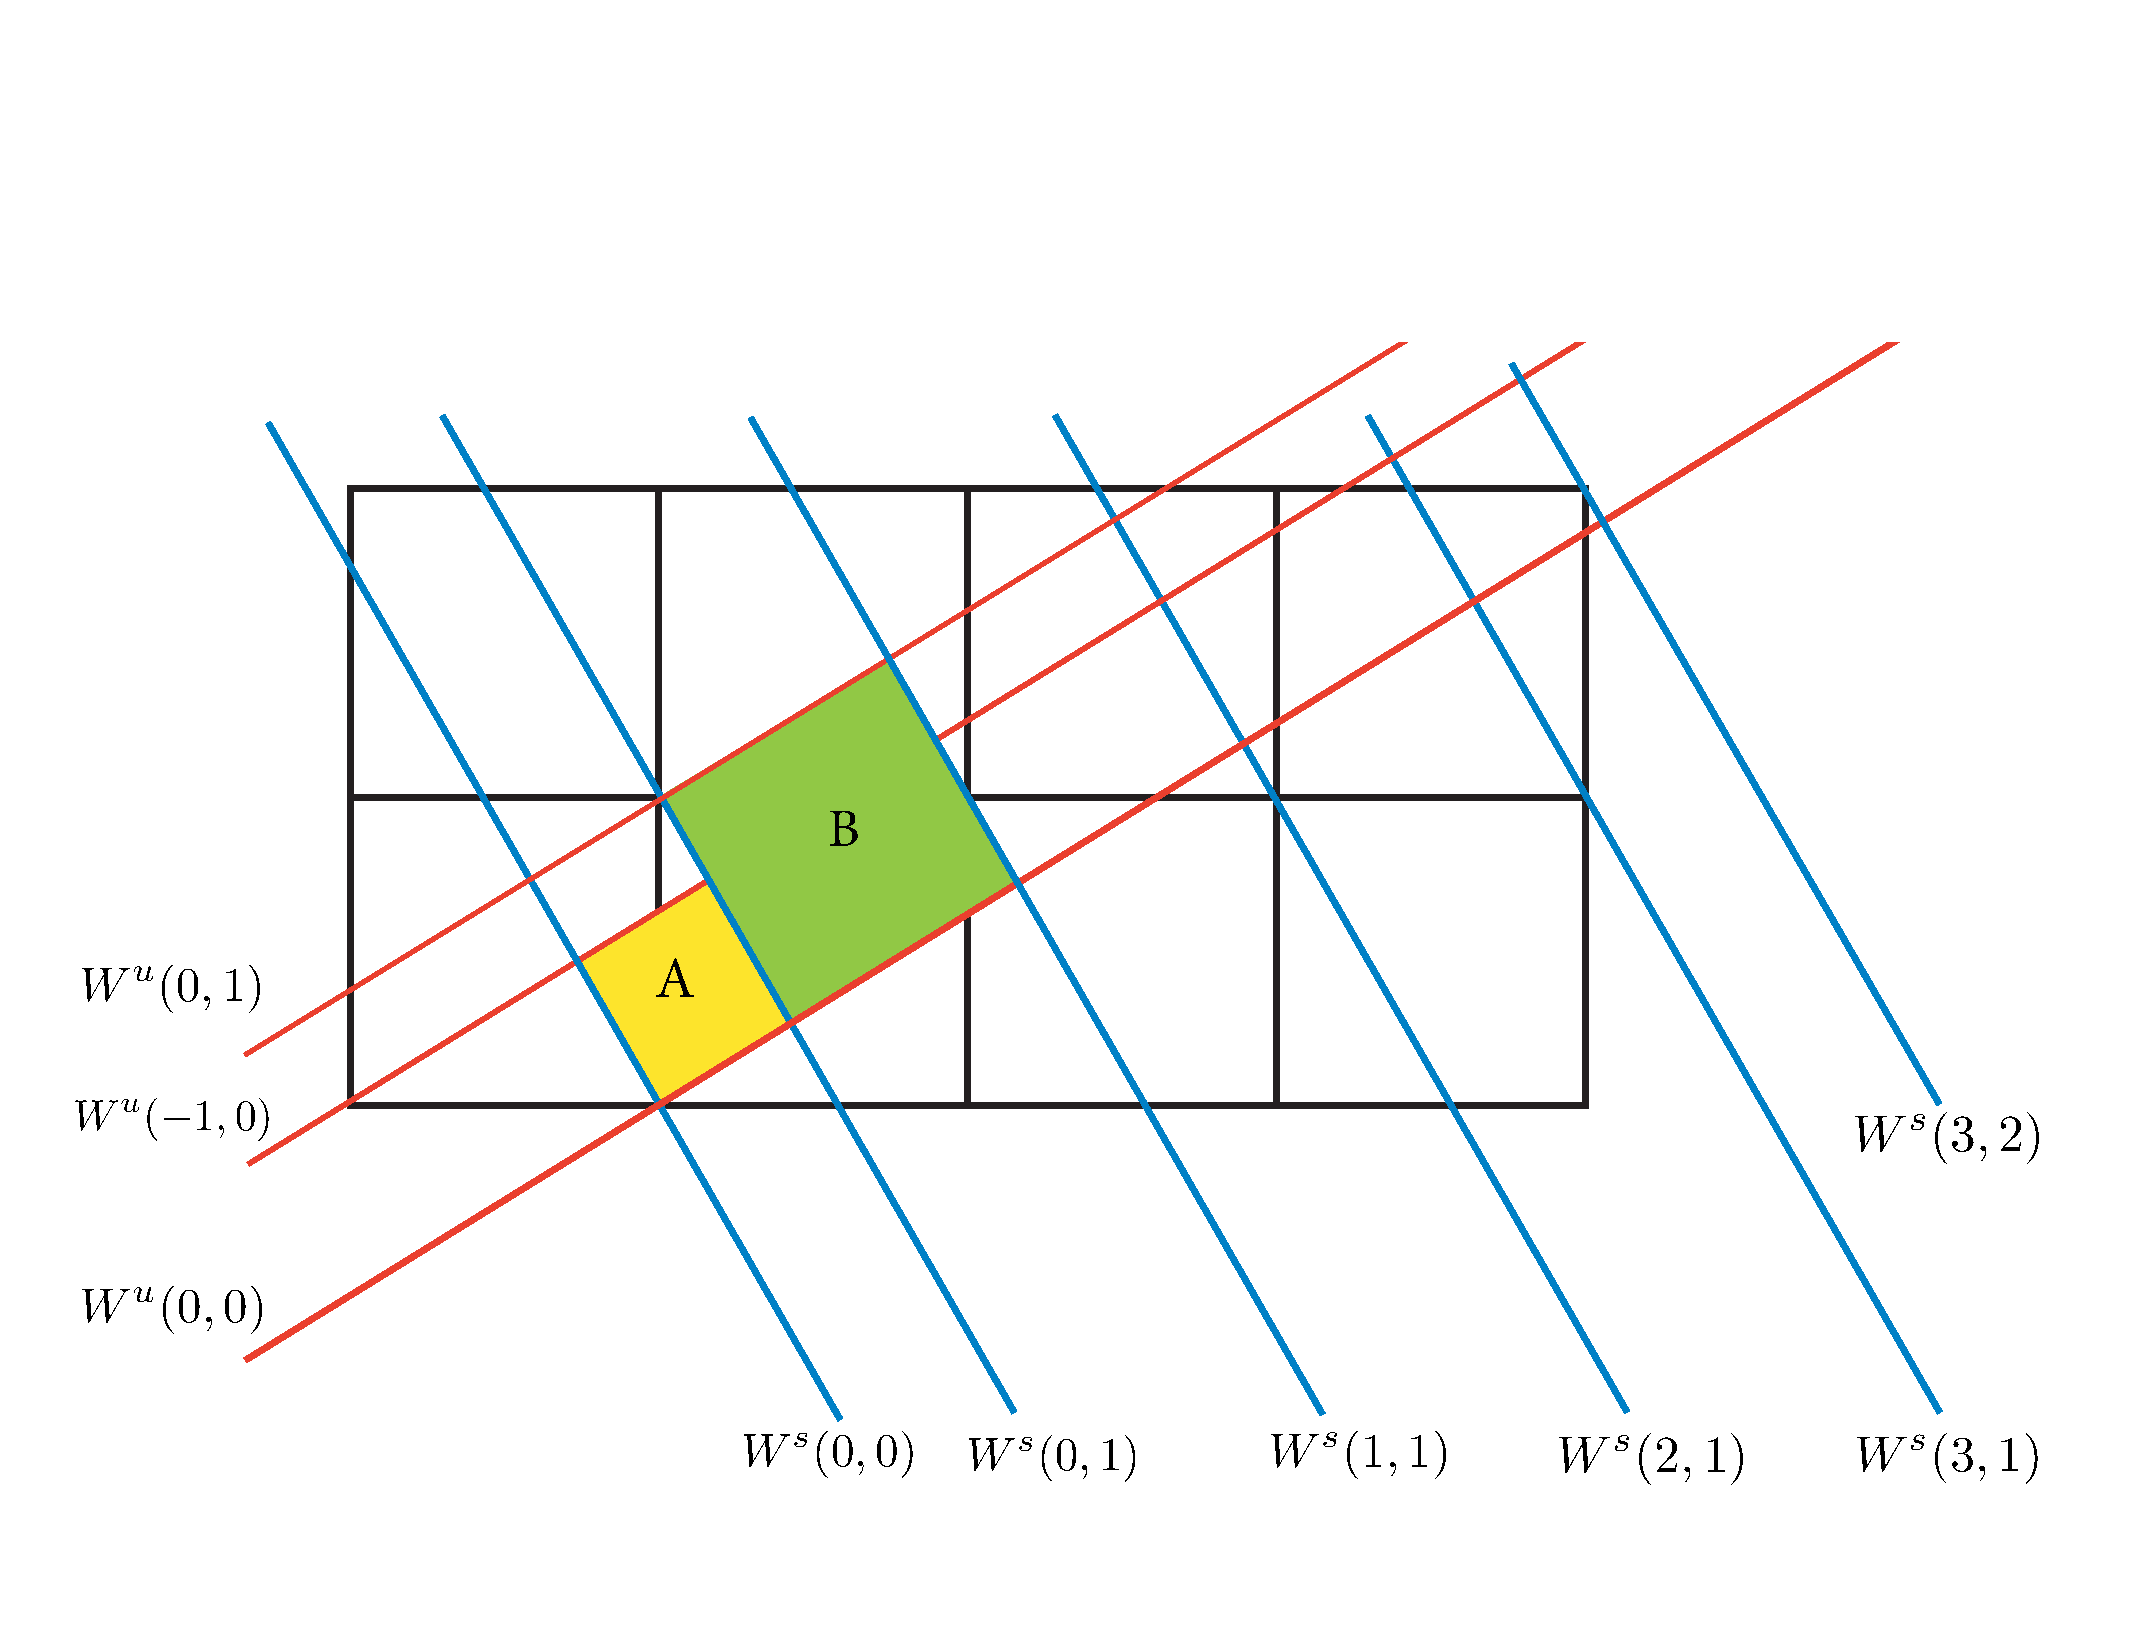
\includegraphics[width=0.74\textwidth]{Lect13p8}
\\
(b) 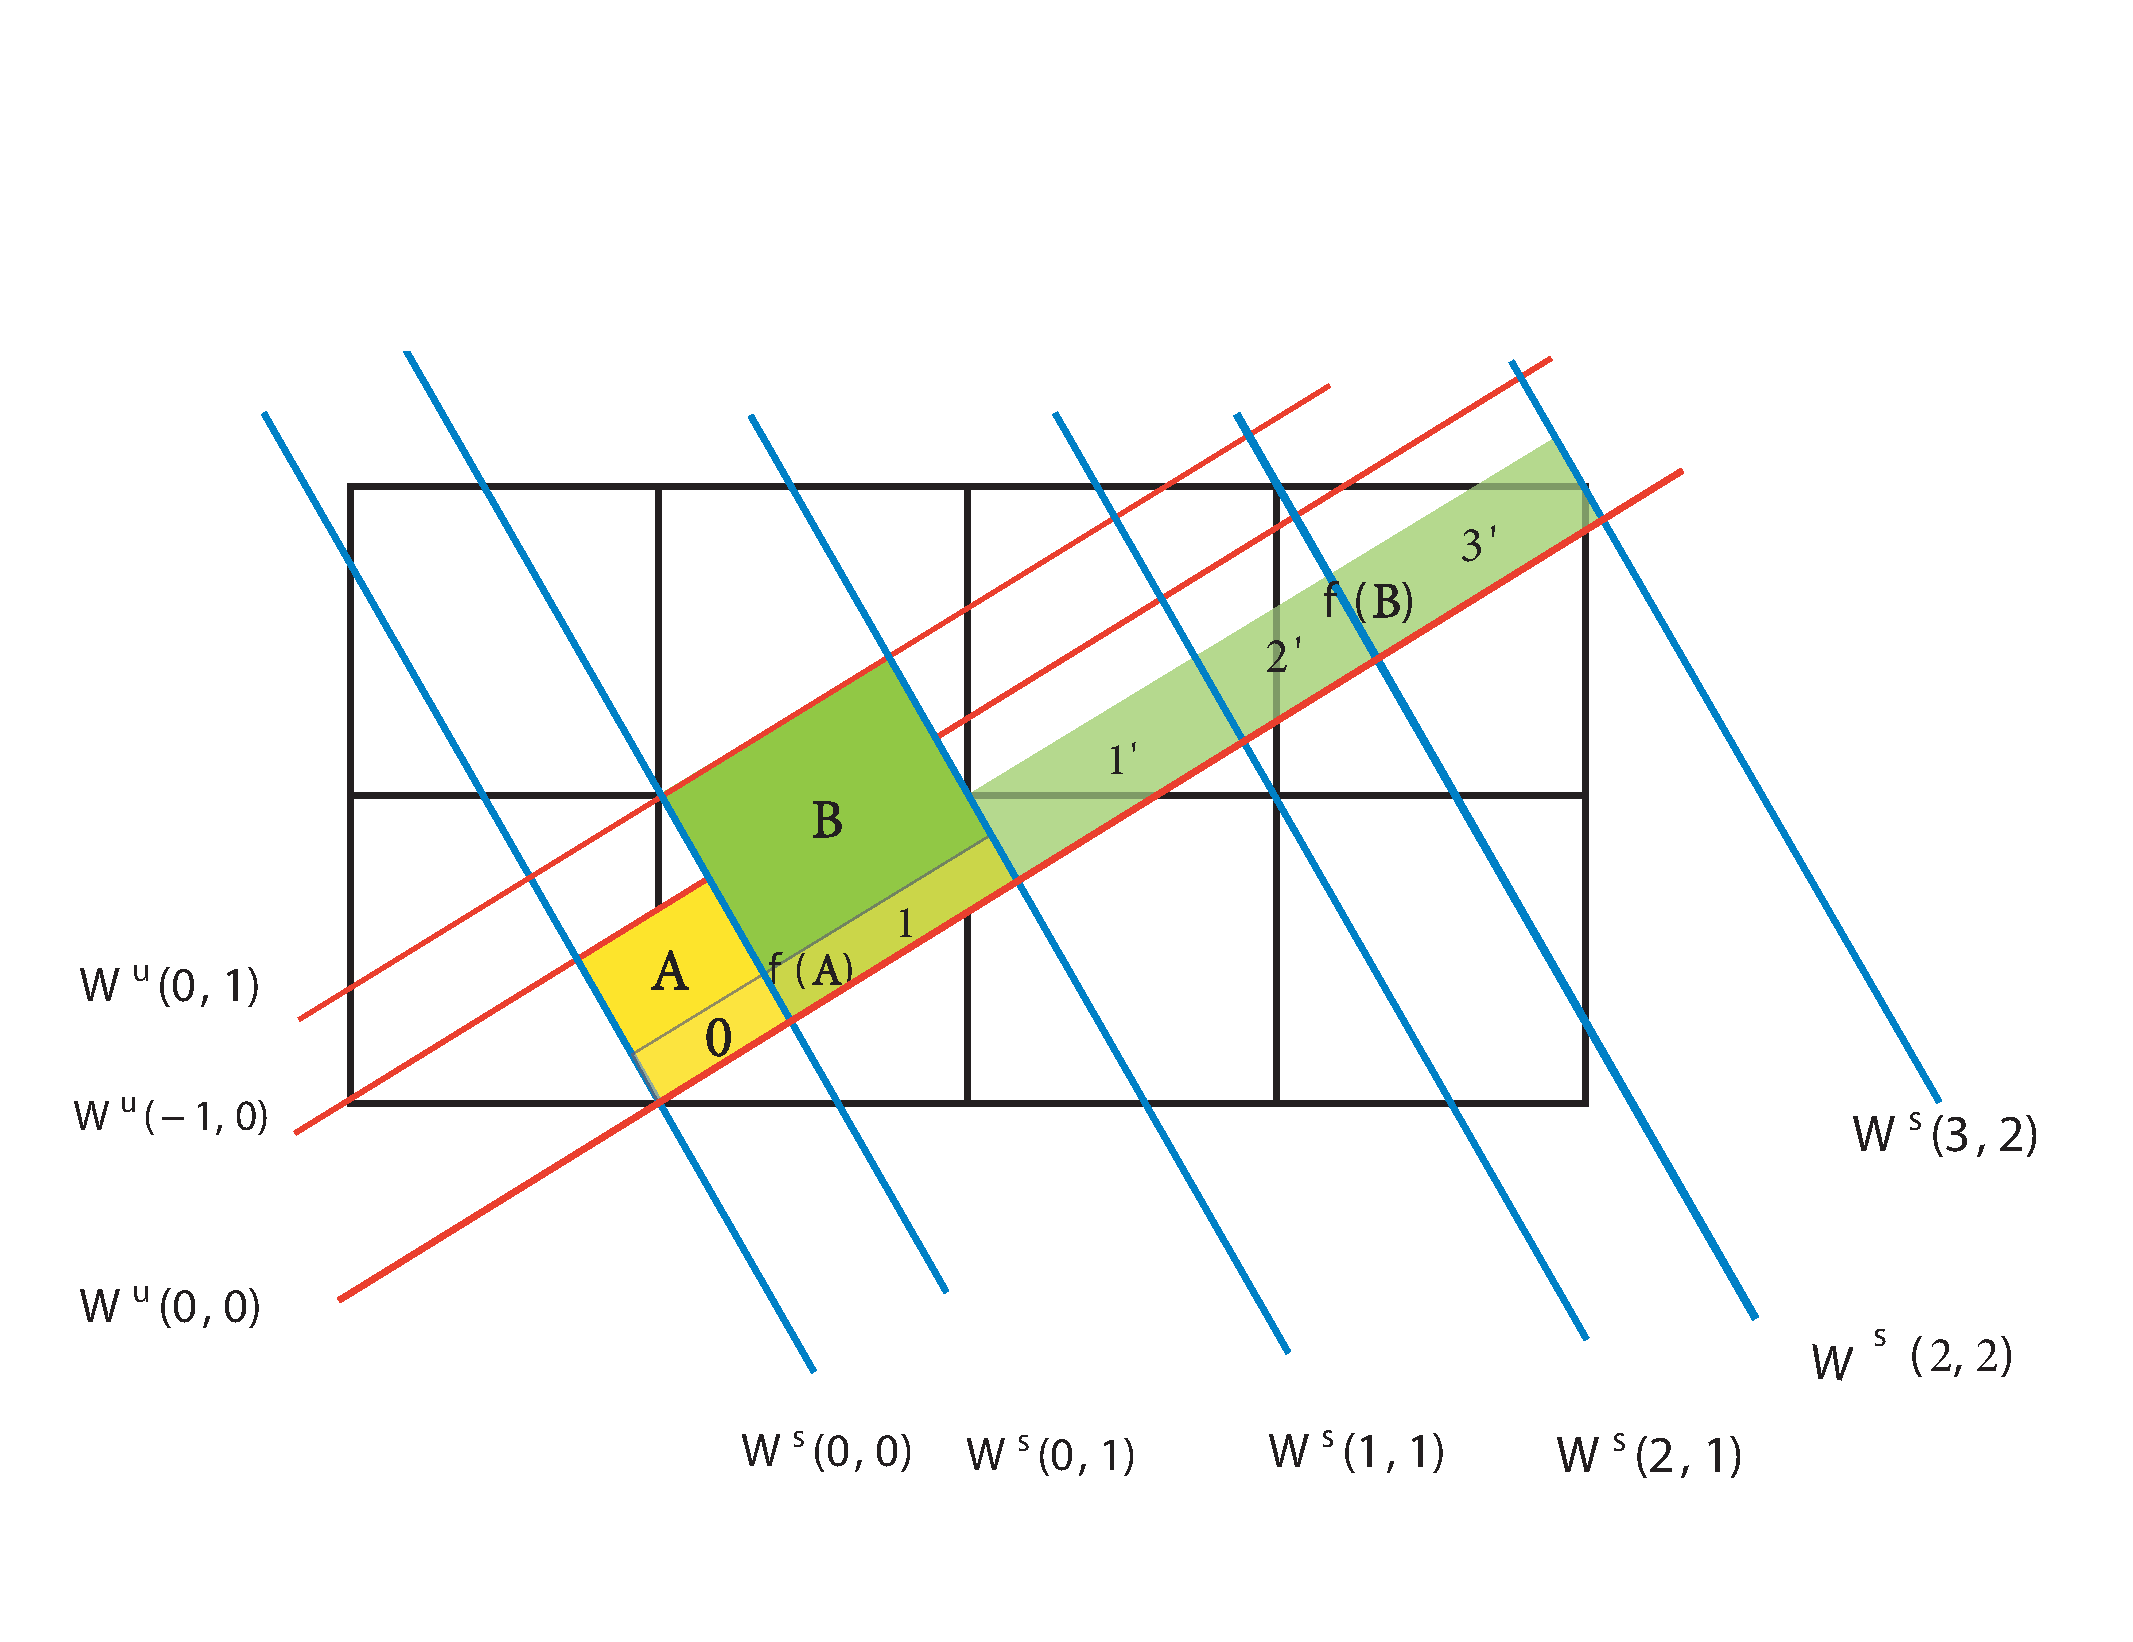
\includegraphics[width=0.74\textwidth]{Lect13p11}
\\
(c)  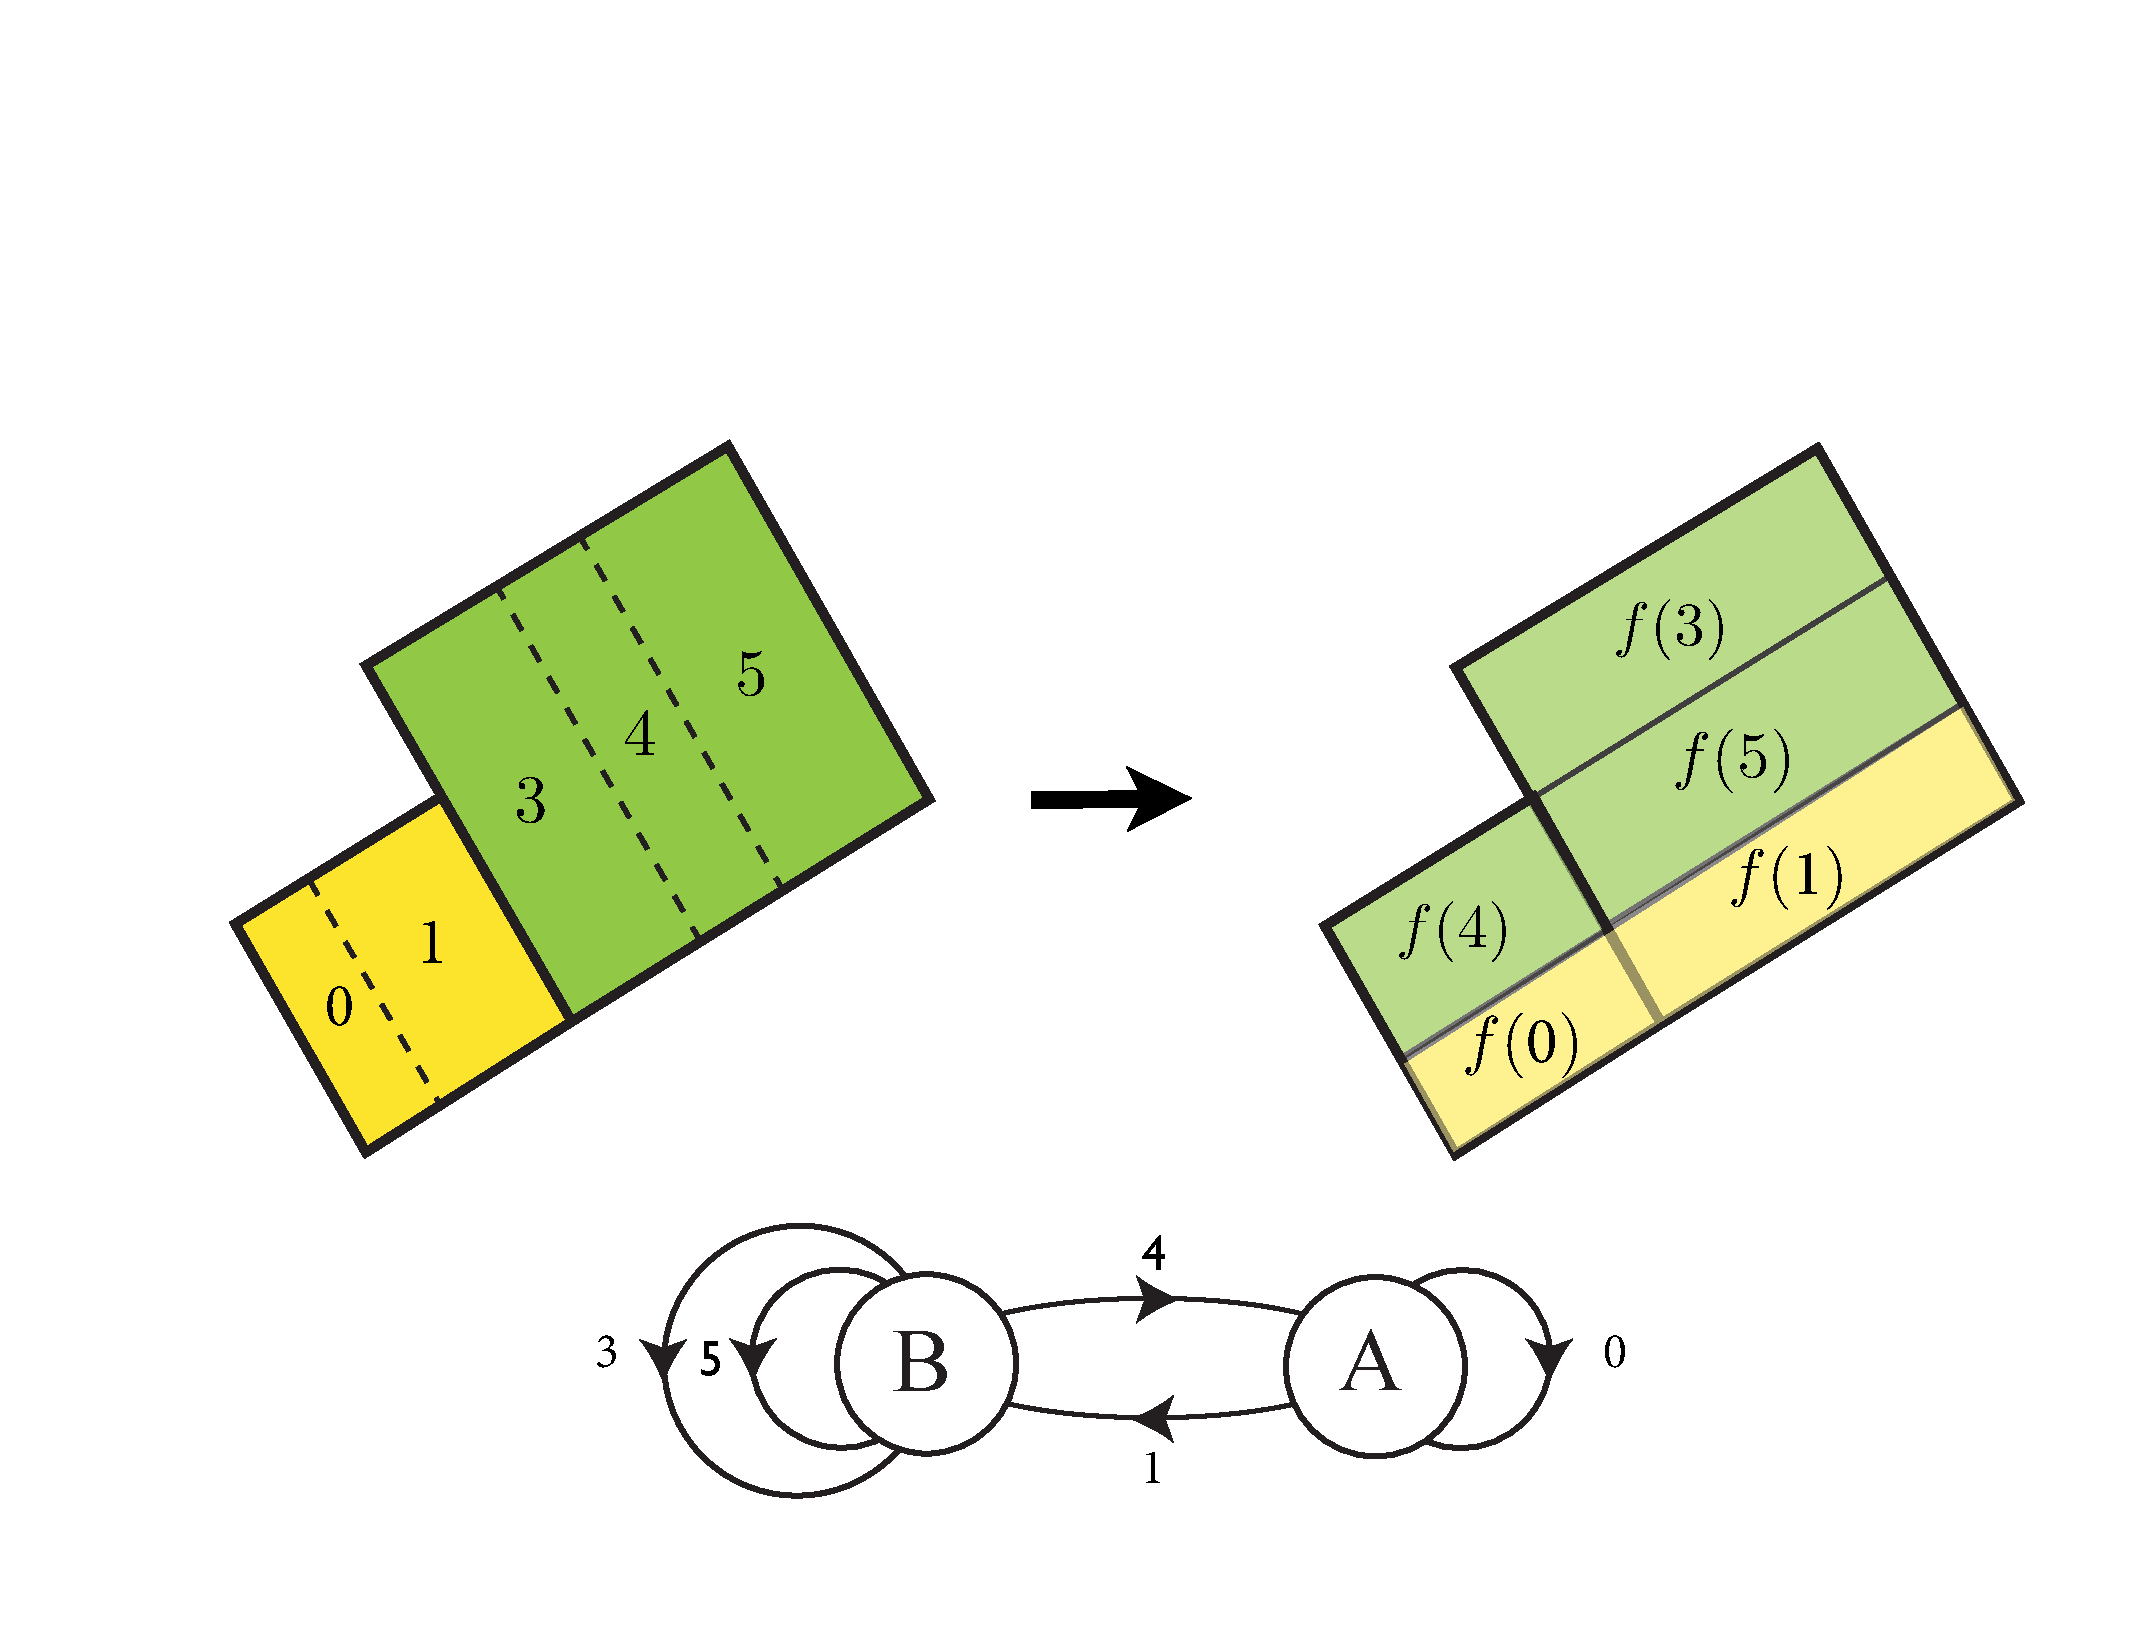
\includegraphics[width=0.5\textwidth]{Lect13p17}
  \caption{\label{fig:Lect13p8}
(a) Two-rectangles \AW\ generating partition for the canonical Arnol'd cat
map \refeq{ArnoldCat}, with borders given by stable-unstable manifolds of the
unfolded cat map lattice points near to the origin.
(b) The first iterate of the partition.
(c) The iterate pulled back into the generating partition,
and the corresponding 5-letter {\markGraph}. In (b) and (c)
I have not bothered to
relabel Crutchfield partition labels with our
shift code. This is a ``linear code,'' in the
sense that for each square on can count how many side-lengths are needed
to pull the overhanging part of $f(x)$ back into the two defining squares.
(Figure by Crutchfield\rf{Crutchfield18})
}
\end{figure}
%%%%%%%%%%%%%%%%%%%%%%%%%%%%%%%%%%%%%%%%%%%%%%%%%%%%%%%%%%%%%%


\refFig{fig:Lect13p8} for the canonical
Thom-Arnol'd cat map
                            \toRem{rem:catMapAbout}
\beq
A =
\MatrixII{2}{1}
         {1}{1}
\,.
% \qquad\det A= 1 \,,
\ee{ArnoldCat}

String people, \arXiv{1608.07845}, find the identity
\beq
\MatrixII{2}{1}
         {1}{1}
=
\MatrixII{1}{1}
         {0}{1}
\MatrixII{1}{0}
         {1}{1}
% = LR^{-1}
= L\transp{L}
%\,,
% \qquad\det A= 1 \,,
\ee{AxFlNi16(2.7)}
significant: ``The map corresponds to successive kicks, forwards and
backwards along the light cone [...]''

% 2018-02-10}{
As another example, with $s=4$,
Manning\rf{Manning02} discusses a Markov partition for the cat map
(also discussed by Anosov, Klimenko and Kolutsky\rf{AnKlKo08})
\beq
A =
\MatrixII{3}{1}
         {2}{1}
\,.
% \qquad\det A= 1 \,,
\ee{ArnoldCat2}

                                        \toCB
In order to count all admissible walks, one associates with the \markGraph\
such as the one in \reffig{fig:Lect13p8}\,(c) the {\em connectivity} matrix
\beq
C =
\MatrixII{1}{1}
         {1}{2}
\,,
\ee{connArnoldCat}
where $C_{ij}$ is the number of ways (number of links) of getting to $i$ from
$j$.



\section{\AW\ partition of the \PV\ cat map}
\label{sect:AdlWeiPV}

%\item[2016-05-29 PC]
%I have added this chapter with intention to include it as several examples
%in ChaosBook.org.

%%%%%%%%%%%%%%%%%%%%%%%%%%%%%%%%%%%%%%%%%%%%%%%%%%%%%%%%%%%%%%%%
  \begin{figure}
  \begin{center}  %%% 2016-12-25  see
                  %%% siminos/figsSrc/inkscape/CatMapStatesp.svg
  \setlength{\unitlength}{0.65\textwidth}
 %% \unitlength = units used in the Picture Environment
  \begin{picture}(1,0.81984366)%
    \put(0,0){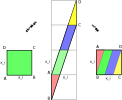
\includegraphics[width=\unitlength]{CatMapStatesp}}%
    \put(-0.025,0.15){\color[rgb]{0,0,0}\makebox(0,0)[lb]{\smash{$(0,0)$}}}%
    \put(0.26669086,0.17307744){\color[rgb]{0,0,0}\makebox(0,0)[lb]{\smash{B}}}%
    \put(0.26669086,0.41839762){\color[rgb]{0,0,0}\makebox(0,0)[lb]{\smash{C}}}%
    \put(0.02137069,0.41839762){\color[rgb]{0,0,0}\makebox(0,0)[lb]{\smash{D}}}%
    \put(0.38935094,0.00135332){\color[rgb]{0,0,0}\makebox(0,0)[lb]{\smash{B}}}%
    %\put(0.32,0.17){\color[rgb]{0,0,0}\makebox(0,0)[lb]{\smash{$(0,0)$}}}%
    \put(0.64284833,0.60647641){\color[rgb]{0,0,0}\makebox(0,0)[lb]{\smash{C}}}%
    \put(0.64284833,0.79455521){\color[rgb]{0,0,0}\makebox(0,0)[lb]{\smash{D}}}%
    %\put(0.79004043,0.42657495){\color[rgb]{0,0,0}\makebox(0,0)[lb]{\smash{A}}}%
    %\put(0.79004043,0.17307744){\color[rgb]{0,0,0}\makebox(0,0)[lb]{\smash{B}}}%
    %\put(0.96994189,0.17307744){\color[rgb]{0,0,0}\makebox(0,0)[lb]{\smash{C}}}%
    %\put(0.97811923,0.42657495){\color[rgb]{0,0,0}\makebox(0,0)[lb]{\smash{D}}}%
    \put(0.02,0.27){\color[rgb]{0,0,0}\rotatebox{90.0}{\makebox(0,0)[lb]{\smash{$\ssp_{0}$}}}}%
    \put(0.39,0.27){\color[rgb]{0,0,0}\rotatebox{90.0}{\makebox(0,0)[lb]{\smash{$\ssp_{1}$}}}}%
    \put(0.76,0.27){\color[rgb]{0,0,0}\rotatebox{90.0}{\makebox(0,0)[lb]{\smash{$\ssp_{1}$}}}}%
    \put(0.1469525,0.173){\color[rgb]{0,0,0}\makebox(0,0)[lb]{\smash{$\ssp_{-1}$}}}%
    \put(0.51493279,0.174){\color[rgb]{0,0,0}\makebox(0,0)[lb]{\smash{$\ssp_{0}$}}}%
    \put(0.86655824,0.175){\color[rgb]{0,0,0}\makebox(0,0)[lb]{\smash{$\ssp_{0}$}}}%
    \put(0.21762677,0.55482852){\color[rgb]{0,0,0}\rotatebox{43.35476392}{\makebox(0,0)[lb]{\smash{stretch}}}}%
    \put(0.74915379,0.61465381){\color[rgb]{0,0,0}\rotatebox{-46.94301089}{\makebox(0,0)[lb]{\smash{wrap}}}}%
  \end{picture}%
\end{center}
   \caption{ \label{fig:CatMapStatesp}
(Color online)
The $s=3$  \PV\ cat map matrix \refeq{PerViv:2confRepMat}
%\refeq{eq:StateSpCatMap} keeps the origin $(0,0)$ fixed, but otherwise
stretches the unit square
into a parallelogram. Translations by $\Ssym{0}$ from alphabet
$\A=\{-1,0,1,2\}=$
\{%
{\color{red}red},
{\color{green}green},
{\color{blue}blue},
{\color{yellow}yellow}%
\}
bring stray regions back onto the torus.
   }
 \end{figure}
%%%%%%%%%%%%%%%%%%%%%%%%%%%%%%%%%%%%%%%%%%%%%%%%%%%%%%%%%%%%%%%%

%    \PCpost{2016-12-26}{
As illustrated in \reffig{fig:CatMapStatesp}, the action of the
cat map in the \PV\rf{PerViv}  ``two-configuration
representation'' is given by the antisymmetric  area
preserving $[2\!\times\!2]$ matrix
\beq
{\bf A}
=\MatrixII{0}{1}
          {-1}{s}
\ee{PerViv:2confRepMat}
For the Arnol'd value $s=3$,
in one time step the map stretches the unit square into a parallelogram, and
than wraps it around the torus 3 times, as in \reffig{fig:CatMapStatesp}.
Visualise the phase space as a bagel, with $\ssp_0$ axis a circle on the
outside of the bagel. This circle is divided into three color segments, which
map onto each other as you got in the $\ssp_1$ axis direction.  Now apply the
inverse map - you get 3 strips intersecting the the above strips, for 9
rectangles in all: a full shift, \ie, a ternary Smale horseshoe. So on the
torus there are only 3 strips - there is no distinction between the two outer
letters $\Ae=\{-1,2\}=$
\{%
{\color{red}red},
{\color{yellow}yellow}%
\},
it is the same third strip. The division into 2 triangles is an artifact
of plotting the torus as a unit square. All
complicated pruning of (the current draft of) Gutkin \etal\rf{GHJSC16}
is a red herring, due to over-partitioning of the
torus with a 4-letter alphabet.

{\em This is stupid.}

How do \AW\ coordinates work out for the Arnol'd cat map in the \PV\
representation \refeq{PerViv:2confRepMat} used here?
First one needs to construct the eigen-coordinates.

%%%%%%%%%%%%%%%%%%%%%%%%%%%%%%%%%%%%%%%%%%%%%%%%%%%
\hfill         \fastTrackExam{exam:ProjOpCatMap}

For $s>2$ the stability multipliers
\(
(\ExpaEig^{+},\ExpaEig^{-})
\,=\,(\ExpaEig\,,\; \ExpaEig^{-1})
\)
are real,
\beq
\ExpaEig^{\pm}=\frac{1}{2}(s\pm \surd{D})
\,,\qquad
\ExpaEig=e^{\Lyap}
\,,
\ee{catEigs}
where
\bea
s&=&\ExpaEig+\ExpaEig^{-1}
  =  2\cosh(\Lyap)
    \,,\quad
    \continue
\surd{D}&=&\ExpaEig-\ExpaEig^{-1}
  =  2\sinh(\Lyap)
\label{catEigs1}
\eea
 discriminant $D=s^{2}-4$,
with a positive Lyapunov exponent $\Lyap >0$,
and the right, left eigen\-vectors:
\bea
\{ \jEigvec[+],\jEigvec[-] \} &=& \left\{
    \VectorII{\ExpaEig^{-1}}{1}
    \,,
     \VectorII{\ExpaEig}{1} \right\}
    \continue
\{ \jEigvecT[+],\jEigvecT[-] \} &=& \left\{
   [-\ExpaEig^{-1},1]
    \,,
    [\ExpaEig,-1] \right\}
\,,
\label{eigVecs}
\eea
(where the overall scale is arbitrary).
As the matrix is not symmetric, the
$\{\jEigvec[j]\}$ do not form an orthogonal basis.

What does this do to the partition of \reffig{fig:CatMapStatesp}? The origin
is still the fixed point. For a \statesp\ point in the new, dynamically
intrinsic right eigenvector \AW\ %\rf{AdWei70}
coordinate basis $x'$
\[
\left(\begin{array}{c}
 \ssp_{t-1}'  \\
 \ssp_{t}'
 \end{array} \right )
 =
\left(\begin{array}{c}
 -\ExpaEig\ssp_{t}+\ssp_{t-1}\\
 -\ExpaEig^{-1}\ssp_{t}+\ssp_{t-1}
 \end{array} \right )
\,.
\]
the abscissa ($\ssp_{t-1}$ direction) is not affected, but the ordinate
($\ssp_{t}$ direction) is flipped and stretched/shrunk by factor $-\ExpaEig$,
$-\ExpaEig^{-1}$ respectively,
\[
\left(\begin{array}{c}
 \ssp_{t}'  \\
 \ssp_{t+1}'
 \end{array} \right )
 =
 \MatrixII{\ExpaEig^{-1}}{0}
          {0}            {\ExpaEig}
\left(\begin{array}{c}
 \ssp_{t-1}'  \\
 \ssp_{t}'
 \end{array} \right )
 - \left(\begin{array}{c}
 0  \\
 \Ssym{t}
 \end{array} \right )
\,,
\]
preserving the vertical strip nature of the
partition of \reffig{fig:CatMapStatesp}. In the \AW\ right eigenbasis,
${\bf A}$ acts by stretching the $\jEigvec[+]$ direction by $\ExpaEig$, and
shrinking the $\jEigvec[-]$ direction by  $\ExpaEig^{-1}$, without any rotation
of either direction.

Thus the \AW\ coordinates preserve the convenient feature of the
\PV\ cat map, \reffig{fig:CatMapStatesp}: the torus `rewrapping'
translations remain all vertical, specified by a single integer.

The angles of stable / unstable manifolds are irrational respective to the
lattice, and they never hit another vertex (and so they do not close onto
themselves under quotienting of translations).

%%%%%%%%%%%%%%%%% by hand calculations :)
%   \surd{D} = sqrt(5)         = 2.23606797749
%   L1 = (3+sqrt(5))/2  = 2.61803398874
%   L2 = (3-sqrt(5))/2  = 0.38196601125
%   e11= (L2)/(\surd{D})       = 0.17082039325
%   e12= (1)/(\surd{D})        = 0.44721359550
%   e21= (L1)/(\surd{D})       = 1.17082039325
%   e22= (1)/(\surd{D})        = 0.44721359550
%
%   y = e12/e11         = 2.61803398874 x slope expanding
%   y = e21/e22         = 0.38196601125 x slope contracting
%
% contract: Plot[0.38196601125 x, {x, 0, 1}, {y, 0, 1}]
% expand:   Plot[2.61803398874 x, {x, 0, 1}, {y, 0, 1}] width 10.509
%
% horizontally along x:
%  (439.8005-343.6351)*0.381966+343.6351 = 380.367, got through x= 232.17
%  (-143.732+195.435)*0.381966 = 36.734, got through x= 175.7
% vertically along y:
%  (496.6877-400.3766)*2.6180+400.3766   = 652.519, got through x= 195.0420
%  (155.5237-103.7766)*2.6180+103.7766   = 239.25, got through x= 195.0420


%%%%%%%%%%%%%%%%%%%%%%%%%%%%%%%%%%%%%%%%%%%%%%%%%%%%%%%%%%%%%%%%%
%  \begin{figure}
%  \begin{center}  %%% 2016-12-25  see
%[to be drawn]
%\end{center}
%   \caption{ \label{fig:CatMapEigVecs}
%(Color online)
%Going from the Newtonian $s=3$  Arnol'd cat map to the right eigenvector
%\AW\ coordinate basis,
%with the expanding (purple) and contracting (beige) eigendirections indicated.
%Next: figure out the two rectangles which are the start of the \AW\
%construction. Or three rectangles - would be nice to have a partition something
%symmetric across the main diagonal, as the two eigendirections are symmetric
%under time reversal.
%   }
% \end{figure}
%%%%%%%%%%%%%%%%%%%%%%%%%%%%%%%%%%%%%%%%%%%%%%%%%%%%%%%%%%%%%%%%%

%%%%%%%%%%%%%%%%%%%%%%%%%%%%%%%%%%%%%%%%%%%%%%%%%%%%%%%%%%%%%
\begin{figure}
  \centering
(a)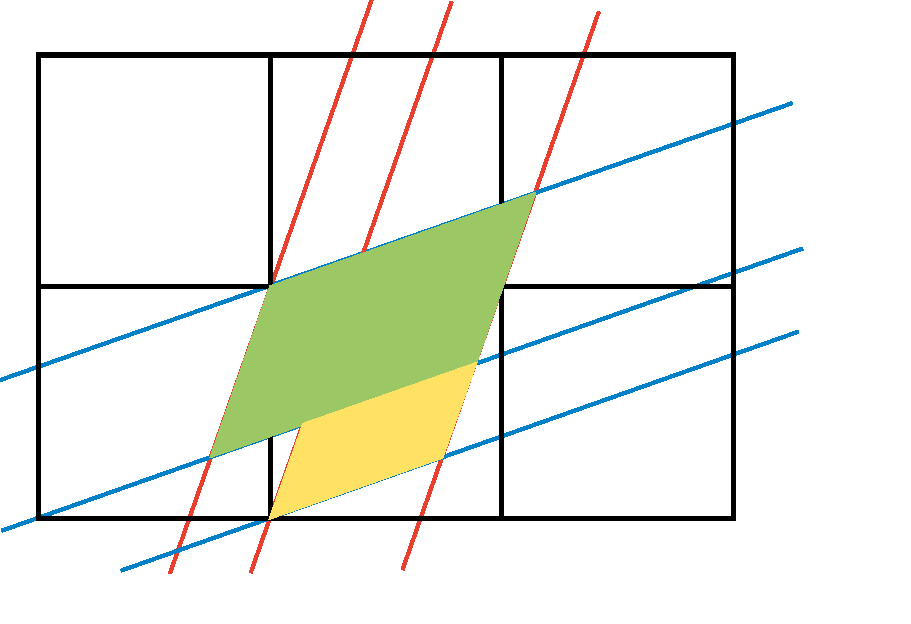
\includegraphics[width=0.40\textwidth]{PCLect13p8}
(b)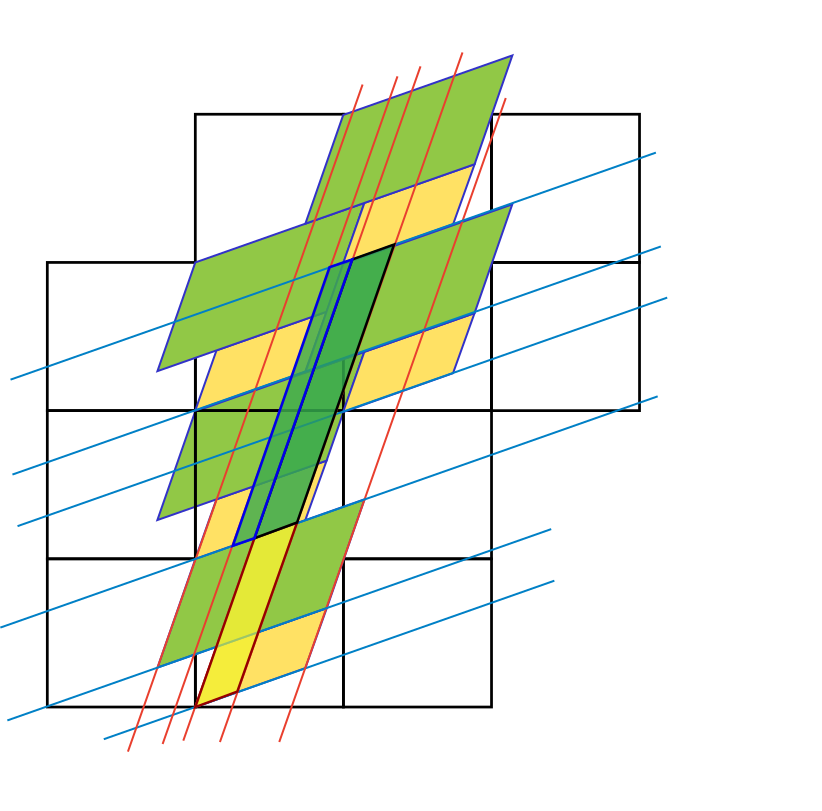
\includegraphics[width=0.50\textwidth]{PCLect13p14}
  \caption{\label{fig:PCLect13p8}
(a) An abandoned two-rectangle \AW\ generating
partition for the \PV\ cat map \refeq{PerViv:2confRepMat}, with
borders given by cat map stable-unstable manifolds.
(b) An abandoned attempt to identify the finite partition,
since superseded by the partition of \reffig{fig:PCLect13p16}\,(b)
and \reffig{fig:PVAdlerWeissB}.
}
\end{figure}
%%%%%%%%%%%%%%%%%%%%%%%%%%%%%%%%%%%%%%%%%%%%%%%%%%%%%%%%%%%%%%%

%%%%%%%%%%%%%%%%%%%%%%%%%%%%%%%%%%%%%%%%%%%%%%%%%%%%%%%%%%%%%
\begin{figure}
  \centering
(a)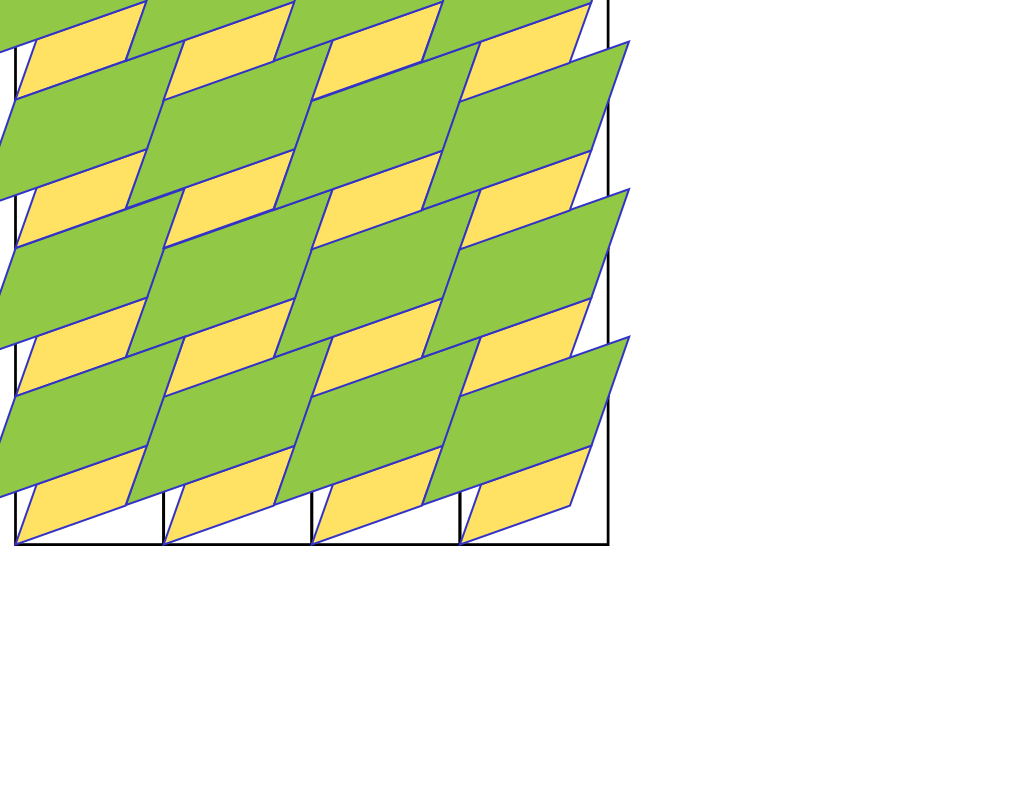
\includegraphics[width=0.45\textwidth]{PCLect13p12}
(b)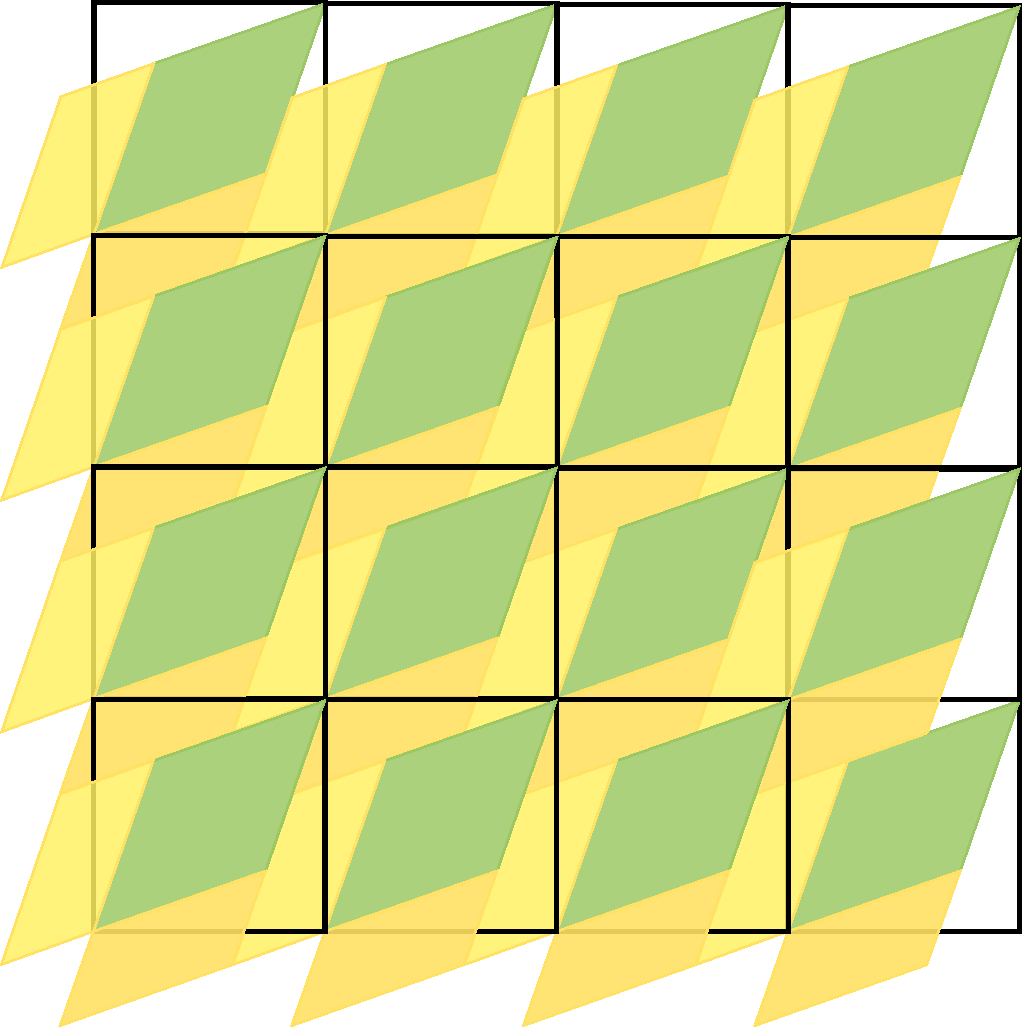
\includegraphics[width=0.45\textwidth]{PCLect13p13}
  \caption{\label{fig:PCLect13p12}
(a) [Abandoned] Tiling of the square lattice by the two-rectangle \AW\
generating partition of \reffig{fig:PCLect13p8}\,(a) for the \PV\
cat map \refeq{PerViv:2confRepMat}.
(b) Tiling of the square lattice by the three-rectangle, time reversal
symmetric generating partition. Note that we have used the continuous
translation invariance to center the large tile $A$ within the
unit square (continued in \reffig{fig:PCLect13p9}\,(a)).
}
\end{figure}
%%%%%%%%%%%%%%%%%%%%%%%%%%%%%%%%%%%%%%%%%%%%%%%%%%%%%%%%%%%%%%%

Note that from \reffig{fig:PCLect13p12}\,(a) to
\reffig{fig:PCLect13p12}\,(b) we have used the continuous translation
invariance to center the large tile $A$ within the unit square. That
makes the time reversal invariance more explicit.
It might not be obvious that the two parallelograms of
\reffig{fig:PCLect13p8}\,(a) tile the square lattice, but they do, as
illustrated in \reffig{fig:PCLect13p12}\,(a).
                                            \toRem{rem:PythagorTiling}
Such tilings are known as `Pythagorean'.

Given the stable/unstable eigenvectors, the
natural eigen-coordinates are given. I had first constructed a
2-rectangle generating partition for the \PV\rf{PerViv}
two-configuration representation \refeq{PerViv:2confRepMat} - it is a squashed
and rotated version of \reffig{fig:Lect13p8}\,(a)
drawn in \reffig{fig:PCLect13p8}\,(a). The point is, after a
linear change of coordinates one has finite grammar \AW\ symbolic
dynamics, and the symbolic dynamics is a linear code in sense of Boris,
but this time with all admissible sequences generated as walks on
a \markGraph\ isomorphic to the one in \reffig{fig:Lect13p8}\,(c).

I actually like better the three-rectangle, time reversal symmetric
generating partition of \reffig{fig:PCLect13p9} and \reffig{fig:PCLect13p16}.

%%%%%%%%%%%%%%%%%%%%%%%%%%%%%%%%%%%%%%%%%%%%%%%%%%%%%%%%%%%%%
\begin{figure}
  \centering
(a)~~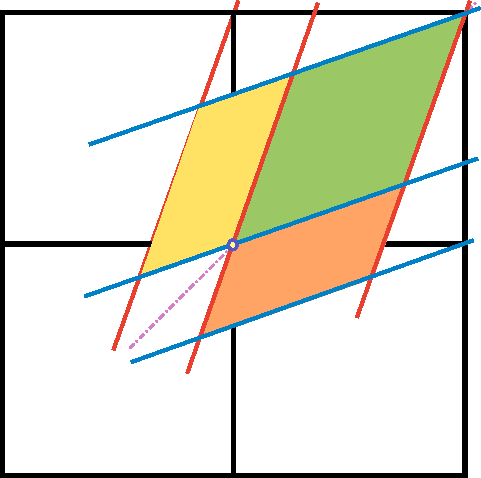
\includegraphics[width=0.37\textwidth]{PCLect13p9}
(b)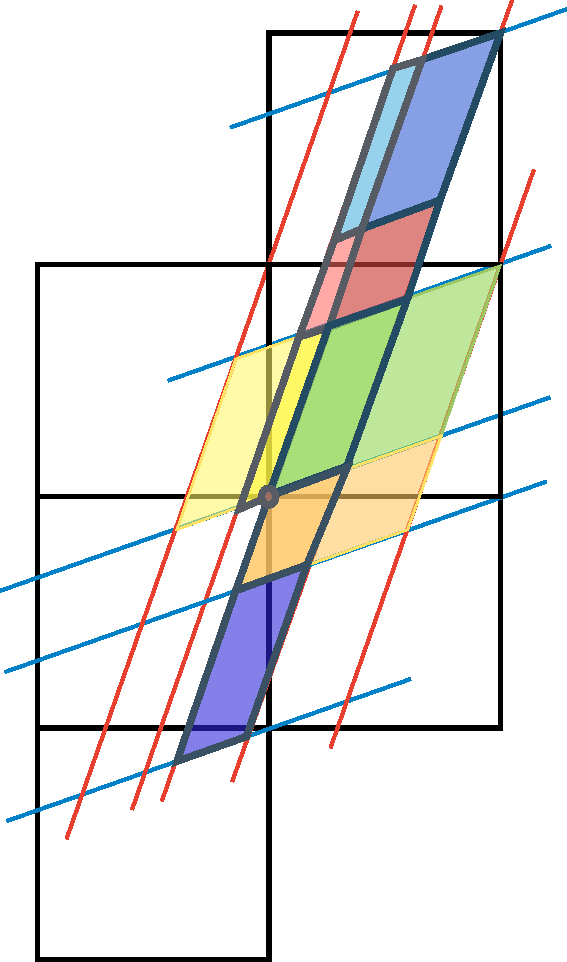
\includegraphics[width=0.41\textwidth]{PCLect13p15}
  \caption{\label{fig:PCLect13p9}
(a) The three-rectangle, time reversal symmetric generating partition
for the \PV\ cat map \refeq{PerViv:2confRepMat}, with borders given by cat
map stable-unstable manifolds.
(b) The three-rectangle mapped one step forward in time.
}
\end{figure}
%%%%%%%%%%%%%%%%%%%%%%%%%%%%%%%%%%%%%%%%%%%%%%%%%%%%%%%%%%%%%%%

%%%%%%%%%%%%%%%%%%%%%%%%%%%%%%%%%%%%%%%%%%%%%%%%%%%%%%%%%%%%%
\begin{figure}
  \centering
(a)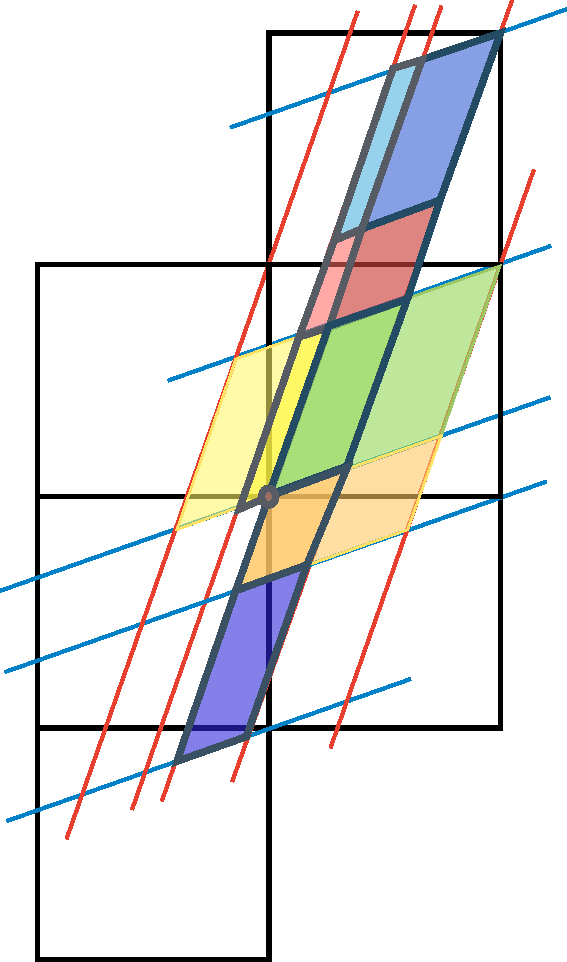
\includegraphics[width=0.30\textwidth]{PCLect13p15}
(b)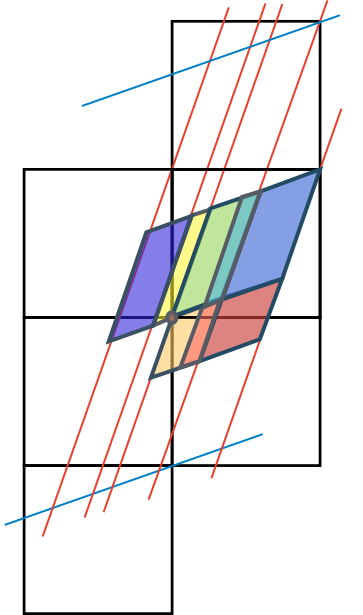
\includegraphics[width=0.30\textwidth]{PCLect13p16}
  \caption{\label{fig:PCLect13p16}
(a) The three-rectangle mapped one step forward in time.
(b) The three-rectangle wrapped back onto the torus, along the unstable
direction, yields 8-letter alphabet generating partition, with three-nodes
\markGraph.
One could have kept the two-rectangle \AW\ generating partition of
\reffig{fig:PCLect13p8}\,(a), in which case the alphabet is the standard 5
letters.
}
\end{figure}
%%%%%%%%%%%%%%%%%%%%%%%%%%%%%%%%%%%%%%%%%%%%%%%%%%%%%%%%%%%%%%%

%%%%%%%%%%%%%%%%%%%%%%%%%%%%%%%%%%%%%%%%%%%%%%%%%%%%%%%%%%%%%
\begin{figure}
  \centering
(a)~~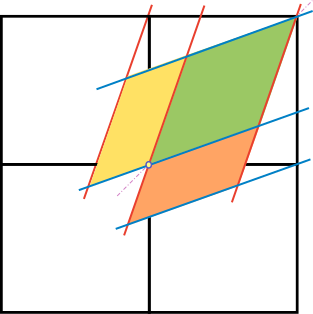
\includegraphics[width=0.37\textwidth]{PCLect13p9b}
(b)~~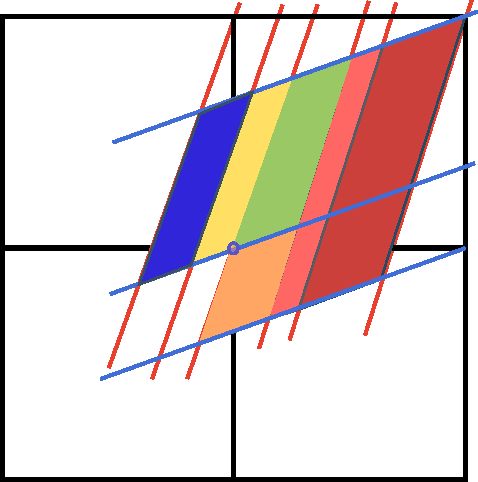
\includegraphics[width=0.37\textwidth]{PCLect13p16a}
  \caption{\label{fig:PPCLect13p16a}
\refFig{fig:PCLect13p16} continued.
(a) The three-rectangle, time reversal symmetric generating partition for
the \PV\ cat map \refeq{PerViv:2confRepMat}, with borders given
by cat map stable-unstable manifolds.
(b) The three-rectangle subpartition, one step forward in time. $A$ into three
strips, $B$ into three strips, $B'$ into two strips, for a total of 8
forward links in the graph
 \PCedit{continue with a sensible coloring of these regions)}.
Label the graph links by
translations that bring these pieces back into the unit square.
Under time reversal, interchange $B$ and $B'$, get the same partition going
backwards in time. Then make it Lagrangian, meaning the combined graph should
have undirected links (?).
}
\end{figure}
%%%%%%%%%%%%%%%%%%%%%%%%%%%%%%%%%%%%%%%%%%%%%%%%%%%%%%%%%%%%%%%


%%%%%%%%%%%%%%%%%%%%%%%%%%%%%%%%%%%%%%%%%%%%%%%%%%%%%%%%%%%%%
\begin{figure}
  \centering
(a)~~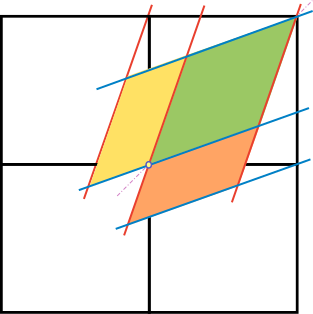
\includegraphics[width=0.37\textwidth]{PCLect13p9b}
(b)~~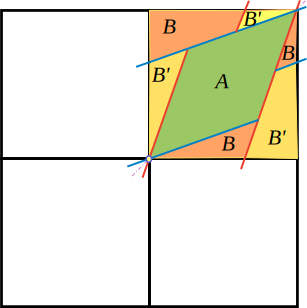
\includegraphics[width=0.37\textwidth]{PCLect13p9c}
  \caption{\label{fig:PCLect13p9b}
(a) The three-rectangle, time reversal symmetric generating partition for
the \PV\ cat map \refeq{PerViv:2confRepMat}, with borders given
by cat map stable-unstable manifolds.
(b) The three-rectangle partition of the unit square (torus laid out).
In this partition $A$ already lies entirely within the unit square,
while
$B$ and
$B'$ are wrapped around the torus, and only seem to consist of three pieces
each,
an artifact of the wrapping. The unit square borders have no physical meaning.
}
\end{figure}
%%%%%%%%%%%%%%%%%%%%%%%%%%%%%%%%%%%%%%%%%%%%%%%%%%%%%%%%%%%%%%%

Thus we have constructed \PV\ cat map coordinate transformation
from the square to the intrinsic \AW\ eigencoordinate basis. This is a
LINEAR transformation. As this has been falling on deaf ears for last few years,
let me say it again:

\bigskip\bigskip

This is a {\Huge LINEAR code},

\bigskip\bigskip

\noindent
as is every code in
Chaos\-Book, as illustrated by the examples of \refsect{exam:tentMapSymbDyn} that
I worked out for feline pleasure some years back. Got that?

As \AW\ partition is generating, there is noting for Dirichlet boundary
conditions Green's functions to accomplish - all admissible symbol {\brick s} are
known. The problem is now \emph{trivial}, in the Soviet sense (\ie, after a few years of
work, I understand it).

\bigskip

What is wrong with the argument so far? I used Newtonian, evolution-in-time
thinking to generate the $d=1$ partition. That will not work in higher
dimensions, so the above argument has to be recast in the Lagrangian form.

\bigskip

%Next: show that for $s=3$ the linear code in the new basis labels a
Be my guest - I'm going to bed:)

\bigskip

A few side, symmetry related remarks: we \emph{must} quotient translation
symmetries, do calculations in the elementary cell or, better still, the
fundamental domain.

\newpage
% siminos/kittens/catHamilton.tex                   pdflatex CL18
% $Author: predrag $ $Date: 2020-12-19 00:52:16 -0500 (Sat, 19 Dec 2020) $

\section{\AW\ partition of the cat map \statesp}
\label{s:catMapHam}

    \PC{2020-12-17}{
Remove from here, relink, once incorporated in ChaosBook.
    }
As explained in the companion paper\rf{GHJSC16},
the deep problem with the \PV\ code prescription is that it does not
yield a generating partition; the borders (\ie, $\ssp_0$, $\ssp_1$ axes)
of their unit-square partition
$(\ssp_{\zeit-1},\ssp_{\zeit})\in(0,1]\times(0,1]$
do not map onto themselves, resulting in the infinity of, to us unknown,
grammar rules for {\inadmissible} symbol sequences.

This problem was resolved in 1967 by Adler and
Weiss\rf{AdWei67,ArnAve,AdWei70} who utilized the stable/\-unstable
manifolds of the fixed point at the origin to cover a unit area torus by
a two-rectangles generating partition; for the \PV\ cat map
\refeq{eq:StateSpCatMap}, such partition\rf{DasBuch} is drawn in
 reffig{fig:PVAdlerWeiss}. Following Bowen\rf{Bowen70}, one refers to
such parallelograms as `rectangles'; for details
see Devaney\rf{deva87}, Robinson\rf{Robinson12}, or
ChaosBook\rf{DasBuch}. Siemaszko and Wojtkowski\rf{SieWoj11} refer to
such partitions as the `Berg partitions', and Creagh\rf{Creagh94} studies
their generalization to weakly nonlinear mappings.

While Percival and Vivaldi were well aware of \AW\ partitions, they felt
that their ``coding is less efficient in requiring more symbols, but it
has the advantage of linearity.'' Our construction demonstrates that one
can have both:  an \AW\ generating cat map partition, and a linear code.
The only difference from the \PV\ formulation\rf{PerViv} is that one
trades the single unit-square cover of the torus of
\refeq{eq:StateSpCatMap} for the dynamically intrinsic, two-rectangles
cover, but the effect is magic - now every
infinite walk on the {\markGraph}
corresponds to a unique {\admissible} orbit $\{\ssp_{\zeit}\}$, and the
{\markGraph} generates all {\admissible} itineraries $\{\Ssym{\zeit}\}$.

To summarize:
an explicit \AW\ generating partition completely solves the Hamiltonian cat map
problem, in the sense that it generates all {\admissible} orbits.
Rational and irrational initial states generate periodic and ergodic
orbits, respectively\rf{PerViv87b,Keating91}, with every \statesp\ orbit
uniquely labeled by an {\admissible} bi-infinite itinerary of symbols
from alphabet \A.

    \PC{2020-02-08}{
Note:
$N_2=\Det\jMorb=({s}-2)({s}+2)$,
$N_3 %   = {s}^3-3{s}-2
    = ({s}-2)({s}+1)^2$,
$N_4 = ({s}-2)({s}+1)\,{s}^2$,
$N_5 = ({s}-2)(s^2+ s-1 )^2$.
I think the factorization is true for all $\cl{}$, as the $s=2$ Laplacian
has a zero mode (constant $\ssp_i$, I think).

an sequence of non-negative integers counting the orbits of
a map; the sequence of periodic points for that map.
    }

This derivation was based on the \AW\ generating partition, a clever
explicit visualization of the cat map dynamics, whose generalization to
several coupled maps (let alone spatially infinite coupled cat
maps lattice) is far from obvious: one would have to construct covers of
high-dimensional {\fundPip}s by sets of sub-volumes.
However, as Keating\rf{Keating91} explains, no such explicit generating
partition is needed to count cat map \po s.

    % PC: restore here, once GHJSC16 finalized              2018-02-11
    % \subsection{\AW\ partition}
    % \label{sect:catAdlerWeiss}
    % \input{../kittens/catAdlerWeiss}
%\input{../kittens/pos}

\subsection{Adler / Adler98}
\label{sect:Adler98}

Predrag 2017-10-02 excerpts from or notes on\\
Adler\rf{Adler98} {\em Symbolic dynamics and {Markov} partitions},
 \CBlibrary{Adler98}
an excellent overview of symbolic dynamics techniques.
 \beq
 {A} =\left(\begin{array}{cc}
 a & b \\
 c & d
  \end{array} \right)
\,,
\ee{Adler98:CatMap}
where $a,b,c,d$ and
$\det A=1$.
The row vectors
\beq
\{ \jEigvecT[+],\jEigvecT[-] \} = \left\{
   [c,\ExpaEig-a]
    \,,
    [c,\ExpaEig^{-1}-a] \right\}
%\,,
\ee{Adler98:leftEigVecs}
                                                    \toCB
are the left expanding / contracting eigen\-vectors. The matrix
\refeq{Adler98:CatMap} is
in general not
symmetric, so $\{\jEigvecT[j]\}$ do not form an orthogonal basis.
For matrix \refeq{PerViv:2confRepMat} the left eigenvectors are
\beq
\{ \jEigvecT[+],\jEigvecT[-] \} = \left\{
   [-1,\ExpaEig]
    \,,
    [-1,\ExpaEig^{-1}] \right\}
\,,
\ee{PerViv:leftEigVecs}
in agreement with \refeq{eigVecs}. I prefer the right eigenvectors basis
$\{\jEigvec[j]\}$, as it lies in the first quadrant.


\subsection{Percival and Vivaldi / PerViv}
\label{sect:PerViv}

Predrag 2016-05-29 excerpts from or notes on\\
Percival and Vivaldi\rf{PerViv} {\em A linear
    code for the sawtooth and cat maps} \CBlibrary{PerViv}

``Completely chaotic systems are comparatively well understood, but they
have been neglected as a starting point for the study of systems with
divided phase space. It is the purpose of this and related papers to
remedy this.''

                                                                    \toCB
``When one starts with an integrable system, and perturbs it to introduce
some chaos, new orbits and new classes of orbits keep on appearing by
bifurcation processes, and they are very difficult to follow or to
classify. It is better to start with a purely chaotic system and then
reduce the chaos by \emph{removing} orbits.''
    \PC{2016-05-29}{totally agree - they say it well}

``In this paper we present the symbolic dynamics of the sawtooth maps,
and in the companion paper\rf{PerViv87b} {\em Arithmetical properties of
strongly chaotic motions} the number theory for the \po s of
the automorphisms of the torus, including the cat maps.''

``we start with the simplest systems that show the phenomena of
interest-area preserving maps. The sawtooth maps are piecewise linear
systems. They depend on a parameter K and for positive K they are
completely chaotic. For positive \emph{integer} K they are automorphisms
of the torus, of which the simplest is the Arnol'd-Sinai cat map, with K
= 1. We shall refer to all such toral automorphisms, with positive
integer K, as cat maps. They are Anosov systems, continuous on the torus.
On the other hand, when K is not an integer, the sawtooth map is
discontinuous.''

``Most of this paper is concerned with a `linear code' for the symbolic
dynamics of the sawtooth maps, including the cat maps. This code is
chosen for its convenience in practice, and differs from the usual codes
for the Arnol'd-Sinai cat.''

``In section 3 a practical problem of stabilisation is considered, that
provides a concrete model for the sawtooth and cat maps, and a natural
introduction to the linear codes. An explicit linear transformation from
the itinerary to the orbit is given.''


    \PC{2016-06-02}{verbatim from Keating\rf{Keating91a}}
Every Anosov diffeomorphism of the torus is topologically conjugate to a
hyperbolic automorphism. These are represented by [$2\!\times\!2$] matrices with
integer entries (for continuity), unit determinant (for area
preservation) and real eigenvalues (for hyperbolicity), and are known as
cat maps.

In order to describe certain collective properties of cat map orbits
Hannay and Berry\rf{HanBer80} introduced a function  closely related to
the least common multiple of their periods.



\subsection{Isola / Isola90}
\label{sect:Isola90}

Predrag 2016-06-02 excerpts from or notes on\\
S. Isola\rf{Isola90}
{\em {$\zeta$}-functions and distribution of \po s of toral automorphisms}

\PCedit{ % 2016-06-02
Bellissard's friend Isola gives counting formulas of the usual type -
could easily be turned into examples/exercises for Chaos\-Book. But I am
looking for symbolic dynamics - not even mentioned here.
        }

We consider canonical automorphisms of the torus $T^2$, i.e. maps of the form
\[
T(x, y) = (ax + by, cx + dy)\quad \mod 1
\,,
\]
which are implemented by the group of [2x2] matrices with integer entries,
determinant 1, and eigenvalues \refeq{PerViv3.7}.

To study the properties of this dense set of unstable \po s,
observe that the \po s of T consist precisely of those points
having rational coordinates $(p_l/q_l, p_1/q_2)$.
If $p_1$, $q_1$ are coprime and $g$ is the least common multiple of $q_1$
and $q_z$, then the square lattice of size $l/g$ is invariant under $T$.

In this direction, Percival and Vivaldi\rf{PerViv,PerViv87b,BirViv} have
constructed a nice translation of the dynamical problem into the language
of modular arithmetic, allowing a profound understanding of the structure
of {\po s}.
Here, however, we follow another approach where a general expression for
the N's is derived through a simple iterative scheme.
Consider the numbers
\beq
u_n = \frac{\Lambda^n - \Lambda^{-n}}{\surd{D}}
 \,.
\ee{Isola90-4}
The first two terms of the series are $u_0 = 0$, $u_1 = 1$ and each term after
is given by
\beq
u_n = s u_{n-1} -u_{n-2}
 \,.
\ee{Isola90-5}

[stuff to work out:
Isola has nice figures that illustrate the partitions of the 2-torus]

For the number of periodic points he finds, for any integer $s>2$
\beq
N_n = \Lambda^n + \Lambda^{-n} -2
 \,,
\ee{Isola90-11}
in agreement with the numerics of \refref{OzoHan84}.
Walters\rf{Walt82} defines the topological entropy as
\beq
h = \lim_{n \rightarrow \infty} \frac{1}{n}{\ln N_n}
 \,,
% ChaosBook \label{h-top}
\ee{Isola90-12}
This yields $h = \log \Lambda$, \ie, the Sinai theorem for the entropy of an
automorphism\rf{ArnAve,sinai76}.

The {\tzeta} for cat-map class of models is
\beq
\zetatop(z)  = \frac{(1 - \Lambda z) (1 - \Lambda^{-1} z)}
                  {(1 - z)^2}
           =  \frac{1 - s z + z^2}
                  {(1 - z)^2}
 \,.
\ee{Isola90-13b}
The denominator $(1 - z)^2$ takes care of the over-counting of the fixed point
at the origin due to the 2-periodicity on the torus.
\PC{2016-06-02}{
I wonder whether the fact that this is quadratic in $z$ has something to do
with the time-reversibility, and the unsigned graph's Ihara zeta functions,
see \refsect{sect:Ihara} and \refeq{AABHM99-56e}.
        }

He also gives the number of {\orbit}s of period $n$,
which is as usual given in terms of the Moebius function $\mu(m)$,
\beq
P_n = \frac{1}{n} \sum_{m|n}\mu(m) N_{n/m}
\,.
\ee{Isola90-16}



\subsection{Creagh / Creagh94}
\label{sect:Creagh94}

Predrag 2016-06-02 excerpts from or notes on\\
Creagh\rf{Creagh94}, {\em Quantum zeta function for perturbed cat maps}
\CBlibrary{Creagh94}, who says: ``
The behavior of semiclassical approximations to the spectra of perturbed
quantum cat maps is examined as the perturbation parameter brings the
corresponding classical system into the nonhyperbolic regime. The
approximations are initially accurate but large errors are found to
appear in the traces and in the coefficients of the characteristic
polynomial after nonhyperbolic structures appear. Nevertheless, the
eigenvalues obtained from them remain accurate up to large perturbations.
''

Thom-Arnol'd cat map
\beq
A = \left (
\begin{array}{cc}
1 & 1 \\
1 & 2 \\
\end{array}
\right )
\,,\qquad
\det A= 1
\,.
\ee{Creagh94-1}
This system can be written as:
\beq
\left (
\begin{array}{c}
q_{t+1} \\
p_{t+1} \\
\end{array}
\right ) = A \left (
\begin{array}{c}
q_t \\
p_t \\
\end{array}
\right ) \mod\: 1
\ee{Creagh94-11}

It is possible to construct a symbolic coding
with finite grammar, as described in Devaney\rf{deva87}.
Robinson\rf{Robinson12} goes through the construction clearly, step by step.
The coding is constructed for an antisymplectic
map whose double iteration is \refeq{Creagh94-11} - orbits of the cat
map are then coded by sequences whose length is even. A
brief summary of the construction follows (see Devaney\rf{deva87} for
figures and details). The stable and unstable manifolds coming
from the fixed point at $(q,p) = (0,0)$ are used to divide
the phase space into 3 rectangles $R_1$, $R_2$ and $R_3$. Under iteration
of the antisymplectic map, $R_1$ is mapped into $R_2 \cup R_3$, $R_2$
into $R_1 \cup R_3$ and $R_3$ is mapped completely into $R_2$. Therefore
orbits of the antisymplectic map are coded by sequences
of 3 symbols (1,2,3), where 1 must be followed by 2 or 3, 2
is followed by 1 or 3, and 3 must be followed by 2. The full
cat map is coded by even sequences of symbols following
the same grammar. We can alternatively code orbits of the
full map with 5 symbols denoting the admissible pairs of the
symbols above: $(a,b,c,d,e) = (12,13,21,23,32)$.


The integers that must be subtracted from the phase
space coordinates following application of the linear map in
\refeq{Creagh94-11} in order to take the point back into the unit torus are
fixed for each pair of symbols.
The equation
defining a \po\ can be written out as an
explicit affine equation and solved for each itinerary.
In this way a complete list of primitive {\po s} is obtained for the unperturbed map.


\subsection{Keating / Keating91}
\label{sect:Keating91}

Keating\rf{Keating91}
{\em The cat maps: quantum mechanics and classical motion}.

the action of map on the vector $( p, q)$ can be described as  the
motion  in  the  phase  space  specified  by  the
Hamiltonian\rf{Keating91}
\beq
H(p , q) = ( k^2 -4 )^{-1/2}\sinh^{-1} [( k^2 -4 )^{-1/2}/2 ][ m_{12} p^2 -
m_{21} q^2 + ( m_{11} - m_{22} ) pq]
\,.
\ee{BarShc06Ham}
Here, $( p, q)$ are taken modulo 1 at each observation (the integer part
is ignored), and observations occur at integer points of time.

The paper has a nice discussion of (possible discrete symmetries of
cat maps.

Keating and F. Mezzadri\rf{KeaMez00} {\em Pseudo-symmetries of {Anosov}
maps and spectral statistics}.
    \PC{2016-08-29}{not useful for the deterministic case}

Earlier work:
Rykken\rf{Rykken98} constructed new types of Markov partitions.
Snavely\rf{Snavely91} studied the connectivity matrices of Markov partitions
for hyperbolic automorphisms of $T^2$. He found that for Berg partitions the
connectivity matrices are conjugated to the dynamics. He also found a way to
list all such matrices and hence to classify the shapes of Berg partitions. He
relied on the result of Adler\rf{Adler98} that such partitions are indeed
present for any toral automorphism.
Manning\rf{Manning02} gave a powerful generalization of this to $T^n$.

                                                    \toCB
Anosov, Klimenko and Kolutsky\rf{AnKlKo08} give an introduction to Anosov
diffeomorphisms, ways to represent their chaotic properties and some historical
remarks on this subject:
`` As far as we know, the first example of such kind was
pointed out by J.~Hadamard about 1900. A couple of decades earlier H. Poincar\'e
discovered the ``homoclinic points'' which now serve as
the main ``source'' of ``chaoticity''; however, Poincar\'e himself spoke only
that the ``phase portrait'' (\ie, the qualitative picture of trajectories'
behaviour in the phase space) near such points is extremely complicated.
A couple of decades after Hadamard, E.~Borel encountered a much simpler
example of the ``chaoticity'' where it is easy to
understand the ``moving strings'' of this phenomenon. We shall begin with
a description of his example. About 100 years later it remains the simplest
manifestation of the fact that a dynamical system (which, by definition, is
deterministic) can somehow resemble a stochastic process.''


%%%%%%%%%%%%%%%%%%%%%%%%%%%%%%%%%%%%%%%%%%%%%%%%%%%%%%%%%%%%%%%
%\section{Green's  function for 1\dmn\ lattice}
%\label{sect:Green1d}
% siminos/spatiotemp/chapter/Green1d.tex
% $Author: predrag $ $Date: 2021-08-10 11:56:19 -0400 (Tue, 10 Aug 2021) $

%\section{Green's functions for  $\integers^1$ and $\integers^2$ lattices}
%\label{sect:Green}
\section{Green's  function for 1\dmn\ lattice}
\label{sect:Green1d}
% derived from siminos/cats/Green.tex                2017-09-06

\renewcommand{\Ssym}[1]{{\ensuremath{m_{#1}}}}    % Boris
% \renewcommand{\Ssym}[1]{{\ensuremath{s_{#1}}}}  % ChaosBook

Cat map is a second order difference equation
\beq
\ssp_{t+1}  -  s \, \ssp_{t} + \ssp_{t-1}
    =
-\Ssym{t}
\,,
\ee{eq:CatMapNewton5}
with the unique integer ``winding number'' $\Ssym{t}$  at every time step $t$
ensuring that $\ssp_{t+1}$ lands in the unit interval.
This is a 1\dmn\ discrete {\sPe} of form
\beq
 \D \ssp = \Ssym
\,,
\ee{eq:CatMapStep}
where $\ssp_t$ are {\lattstate}s, and $\Ssym{t}$ are the `sources'. Since
$\D_{tt'}$
% $(\D_\ell)_{tt'}$
is of a tridiagonal form,  its inverse, or its Green's
discrete matrix $\gd$ on infinite lattice satisfies
\beq
 (\D \gd)_{t0}= \delta_{t0}\,, \qquad t\in \integers
\ee{1DGreenFunInf}
with a point source at $t=0$.
By time-translation invariance $\gd_{tt'}=\gd_{t-t',0}$, and by time-reversal
invariance $\gd_{t',t}=\gd_{t,t'}$.
In this simple, tridiagonal case, $\gd$ can be evaluated
explicitely\rf{varcyc,PerViv},
\beq
\gd_{tt'}= \frac{1}{\ExpaEig^{|t'-t|}}\,\frac{1}{\ExpaEig-\ExpaEig^{-1}}
\,,
\ee{GreenFun00a}
where, in the hyperbolic $s>2$ case, the cat map ``stretching'' parameter
$s$ is related to the 1-time step cat map eigenvalues
$\{\ExpaEig,\ExpaEig^{-1}\}$ by
\beq
s
  = \ExpaEig+\ExpaEig^{-1}
  = e^\Lyap+e^{-\Lyap}
  = 2\cosh\Lyap
\,,\quad \Lyap>0
\,.
\ee{catMapEig}
While the ``Laplacian'' matrix $\D$ is sparse, it is non-local (\ie, not
diagonal), and its inverse is the full matrix $\gd$, whose key feature,
however, is the prefactor $\ExpaEig^{-|t'-t|}$ which says that the magnitude of
the matrix elements falls off exponentially with their distance from the
diagonal. For this it is crucial that the $\D$ eigenvalues \refeq{catMapEig}
are hyperbolic. In the elliptic, $-2<s<2$ case, the sinh's and cosh's are
replaced by sines and cosines,
\(
  s= 2\cos\theta= \exp(i\theta)+\exp(-i\theta)
\)\,,
and there is no such decay of the off-diagonal matrix elements.

For a finite-time lattice with $\cl{}$ sites
we can represent $\D$ by a symmetric tridiagonal
$[\cl{}\!\times\!\cl{}]$ Toeplitz  matrix.
The matrix
\beq
\D_\cl{}= \left(\begin{array}{ccccccc}
 s&-1 & 0 & 0 &\dots &0&0 \\
-1 &  s&-1 & 0 &\dots &0&0 \\
0 &-1 &  s&-1 &\dots &0 & 0 \\
\vdots & \vdots &\vdots & \vdots & \ddots &\vdots &\vdots\\
0 & 0 & \dots &\dots &\dots  & s&-1 \\
0 & 0 & \dots &  \dots &\dots&-1 &  s
        \end{array} \right )
%\,.
\ee{3diagToeplitz}
satisfies \emph{Dirchlet boundary conditions}, in the sense that the first and
the last site do not have a left (right) neighbor to couple to. We distinguish
it from the circulant matrix \refeq{3diagCirculant} by emphasising that
\(
(\D_\cl{})_{0,\cl{}-1}=(\D_\cl{})_{\cl{}-1,0}=0
\,.
\)
As the time-translation invariance is lost, the matrix elements of its inverse,
the Green's $[\cl{}\!\times\!\cl{}]$ matrix $\gd_{tt'}$,
with a delta-function source term and the Dirichlet boundary
conditions
\bea
 (\D \gd)_{tt'}&=&\delta_{tt'}\, \qquad t,t'\in 0,1,2,\cdots,\cl{}-1
                                            \label{1DGreenFun0}\\
  0&=&\gd_{-1,t'}\,=\,\gd_{t,-1}\,=\,\gd_{\cl{} t'}\,=\,\gd_{t \cl{}}
%\,.
\nnu   %\ee{1DGreenFunDirichlet}
\eea
depend on the point source location $t$, and no formula for its matrix elements
as simple as \refeq{GreenFun00a} is to be expected.
In general, a finite matrix inverse is of the form
\[
\D^{-1} = \frac{1}{\det \D} \transp{(\mbox{cofactor matrix of }\D)}
\,.
\]
While the cofactor matrix might be complicated, the key here is, as in formula
\refeq{GreenFun00a}, that the prefactor $1/\det \D$ falls off exponentially, and
for Toeplitz matrices can be computed recursively.

Associated with this simple tridiagonal matrix are the Chebyshev polynomials
of the first and the second kind
\[
  T_{\cl{}}(s/2) = \cosh(\cl{}\Lyap)
\,,\qquad
  U_{\cl{}}(s/2) = {\sinh(\cl{}+1)\Lyap}\,/\,{\sinh(\cl{}\Lyap)}
\,,
\]
generated by a three-term recursion relation (second-order difference
equation\rf{Elaydi05}).

The identity % from https://en.wikipedia.org/wiki/Chebyshev_polynomials
\beq
2\,T_{\cl{}}(s/2) % = 2\,T_{\cl{}}\left(\frac{\Lambda+\Lambda^{-1}}{2}\right)
            = \Lambda^{\cl{}}+\Lambda^{-\cl{}}
%\,.
\ee{ChebSecKindLamda}
follows from $s=\Lambda+\Lambda^{-1}$, see \refeq{catEigs}.

The inverse of the Dirichlet boundary conditions matrix $\D_\cl{}$
\refeq{3diagToeplitz} can be determined explicitly, in a number of different
ways\rf{Streater79, Smith85, HuCon96, Simons97}. Here we find it convenient to
write the inverse of $\D_\cl{}$ in the Chebyshev polynomial
form\rf{YamAbd97}. The determinant of $\D_\cl{}$, \ie, the Jacobian of the
linear transformation \refeq{eq:CatMapStep} is well known\rf{GraRyz}
\beq
  \det \D_{\cl{}}  % = %(-1)^\cl{}
                 % \frac{\sinh(\cl{}+1)\Lyap}{\sinh\Lyap}
                = U_{\cl{}}(s/2)
\,,
\ee{3diagToeplitzDet}
%(where $U_{\cl{}}(x)$ is the Chebyshev polynomial of the second kind),
and the matrix elements of the Green's function in the Chebyshev polynomial
form\rf{HuCon96,YamAbd97} are explicitly
\beq
 \gd_{ij}= \frac{1}{\det \D_{\cl{}}}\,\times
          \left\{
            \begin{array}{ll}
        U_{i-1}(s/2)\,U_{\cl{}-j}(s/2) \qquad &\mbox{for } i\leq j\\[1ex]
        U_{j-1}(s/2)\,U_{\cl{}-i}(s/2) \qquad &\mbox{for } i> j .
        \end{array}
           \right.
 \,.
\ee{BG1dGreen}
$\det \D_{\cl{}}$ is also known as the determinant of the {\em Dirichlet kernel}
(see \HREF{https://en.wikipedia.org/wiki/Dirichlet_kernel} {wiki})
\beq
D_{\cl{}}(x)=\sum_{k=-{\cl{}}}^{\cl{}}
e^{ikx}=1+2\sum_{k=1}^n\cos(kx)=\frac{\sin\left(\left({\cl{}} +1/2\right) x \right)}{\sin(x/2)}
\,.
\ee{DirichletKer}


It follows from the recurrence relation
$\ssp_{i+1}=s\ssp_{i}-\ssp_{i-1}\,,\,\mod~1$, that $U_{n}(s/2)$
Chebyshev polynomials have the generating function
\bea
\sum_{{n}=0}^\infty U_{n}(s/2) z^{n} & = & \frac{1}{1 - s z + z^2}
    \continue
& = & 1 + s z + (s^2 - 1) z^2 + (s^3 - 2s) z^3 + \cdots
\,,
\label{2ndChebGenF}
\eea
with $U_{n}(s/2) \approx s^n \approx \ExpaEig^n$, and for a hyperbolic system
the off-diagonal matrix elements $\gd_{tt'}$ are again falling off
exponentially with their separation $|t'-t|$, as in \refeq{GreenFun00a}, but
this time only in an approximate sense.

    \PC{2017-09-20}{
Probably should do circulants first, then the complicated Dirichlet case next,
in the spirit of starting out with the infinite lattice case
\refeq{GreenFun00a}.
    }
Alternatively, for finite time $\cl{}$ we can represent $\D$ by a symmetric
tridiagonal $[\cl{}\!\times\!\cl{}]$ circulant matrix with
\emph{periodic boundary conditions}
\beq
\D_\cl{}= \left(\begin{array}{ccccccc}
 s&-1 & 0 & 0 &\dots &0&-1 \\
-1 &  s&-1 & 0 &\dots &0&0 \\
0 &-1 &  s&-1 &\dots &0 & 0 \\
\vdots & \vdots &\vdots & \vdots & \ddots &\vdots &\vdots\\
0 & 0 & \dots &\dots &\dots  & s&-1 \\
-1 & 0 & \dots &  \dots &\dots&-1 &  s
        \end{array} \right )
\,.
\ee{3diagCirculant}
In the periodic boundary conditions case the determinant (in contrast to the
Dirichlet case \refeq{3diagToeplitzDet}) is obtained by Fourier-transform
diagonalization
\bea
\det \D_n
 = \prod_{j=0}^{n-1}
             \left[s - 2 \cos\left(\frac{2 \pi j}{\cl{}}\right)\right]
 = 2\,T_{\cl{}}(s/2) -2
\,,
\label{3diagCircDet}
\eea
see \refeq{ChebSecKindLamda}.
    \HL{2018-12-01}{
    I still have to derive and recheck this formula!
    }


Now the discrete
matrix Green's function $\gd_{tt'}$ satisfies periodic boundary conditions
\bea
 (\D \gd)_{t1}&=&\delta_{t1}, \qquad\qquad\qquad t = 1,2,\cdots,\cl{}
                                            \label{1DGreenCirc}\\
 \gd_{\cl{}+1, t'}&=&\gd_{1t'}
\,,\qquad
 \gd_{t,\cl{}+1}\,=\,\gd_{t1}
\,.
\nnu   %\ee{1DGreenFunDirichlet}
\eea
Note that the Green's matrix is strictly negative for both the periodic and
Dirichlet boundary conditions.


%%%%%%%%%%%%%%%%%%%%%%%%%%%%
\bigskip %\bigskip\bigskip

\paragraph{Left over from Boris version:}
Consider the single cat map equation %\refeq{eq:CatMapNewton5}
with a delta-function
source term
\begin{equation}
 (-\Box+ {\mu}^2) \gd_{t}=\delta_{t,0}, \qquad t\in \integers^1
\,.
\label{GreenFun0a}
\end{equation}

An alternative  way to evaluate   $\gd_{i,j}$   is to use  Green's
function $g$ and take antiperiodic sum (similar method can be used for
periodic and Neumann  boundary conditions)
\beq
   \gd_{i,j}=\sum_{n=-\infty}^{\infty}
               \gd_{i,j+2 n(\cl{}+1)}- \gd_{i,-j+2 n(\cl{}+1)}
\,.
\ee{GreenFun0b}
This approach has an advantage of being extendable  to the $\integers^2$
case. After substituting $g$ and taking the sum one obtains
\refeq{BG1dGreen}.

See also \refsect{sect:ChebyshevSer}~{\em Chebyshev series}.

\renewcommand{\Ssym}[1]{{\ensuremath{m_{#1}}}}    % Boris
% \renewcommand{\Ssym}[1]{{\ensuremath{s_{#1}}}}  % ChaosBook

\section{Green's blog}
\label{sect:blog1dGreen}

\begin{description}
    \PCpost{2017-08-24,2017-09-09}{
This to all curious cats, but mostly likely only Boris might care: OK
now I see why Chebyshevs...

Chebyshev expansions are used here because of the recurrence relations that
they satisfy.

                                                           \toCB
A \emph{Toeplitz matrix}, $T$, is a matrix that is constant along each
diagonal, \ie, $T_{jk} = t_{j-k}$.
A \emph{Hankel matrix}, $H$, is a matrix that is constant along each
anti-diagonal, i.e., $H_{jk} = h_{j+k}$.
There is also  the \emph{Laurent matrix} or \emph{doubly infinite Toeplitz
matrix}.


R. M. Gray (2009) % Gray09
\HREF{http://ee.stanford.edu/~gray/toeplitz.html}
{Toeplitz and Circulant Matrices: A Review}
focuses on bounds of sums of eigenvalues - I see nothing here that is of
immediate use to us, with maybe the exception of the discussion of the
diagonalization of circulant matrices (discrete Fourier series).

                                                            \toCB
A look at a {Toeplitz} matrix evokes time evolution of a periodic orbit
symbolic \brick: it looks like successive time shifts stacked upon each
other, every entry is doubly periodic on a torus of size
$[\cl{p}\times\cl{p}]$. Does that have to do something with Chebyshev
polynomials (rather than with the usual discrete Fourier series)? One
uses Chebyshev polynomials of the first, second, third, and fourth kind,
denoted by $T_{\cl{}}, U_{\cl{}}, V_{\cl{}}, W_{\cl{}}$,
if, as an example, one looks at a  pentadiagonal symmetric Toeplitz matrix,
a generalization of the 3rd order spatial derivative.

Circulant matrices are discussed in Aitken\refref{Aitken39} (1939).

Maybe some of the literature cited here illuminates this:
    }

    \PCpost{2017-09-09}{
The eigenvalues and eigenvectors for the finite symmetric tridiagonal
Toeplitz matrix might have been obtained by Streater\rf{Streater79} {\em
A bound for the difference {Laplacian}}, but I do not see where in the
article they are. They seem to also be given in Smith\rf{Smith85} {\em
{Numerical Solution of Partial Differential Equations: Finite Difference
Methods}}.


Hu and {O'Connell}\rf{HuCon96}
{\em Analytical inversion of symmetric tridiagonal matrices}
``
present an analytical formula for the inversion of symmetrical tridiagonal
matrices. As an example, the formula is used to derive an exact analytical
solution for the one-dimensional discrete {\sPe} (DPE) with
Dirichlet boundary conditions.
''
The $\cl{}$ eigenvalues and orthonormal $\cl{}$\dmn\ eigenvectors of  $\D$
are
    \PC{2017-09-09}{recheck!}
\bea
\gamma_k &=& s + 2\cosh\frac{k\pi}{\cl{}+1}
    \,,\qquad k=1,2,\cdots,\cl{}
            \continue
e^{(k)}_n &=& \sqrt{\frac{2}{\cl{}+1}}
     \sinh\frac{kn\pi}{\cl{}+1}
%    \,.
\label{3diagToepEigs}
\eea
(see, for example, \refrefs{HuCon96,YamAbd97}).
This is a typical inverse propagator, see ChaosBook\rf{CBappendDiff}
\beq
(\varphi_k^{\dagger} \cdot \Laplacian  \cdot \varphi_{k'})
 =
 \left(- {2}\cos\left({2\pi \over N}k\right) + 2  \right)
         \delta_{kk'}
\label{Lat-LapCos}
\eeq
The inverse (the Green's function) $\gd\D=1$ is\rf{HuCon96}
    \PC{2017-09-09}{
    It is shown in \refref{YamAbd97} that is the same as the formula
    \refeq{BG1dGreen} Boris uses (without a source citation).
    }
\beq
\gd_{jk} % (T^{-1})_{jk}
=   \frac{
\cosh(\cl{}+1-|k-j|)\Lyap\,-\,\cosh(\cl{}+1-j-k)\Lyap
     }{
2\sinh\Lyap\,\sinh(\cl{}+1)\Lyap
     }
\ee{HuCon96(10)}
The above paper is applied to physical problems in
Hu and {O'Connell}\rf{HuCon94} {\em Exact solution for the charge soliton in
a one-dimensional array of small tunnel junctions},
and in
Hu and {O'Connell}\rf{HuCon95} {\em Exact solution of the electrostatic
problem for a single electron multijunction trap}. The
\HREF{https://doi.org/10.1103/PhysRevLett.76.4097} {erratum} is of no
importance for us, unless the - sign errors affect us.

A cute fact is that they also state the solution for $s=2$,
which, unlike \refeq{HuCon96(10)} has no exponentials - it's a power law.

%    \PCpost{2017-09-09}{
Eigenvalues, eigenvectors and inverse for $[\cl{}\!\times\!\cl{}]$ matrix $\D$
\refeq{3diagToeplitz}, $-2<s<2$,
\bea
\Lyap_k &=& -s + 2\cos\frac{k\pi}{\cl{}+1}
        \continue
e_k &=& \sqrt{\frac{2}{\cl{}+1}}\left(
     \sin\frac{k\pi}{\cl{}+1},\sin\frac{2k\pi}{\cl{}+1},\cdots,\sin\frac{\cl{} k\pi}{\cl{}+1}
                \right)
        \continue
(\D^{-1})_{k\cl{}} &=& \frac{2}{\cl{}+1} \sum_{m=1}^{\cl{}}
     \frac{
\sin\frac{km\pi}{\cl{}+1}\sin\frac{\cl{} m\pi}{\cl{}+1}
     }{
-s + 2\cos\frac{k\pi}{\cl{}+1}
     }
\label{HuCon95Helmh}
\eea
are computed in
Meyer\rf{Meyer00} {\em Matrix Analysis and Applied Linear Algebra}.

Yamani and Abdelmonem\rf{YamAbd97}
{\em The analytic inversion of any finite symmetric tridiagonal matrix}
rederive Hu and {O'Connell}\rf{HuCon96}, using the theory of orthogonal
polynomials in order to write down explicit expressions for the polynomials
of the first and second kind associated with a given infinite symmetric
tridagonal matrix H.

The matrix representation of many physical operators are tridiagonal, and
some computational methods, are based on creating a basis that renders a
given system Hamiltonian operator tridiagonal.  The advantage lies in the
connections between tridiagonal matrices and the orthogonal polynomials,
continued fractions, and the quadrature approximation which can be used to
invert the tridiagonal matrix by finding the matrix representation of the
Green's functions.

The Green's function $G(z)$ associated with the matrix $H$ is
defined by the relation
\beq
(H-zI)G=I
\,.
\ee{YamAbd97inv}
It is more convenient to calculate the inverse of the matrix $(H-zI)$ instead
of the inverse of the matrix $H$.
Note that in this formulation $G$ is the \emph{resolvent} of $H$.

Simons\rf{Simons97}
{\em Analytical inversion of a particular type of banded matrix}
rederives Hu and {O'Connell}\rf{HuCon96} by a ``a simpler and
more direct approach''.
The structure of \refeq{YamAbd97inv} is that of a homogeneous
difference equation with constant coefficients and therefore one looks
for a solution of the form
\beq
  G_{pq} = A_q e^{p\Lyap}+A_q e^{-p\Lyap}
\,,
\ee{YamAbd97fundSol}
with appropriate boundary conditions. This leads to
the Hu and {O'Connell} formulas for the inverses of $G$.

\HREF{https://math.stackexchange.com/questions/179893/how-to-invert-a-very-regular-banded-toeplitz-matrix}
{How to invert} a very regular banded Toeplitz matrix.

Yueh\rf{Yueh06} {\em Explicit inverses of several tridiagonal matrices} has a
bunch of fun tri-diagonal Toeplitz matrix inverses, full of integers - of no
interest to us.

Dow\rf{Dow03}
{\em Explicit inverses of {Toeplitz} and associated matrices}: ``
We discuss Toeplitz and associated matrices which have simple explicit
expressions for their inverses. We first review existing results and
generalize these where possible, including matrices with hyperbolic and
trigonometric elements. In Section 4 we invert a tridiagonal Toeplitz matrix
with modified corner elements. A bunch of fun tri-diagonal Toeplitz matrix
inverses, full of integers - of no interest to us.

Noschese,  Pasquini  and Reichel\rf{NoPaRe13}
{\em Tridiagonal {Toeplitz matrices}: properties and novel applications}
use the eigenvalues and eigenvectors of tridiagonal Toeplitz matrices to
investigate the sensitivity of the spectrum. Of no interest to us.

Berlin and Kac\rf{bk}
{\em The spherical model of a ferromagnet}
  use bloc-circulant matrices; see also

Davis\rf{PJD} {\em Circulant Matrices}

    }

    \PCpost{2017-09-09}{
Gover\rf{Gover94} {\em The Eigenproblem of a Tridiagonal 2-Toeplitz Matrix}
seems less useful:
``
The characteristic polynomial of a tridiagonal 2-Toeplitz matrix is shown to
be closely connected to polynomials which satisfy the three point Chebyshev
recurrence relationship. This is an extension of the well-known result for a
tridiagonal Toeplitz matrix. When the order of the matrix is odd, the
eigenvalues are found explicitly in terms of the Chebyshev zeros. The
eigenvectors are found in terms of the polynomials satisfying the three point
recurrence relationship.
''

Gover\rf{Gover94} motivates his paper by reviewing a tridiagonal 1-Toeplitz,
or Toeplitz matrix, referring to the original literature. Consider a
tridiagonal $[\ell\!\times\!\ell]$ Toeplitz  matrix with Dirchlet boundary
conditions \refeq{3diagToeplitz}, with eigenvalues \refeq{3diagToepEigs}.

K{\"u}bra Duru and Bozkurt\rf{KubBoz16}
{\em Integer powers of certain complex pentadiagonal 2-{Toeplitz} matrices}

Elouafi\rf{Elouafi14} {\em On a relationship between {Chebyshev} polynomials
and {Toeplitz} determinants}:
``Explicit formulas are given for the determinants of a band symmetric
Toeplitz matrix $T_{\cl{}}$ with bandwidth $2r+1$. The formulas involve $r\times r$
determinants whose entries are the values of Chebyshev polynomials on the
zeros of a certain $r$th degree q which is independent of {\cl{}}.''
    }

    \PCpost{2017-09-09}{
\HREF{http://page.math.tu-berlin.de/~felsner/Paper/lattice-paths.pdf}
{Felsner and Heldt} {\em Lattice paths} seem to be all on graphs - I see
no 2\dmn\ lattice here.

\HREF{http://epubs.siam.org/doi/pdf/10.1137/15M1008221}
{\em
Spectral asymptotics} {\em in one-dimensional periodic
lattices with geometric interaction}
    }

\end{description}

 \renewcommand{\Ssym}[1]{{\ensuremath{m_{#1}}}}    % Boris
% \renewcommand{\Ssym}[1]{{\ensuremath{s_{#1}}}}  % ChaosBook

\section{Chebyshev series}
\label{sect:ChebyshevSer}

%  2020-06-03 seminar below
\begin{bartlett}{
Chebyshev series are Fourier (cosine) series in disguise.
        }
\bauthor{
Jason Mireles-James
    }
\end{bartlett}

The canonical reference is
Boyd\rf{boyd01} {\em Chebyshev and Fourier Spectral Methods}
\CBlibrary{boyd01}. Perhaps check also:

\HREF{http://keaton-burns.com/docs/chebyshev_essay.pdf}{Keaton J. Burns}
{\em Chebyshev Spectral Methods with applications to Astrophysical Fluid Dynamics}.

Philippe Grandclement\rf{Grandc06} {\em Introduction to spectral methods}
\arXiv{gr-qc/0609020}.
%DOI \HREF{https://dx.doi.org/10.1051/eas:2006112} {10.1051/eas:2006112}

\subsection{Spectral methods}
\label{sect:SpectrMeth}
                                                            \toCB
The basic idea of all numerical techniques is to approximate any function
$u(x)$ by polynomials, $\hat{u} = \sum_{n=0}^N \hat{u}_n p_n(x)$ where the
$p_n(x)$ are polynomial {\em trial functions}. Depending on the choice of
trial functions, one has various classes of numerical techniques. For
example, the {\em finite difference} schemes are obtained by choosing
local polynomials of low degree. In \emph{spectral methods} the $p_n(x)$
are global polynomials, typically Legendre or Chebyshev. Spectral methods
can reach very good accuracy with only moderate computational resources;
for ${{\mathcal C}^\infty}$ functions, the error decays exponentially, as
one increases the degree of the approximation.

A function $u$ can be described either by its value $u(x_i)$ at each
collocation point $x_i$ or by the coefficients $\tilde{u}_i$ of the  {\em
interpolant} of $u$
\beq
[I_N u](x) = \sum_{n=0}^N \tilde{u}_n p_n(x).
\ee{Grandc(6)} %{interpol}
The computation of $\tilde{u}$ only requires evaluation of $u$ at the $N+1$
collocation points. The interpolant of $u$ is the spectral approximate of
$u$ in terms of polynomials of degree $N$ that coincide with $u$ at each
collocation point:
\[
[I_nu](x_i) = u(x_i) \quad \forall i\leq N.
\]

If the values at collocation points are known one is working in the {\em
configuration space}, and in the {\em coefficient space} if $u$ is given
in terms of its coefficients.

Depending on the operation one has to perform, one choice of space is
usually more suited than the other. The derivative of $u$ can be
evaluated in the coefficient space by approximating
$u'$ by the derivative of the interpolant,
\[
u'(x) \approx [I_N u]'(x) = \sum_{n=0}^N \tilde{u}_n p_n'(x)
\,.
\]
This requires only the knowledge of the coefficients of
$u$ and the derivatives of the basis polynomials. This approximate derivative
is not the interpolant of $u'$, as the polynomials that represent
$(I_Nu)'$ do not coincide with $u'$ at the collocation points.

\subsection{Discretizing with Chebyshev polynomials}
\label{sect:ChebyshevPoly}

To use Chebyshev series as a basis, one shifts the problem to functions
defined over $x\in[-1,1]$, and expands them in {Chebyshev polynomial of the
first kind} $T_k(x)$
\beq
\field(x) = \field_0 + 2 \sum_{n=1}^\infty \field_n T_n(x)
\,,
\ee{Lessard20a:1}
where $T_k(z)$ are
defined by 3-term recurrence \refeq{Rangarajan17:TkRecurr}.

Expanded as Chebyshev series, the product of functions
\[
a(x) = a_0 + 2 \sum_{n=1}^\infty a_n T_n(x)
\,,\qquad
b(x) = b_0 + 2 \sum_{n=1}^\infty b_n T_n(x)
\,,
\]
satisfies the Fourier-like convolution formula
    \PC{2020-06-07}{
I think of Fourier convolution formula as a statement of
the translation invariance condition on matrices, not sure how to think
about this.
    }
\[
(a\cdot b)(x) =(a*b)_o + 2 \sum_{n=1}^\infty(a*b)_n T_n(x)
\]
where
\[
(a*b)_n = \sum_{k_1+k_2= n}
          a_{|k_1|}b_{|k_2|}
\,,\qquad k_1,k_2\in\integers
\]

Chebyshev polynomials are an analogue of the Fourier expansion for non
periodic functions on an interval and, as the Chebyshev polynomials of
the first kind\rf{boyd01} satisfy
\beq
T_{\cl{}}(\cos(x))=\cos(\cl{}x)
\,,
\ee{ChebTkDefined}
they are Fourier series in disguise.
Mapping \refeq{ChebTkDefined} geometric interpretation: the $n$th
Chebyshev polynomial is the projection onto a plane of the function
$y =\cos(\cl{}x)$ drawn on a cylinder.


For $x=0$, $T_n(1) = 1\,.$
For
$x=2\pi k/\cl{}$, $k=0,1,...,\cl{}-1$, $\cos(2\pi k/\cl{})$ is the $k$th
root of equation
\[
T_n(x)-1=0
\,.
\]
This equation can be written as a product over the eigenvalues
% \refeq{appe:tempCatFT}
\beq
T_{\cl{}}(x)-1 =
2^{\cl{}-1} \prod_{k=0}^{\cl{}-1} \left[x - \cos({2\pi k}/{\cl{}})\right]
\,.
\ee{CL18:factorChebPoly}
Here the coefficient $2^{\cl{}-1}$ comes from matching the coefficient
of $x^\cl{}$ term in the definition of $T_{\cl{}}(x)=\cdots+2^{\cl{}-1} x^\cl{}$.
For $x={s}/2$, this is the \jacobianOrb\ determinant formula
%\refeq{POsChebyshev}
\beq
N_\cl{}
 = \prod_{k=0}^{\cl{}-1} \left[ {s} - 2\cos\left({2 \pi k}/{\cl{}}\right)\right]
 = 2 T_{\cl{}} \left({s}/{2}\right) - 2
\,.
\ee{CL18:detTemCatCheb}

Three different types of partial differential equation
solvers\rf{Grandc06} are  the {\em Tau-method}, the {\em collocation
method} and the {\em Galerkin method}.

The basic idea of the Galerkin method is to expand the solution as a
linear combinations of polynomials -the {\em Galerkin basis}- that fulfill
the boundary conditions.

The Chebyshev polynomials $T_n$ are an orthogonal set on $[-1,1]$ for the measure
$w = \frac{1}{\sqrt{1-x^2}}$,
\beq
\int_{-1}^1 \frac{T_n T_m}{\sqrt{1-x^2}} {\rm d}x
   = \frac{\pi}{2}(1+\delta_{0n}) \delta_{mn}
   \,.
\ee{Grandc(14)}

\bigskip

\begin{description}
\item[2020-06-03 Jason Mireles-James]
\HREF{https://primetime.bluejeans.com/a2m/events/playback/2d867419-fd23-4893-9236-39b84991bddd}
{talk},
{\em Parameterization of unstable manifolds for delay differential equations}:
Delay differential equations (DDEs) are important in physical
applications where there is a time lag in communication between
subsystems. They provide natural examples of infinite
dimensional dynamical systems.  He discusses Chebyshev spectral numerical
methods for computing invariant manifolds for DDEs.

\item[2020-06-03 Jean-Phillipe Lessard]
\HREF{https://researchseminars.org/talk/CAPA_UU_SEMINAR/2/}
{talk},
{\em Rigorous integration of infinite
dimensional dynamical systems via Chebyshev series}: In this talk we
introduce recent general methods to rigorously compute solutions of
infinite dimensional Cauchy problems. The idea is to expand the solutions
in time using Chebyshev series and use the contraction mapping theorem to
construct a neighbourhood about an approximate solution which contains
the exact solution of the Cauchy problem. We apply the methods to some
semi-linear parabolic partial differential equations (PDEs) and delay
differential equations (DDEs).

For my screen grabs from the 2 talks,
\CBlibrary{Lessard20a}.

\item[2020-06-03 Predrag] We (John Gibson \HREF{http://channelflow.org}
{channelflow.org}, \etc) use Chebyshev in the
wall-normal directions in Navier-Stokes channel flow high-accuracy
integrators, as the Laplacian is a banded matrix in the Chebyshev basis.
But I do not like them, as they put all wiggles close to the walls, and
lots of interesting turbulence is going on in the middle of the channel,
around the middle of the $[-1,1]$ interval.

Dear Abby, am I just being prejudiced for no good reason?

\end{description}


%%%%%%%%%%%%%%%%%%%%%%%%%%%%%%%%%%%%%%%%%%%%%%%%%%%%%%%%%%%%%%%
%\section{Bernoulli map, beta transformation}
%\label{sect:Bernoulli}
% siminos/spatiotemp/chapter/Bernoulli.tex
% $Author: predrag $ $Date: 2021-12-20 23:24:25 -0500 (Mon, 20 Dec 2021) $

% called by siminos/spatiotemp/blogCats.tex
\section{Bernoulli map, beta transformation}
\label{sect:Bernoulli}

%\exercise{$\beta$ map}{
%Use single slope map to show how hard life is.
%\PC{find references - Flato?}
%\label{e_beta}
%}

\begin{description}

\item[2021-01-04 Predrag] discussed here:

\toChaosBook{exmple.14.5}{example~{14.5}}
{\em Bernoulli shift map state space partition}

\toChaosBook{equation.27.4.23}
{example~{27.3}} {\em Lyapunov exponents for 1-dimensional maps.}

The (unnumbered) equation, the end of \toChaosBook{section.28.6}
{section~{28.5}} {\em Analyticity of spectral determinants.}

\toChaosBook{exmple.28.5}
{example~{28.2}} {\em Bernoulli shift eigenfunctions.}

\toChaosBook{Item.451}
{exercise~{28.5}} {\em Bernoulli shift on $L$ spaces.}

\toChaosBook{exmple.29.1}
{example~{29.1}} {\em Return times for the Bernoulli map.}

\toChaosBook{section.N.3}
{appendix~{28.5}} {\em Pruned Bernoulli shift.}

See
\refrem{rem:Bernoulli}~{\em Bernoulli map.}
\refrem{rem-GroRue}~{\em Bernoulli shift.}

See discussion around \refeq{1stepDiffEq}.

See \refeq{genFuncts:noPerPtsBm}.

\HREF{https://en.wikipedia.org/wiki/Dyadic_transformation}
{wiki: Dyadic transformation}
also known as the dyadic map, bit shift map,
2x mod 1 map, Bernoulli map, doubling map, sawtooth map.



    \PCpost{2020-01-27}{Dropped:
Much of ergodic theory can be illustrated by a Bernoulli
map\rf{Driebe99,BoyGor97}. One can explicitly construct a \FPoper, and
compute its eigenvalues and its eigenvectors; construct the {\dzeta}, and
count {\lattstate}s and {\orbit}s\rf{ChaosBook}.

 (for  $\shift$ written out as a matrix, see
\refeq{appe:Bern_cyc})
    }


\item[2019-07-30 Predrag]
Since all coefficients in \refeq{OneCat} are integers, the {\lattstate}s
$\ssp_\zeit$  are always rational. This allows for their exact evaluation
by integer arithmetic.

\item[2019-12-18 Predrag] (dropped from \texttt{CL18.tex})\\
Restrict the
admissible field values $\ssp_{t}$ at time-lattice site $t$ to the
symmetric unit interval $\ssp\in[-1/2,1/2)$, with ??-letter alphabet
\beq
\A=\{\underline{4},\underline{3},\underline{2},\underline{1},
     0,1,2,3,4\}
\,.
\ee{SawtoothFace6alph}

It maps the unit
interval onto itself, with fixed points $\ssp_0=0$, $\ssp_1=1$.

reduction
$\hflow{}{\ssp_{\zeit}}\mapsto\flow{}{\ssp_{\zeit}}$

Recall how the subpartitions of \reffig{fig:BernPart} were used to
obtain the total number of periodic points \refeq{noPerPtsBm}, as every
subpartition contained one and only one periodic point.

%
%%%%%%%%%%%%%%%%%%%%%%%%%%%%%%%%%%%%%%%%%%%%%%%%%%%%%%%%%%%%%%%%%%
%\FIG{
\begin{figure}
  \centering
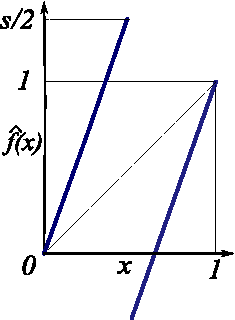
\includegraphics[width=0.30\textwidth]{fig_d_1CL18}
  \caption{\label{fig-d-1f}
$\hflow{}{\ssp}$, the full space sawtooth map \refeq{KD-mapCL18}, ${s} >
2$.
            }
\end{figure}
%%%%%%%%%%%%%%%%%%%%%%%%%%%%%%%%%%%%%%%%%%%%%%%%%%%%%%%%%%%%%%%%%%
%
The closely related {\em sawtooth map}, sketched in \reffig{fig-d-1f},
with `stretching' parameter $s>2$,
\index{sawtooth map}
\beq
\hx_{\zeit+1}
    \,=\, \hflow{}{\hx_{\zeit}}
    \,=\,\left\{
\begin{array}{ll}
{s} \hx_{\zeit}\,,          & \hx_{\zeit} \in [0,{1/2}) \\
{s} \hx_{\zeit} +1 - {s}\,, & \hx_{\zeit} \in ({1/2},1]
\end{array}
\right.
%\,,\qquad {s} \in \{2,3,4, \cdots\}
%\,,
\label{KD-mapCL18}
\eeq

 Since the relation between $\Ssym{\zeit}$ symbol
sequences and $\ssp_{\zeit}$ states is linear, it is straightforward  to
go back and forth between a {\lattstate} and its symbolic
representation.

%%%%%%%%%%%%%%%%%%%%%%%%%%%%%%%%%%%%%%%%%%%%%%%%%%%%%%%%%%%%%
\begin{figure}
  \centering
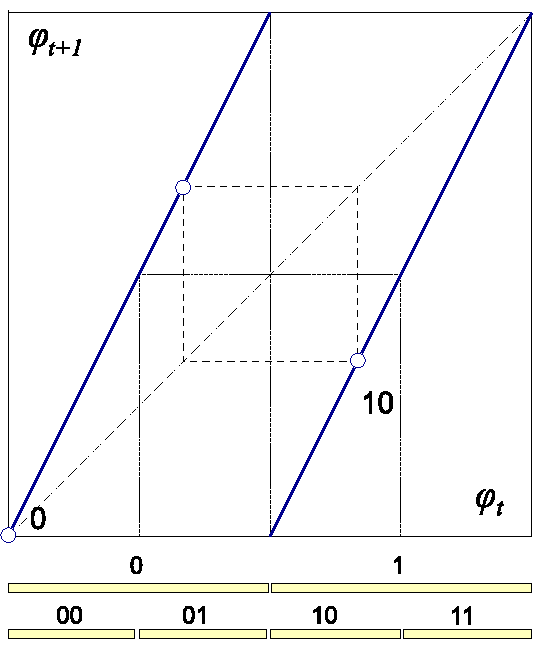
\includegraphics[width=0.35\textwidth]{BernPartKitten}
  \caption{\label{fig:BernPart}
The Bernoulli map \refeq{KD-mapCL18} for ${s}=2$, %{BerShift},
together with the
$\cycle{0}$ fixed point, and the \cycle{01} 2-cycle. Preimages
of the critical point $\ssp_c=1/2$ partition the unit interval into
$\{\pS_0,\pS_1\}$, $\{\pS_{00},\pS_{01},\pS_{10},\pS_{11}\}$, $\dots$,
subintervals.
As the map is a
circle map, $\ssp_{5}=1=0=\ssp_{0} \quad(\mbox{mod}\;1)$.
          }
\end{figure}
%%%%%%%%%%%%%%%%%%%%%%%%%%%%%%%%%%%%%%%%%%%%%%%%%%%%%%%%%%%%%%

The $n$th
preimages $b^{-(n-1)}(\ssp)$ of the critical point $\ssp_c=1/2$
partition the \statesp\ into $2^n$ subintervals, each labeled
by the first $n$ binary digits of points $\ssp=.\Ssym{1}
\Ssym{2} \Ssym{3} \ldots $ within the subinterval:
\reffig{fig:BernPart} illustrates such 4-intervals \statesp\
partition $\{\pS_{00},\pS_{01},\pS_{11},\pS_{10}\}$  for
$\cl{}=2$.

known as the {\em doubling} map if ${s}=2$,
    \index{doubling map}\index{circle map}
\beq
\ssp_{\zeit+1} = 2 \ssp_{\zeit} \;\; (\mbox{mod}\;1)
%    \,,\qquad \qquad \ssp_{\zeit}\in [0,1)
\,,
\ee{DoublingMap}
and {\em ${s}$-tupling} map, \reffig{fig-d-1}\,(b), for
integer stretching parameter ${s}\geq3$,

The relation is linear, and a given \brick\ $\Mm$, or `code' in terms of
alphabet  \refeq{base-sAlph}, corresponds to a unique temporal {\lattstate} $\Xx$ given by the lattice Green's function
\beq
\Xx
= \gd\,\Mm
\,,\qquad
\gd = - \frac{\shift}{\shift - s\,\id}
\,,
\ee{appe:tempBernGreen}
provided we specify the boundary conditions ({\bcs}) for the {\shiftOp}
$\shift$.

The power of the linear encoding of the {temporal
Bernoulli} condition \refeq{1stepDiffEq} is that the
\emph{integer}-valued symbols $\Ssym{\zeit}$ from the finite alphabet
\refeq{base-sAlph} encode the \emph{real-valued} lattice site states
$\ssp_{\zeit}$.

For the  %\rf{GroFuj,art91},
piecewise linear map of \reffig{fig:BernPart}
we can evaluate the \dzeta\ in closed form.
Each branch has the same value of the
slope, and the map can be parameterized
by the single parameter ${s}$.
The larger ${s}$ is, the stronger is the stretching action of the map.

The power of the code % $\{\Ssym{\zeit}\}$
\beq
\transp{\Mm} % = \{\ssp_j\}
             = (\Ssym{\zeit},\Ssym{{\zeit+1}},\cdots,\Ssym{{\zeit+k}})
\ee{linCode}
for the {\templatt} \refeq{OneCat} is that one can use \emph{integers}
$\Ssym{\zeit}$ to encode the \emph{real-valued} {\lattstate}s $\ssp_{\zeit}$.

,
\beq
(\partial - (s-1)\,\shift^{-1})\,\Xx = -\Mm
\,.
\ee{app:1stepVecEq}

For
the $s=3$ cat map example at hand, they are
\beq
\{M_j\} = (M_1,M_2,M_3,M_4,M_5,\cdots)
=(1,2,5,10,24,\cdots)
\,,
\ee{noPrimeCycs=3}

Visualizing the volume relation \refeq{eq:fundFact} for a general \cl{}\dmn\
{\fundPip} is not easy, but

As the {temporal Bernoulli} \refeq{tempBern} is linear, eigenmodes of
$\jMorb$, shifted by $\Mm$ as in \refeq{tempBern} for each distinct
{\lattstate}, are also {\lattstate}s of {temporal Bernoulli}.


    \HLpost{2020-01-17}{
The determinant of this $\jMorb$ from \refeq{tempBern} is negative so
we cannot use the determinant trace formula directly. A correct way is:
first rewrite the $\jMorb$ as in \refeq{appe:tempBernGreen}
\[
\jMorb = \id-{s}{\shift}^{-1}
       = - \frac{s}{\shift} \left(\id-\frac{\shift}{s}\right)
\, .
\]
Note that $\det(\shift)=(-1)^{\cl{}-1}$. The determinant of $\jMorb$ is:
\[
\det \jMorb = \det(\frac{\shift}{s}-\id) s^{\cl{}}(-1)^{\cl{}-1}
   = - s^{\cl{}} \det(\id-\frac{\shift}{s}) \, .
\]
Then use the determinant-trace formula:
\[
\ln\det(\id-\frac{\shift}{s}) = \tr\ln({\id- {\shift}/{s}})
  =
-\sum_{k=1}^\infty\frac{1}{k}\frac{\tr(\shift^k)}{s^k}
\, ,
\]
and use
$\tr \shift^k= \cl{}\delta_{k,\cl{}r}$ if $k$ is a multiple of $\cl{}$,
0 otherwise
(follows from $\shift^\cl{}=\id$),
\[
\ln\det(\id-\frac{\shift}{s}) = -\sum_{r=1}^\infty\frac{1}{r}\frac{1}{s^{\cl{}r}}
=
\ln(1-s^{-\cl{}})
\, ,
\]
and the determinant of $\jMorb$ is:
\[
\det \jMorb = - s^{\cl{}} \det(\id-\frac{\shift}{s}) = 1 - s^{\cl{}}
\, ,
\]
which is negative. So for the {temporal Bernoulli} the count is:
\[
N_\cl{} = |\det \jMorb| = s^{\cl{}} - 1
\, ,
\]
in agreement with the time-evolution count \refeq{noPerPtsBm}.
}

\item[2020-01-25 Predrag:] {\bf A Bernoulli map example}.
%%%%%%%%%%%%%%%%%%%%%%%%%%%%%%%%%%%%%%%%%%%%%%%%%%%%%%%%%%%%%%%%%%%%%%%
% BernCyc2Jacob.svg
% derived from CatMapStatesp.svg
\begin{figure}
  \centering
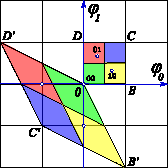
\includegraphics[width=0.45\textwidth]{BernCyc2Jacob}
  \caption{\label{fig:BernCyc2Jacob}
(2020-02-14 Predrag: his is ``wrong'', now superseded with the updated
figure in \refref{CL18}; 2020-09-11 the whole example seems misplaced
here, moce it to wherever it belongs)
The base-2 Bernoulli map \refeq{circ-m=2} period-2 periodic points
$\Xx_p=(\field_0,\field_1)$ are $\cycle{0}=(0,0)$, $\cycle{1}=(1,1)$ fixed
point repeats, and the 2-cycle $\Xx_{01}=({1}/{3},{2}/{3})$,
see \reffig{fig:BernPart}.
They all lie within the unit square $[0BCD]$, one within each
$\pS_{\Ssym{0}\Ssym{1}}$ subregion, and are mapped by the
$[2\!\times\!2]$ {\jacobianOrb} $\jMorb$
% \refeq{jacobianOrb}
into the parallelogram $[0B'C'D']$, whose area is 4 times the unit area.
The images of periodic points $\Xx_p$ land on the integer lattice, and
are sent back into the origin by integer translations $\Mm_p$, in order
to satisfy the fixed point condition
%\refeq{tempBernFix},
$\jMorb\Xx_p+\Mm_p=0$.
          }
\end{figure}
%%%%%%%%%%%%%%%%%%%%%%%%%%%%%%%%%%%%%%%%%%%%%%%%%%%%%%%%%%%%%%
%
The action of {\jacobianOrb}
$\jMorb$ for the period-2 periodic points of the base-2 Bernoulli map,
\reffig{fig:BernPart},
which partitions the unit interval into ${2}$ subintervals
$\{\pS_\Ssym{}\}$, is
\beq
\field_{\zeit+1}
= {2} \field_{\zeit} - \Ssym{\zeit+1}
\,,\qquad  \field_{\zeit}\in\pS_{\Ssym{\zeit}}
\,,
\ee{circ-m=2}
where $\Ssym{\zeit}$ takes values in the ${2}$-letter alphabet
\beq
\Ssym{} \in \A=\{0,1\}
\,.
\ee{base-sAlph=2}

should suffice to convey the idea. In this
case, the $[2\!\times\!2]$ {\jacobianOrb}, the unit
square basis vectors, and their images are
\bea
\jMorb &=&
 \left(\begin{array}{cc}
  1 & -2 \\
 -2 &  1
 \end{array} \right)
;\quad
\Xx_B =
 \left(\begin{array}{c}
 1  \\
 0
 \end{array} \right)
\,,\quad
\Xx_D =
 \left(\begin{array}{c}
 0  \\
 1
 \end{array} \right)
\continue
\Xx_{B'}  &=& \jMorb\,\Xx_B =
 \left(\begin{array}{c}
  1  \\
 -2
 \end{array} \right)
\,,\quad
\Xx_{D'} =
 \left(\begin{array}{c}
-2  \\
 1
 \end{array} \right)
\,,
\eea
with the resulting fundamental parallelogram of area 4
shown in \reffig{fig:BernCyc2Jacob}.
The volume of the fundamental parallelogram lattice $\lattice$ \refeq{lattVol} is
\beq
\Det(\lattice) = \Det(\Xx_{B'}|\Xx_{D'})= \Det(\jMorb)\,\Det(\Xx_{B}|\Xx_{D}) = - 3
\,,
\ee{bernVol}
where in this case the unit cell matrix $(\Xx_{B}|\Xx_{D})=\unit$.


The $[3\!\times\!3]$ {\jacobianOrb} and the unit
cube basis vectors are
\bea
- \jMorb &=&
 \left(\begin{array}{ccc}
  -1  & 0 & 2 \\
  2 &  -1 & 0\\
  0 & 2 & -1
 \end{array} \right)
\,,\quad
\left(\Xx_B|\Xx_C|\Xx_D\right) =
 \left(\begin{array}{ccc}
 1 & 0 & 0\\
 0 & 1 & 0\\
 0 & 0 & 1
 \end{array} \right)
\,.
\nnu
\eea
Clearly $\Det(-\jMorb)= {s}^3-1$, and so on, reproducing the periodic
states count for Bernoulli. No point of looking at $\Det(-\jMorb)$, as
that changes sign at every order - always evaluate $|\Det(\jMorb)|$.

%%%%%%%%%%%%%%%%%%%%%%%%%%%%%%%%%%%%%%%%%%%%%%%%%%%%%%%%%%%%%%%%%%%%%%%
% BernCyc2Jacob.svg
% derived from CatMapStatesp.svg
\begin{figure}
  \centering
{(a)}
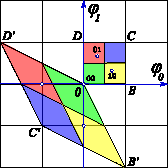
\includegraphics[width=0.35\textwidth]{BernCyc2Jacob}
~~~
{(b)} %$\!\!\!\!$
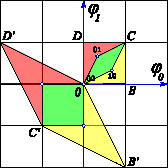
\includegraphics[width=0.35\textwidth]{BernCyc2JacobUnit}
  \caption{\label{fig:BernCyc2JacobOld}
[OLD VERSION] The Bernoulli map \refeq{BerShift} period-2 {\lattstate}s
$\Xx_\Mm=(\ssp_0,\ssp_1)$ are the $\cycle{0}=(0,0)$ fixed
point, and the 2-cycle $\Xx_{01}=({1}/{3},{2}/{3})$, see
\reffig{fig:BernPart}. They all lie within the unit square $[0BCD]$,
one within each $\pS_{\Ssym{0}\Ssym{1}}$ subregion, and are mapped by the
$[2\!\times\!2]$ {\jacobianOrb} $\jMorb$ \refeq{bernFundPar} into the
{\fundPip} $[0B'C'D']$. The images
of periodic points $\Xx_\Mm$ land on the integer lattice, and are sent back
into the origin by integer translations $\Mm$, in order to satisfy the
fixed point condition refeq\{tempFixPoint\}, $\jMorb\Xx_\Mm+\Mm=0$.
\refFig{fig:BernPart} suggests subdividing the {\fundPip}
into (a) 4 areas, but they are not unit areas. The theory of integer lattices
dictates instead (b) covering the {\fundPip} by 3 unit area
rectangles, with
all vertices on the integer lattice.
          }
\end{figure}
%%%%%%%%%%%%%%%%%%%%%%%%%%%%%%%%%%%%%%%%%%%%%%%%%%%%%%%%%%%%%%
%

\PCpost{2020-02-16}{
Dropped from CL18\rf{CL18}:\\
The temporal Bernoulli lattice Green's function %\refeq{appe:tempBernGreen}
in the matrix form
\beq
\gd
=  \left(\begin{array}{ccccccc}
0&\ExpaEig^{-1}&\ExpaEig^{-2}&\ExpaEig^{-3}&\ExpaEig^{-4}&\ExpaEig^{-5}&\cdots\cr
0&  0          & \ExpaEig^{-1}&\ExpaEig^{-2}&\ExpaEig^{-3}&\ExpaEig^{-4}&\cdots\cr
0&  0          &   0          &\ExpaEig^{-1}&\ExpaEig^{-2}&\ExpaEig^{-3}&\cdots\cr
0&  0          &   0          &     0       & \ddots      &  \cr
0&  0          &   0          &     0       & 0           & \ExpaEig^{-1}&\cdots\cr
0&  0          &   0          &     0       & 0           & 0            &\ddots\cr
\vdots&\vdots  &   \vdots     &     \vdots  & \vdots      & \vdots        &\ddots
          \end{array} \right)
\,,
\ee{BernGreenMatrix}
for an infinite temporal Bernoulli
lattice $\zeit\in\integers$, where $\ExpaEig={s}$ is the 1-time step stability
multiplier for the Bernoulli system.
}

\item[2020-02-18 Predrag] Clipped here from
\emph{Ising.tex}, might be relevant to generalizing
Bernoulli to 2\dmn\ lattice, as a warm-up to \catlatt\ zeta functions:

Roettger\rf{Roettger05},
{\em Periodic points classify a family of Markov shifts}, writes:

Ledrappier introduced the following type of space of doubly indexed
sequences over a finite abelian group G,
\[
X_G=\{(x_{s,t}) \in G^{\integers^2} | x_{s,t+1}=x_{s,t}+x_{s+1,t}
\quad \mbox{for all }s,t\in \integers\}.
\]
The group $\integers^2$ acts naturally on the space $X_G$ via left and
upward shifts.

\item[2020-02-19 Predrag]
Suarez\rf{Suarez89}
{\em Difference equations and a principle of double induction},
\CBlibrary{Suarez89}
studies this as a ``partial difference equations,'' that is, difference
equations in two or more variables. He refers to many books on the
subject. His example is a first order hyperbolic equation, with initial
conditions on space and time axes, which describes some thermal
properties,
\[
f(r, m) =f(r, m-1) +f(r-1, m).
%\label{Suarez89(9)}
\]
The goal is to calculate, step by step, all the values of the temperature
T(m,n), starting with the initial and boundary conditions. But then I do
not get the rest of the papers. Perhaps best not to use much time on
`\spt' Bernoulli.

    \item[2020-03-28 Predrag]
The Bernoulli % equation \refeq{circ-m}
first-order difference equation
\beq
\field_{\zeit} - {s}\field_{\zeit-1} = - \Ssym{\zeit}
\,,\qquad  \field_{\zeit} \in [0,1)
\,,
\ee{diffEqs:1stepDiffEq}
{characteristic equation} (for \Ssym{\zeit}=0)
\beq
\ExpaEig -s= 0
\,,
\ee{diffEqs:tempBern}
has one characteristic root
\(
\{s\}
\,.
\)

Comparing with \refeq{genFuncts:noPerPtsBms} we see that we need to solve
a first-order inhomogeneous difference equation with a constant forcing
term $(s-1)$.

Weijie Chen does this pedagogically in his 2011 lecture notes
\CBlibrary{Chen11}, sect.~{\em 1.2.1 One Example}, where he
considers
\beq
\field_{\zeit} - {s}\field_{\zeit-1} = {M}
\,,
\ee{Chen11:1stepDiffEq}
and finds the particular solution by taking
$\field_{p,n} = \field_{p}$ for all $n$,
\[
  \field_{p}-s\,\field_{p}={M}
  \quad \to \quad
  \field_{p} = -{M}/(s-1)
\,.
\]
Hence the solution is
\beq
\field_{n} = \field_{c,n} + \field_{p,n}
= c\,s^{n} - \frac{{M}}{s-1}
\,,
\ee{Chen11:1stepDiffSolu}
with $c$ determined by the initial value
\(
\field_{0}= c\,{s}^{0} - {{M}}/(s-1)
\,.
\)
Bernoulli starts with $\field_{0}=0$, and according to
\refeq{genFuncts:noPerPtsBms}, $M=(s-1)$, so $c=1$.

Weijie Chen also works out the particular solution when $s=1$.
                                    \toCB
He also remarks that in econometrics the {\shiftOp} $\shift$ is called
the \emph{lag operator}.

%\item[2020-03-28 Predrag]
Weijie Chen solves the \templatt\ pedagogically in his lecture notes
\CBlibrary{Chen11}, sect.~{\em 2 Second-Order Difference Equation}.

Questions
\begin{itemize}
  \item
Why is it OK to take site-independent particular solution?
  \item
${{M}}/(s-1)$ looks awkward, can one reformulate? so instead of $M$, have
${{M}}/(s-1)\to1$
  \item
I am guessing that $M=(s-1)$ in \refeq{Chen11:1stepDiffEq}
something like the total number of `letters' I can add to
the count $N_n$ at time $n$. Something like that.
  \item
Similarly for $M=2{\mu}^2$ forcing term in \templatt\ second-order
difference equation \refeq{genFuncts:CatRec-s}.
  \item
This is still just a verification of my guess recurrence
\refeq{genFuncts:noPerPtsBms}.
Make this argument into a derivation.
\end{itemize}

    \PCpost{2020-02-23}{
Just curious - what does the Bernoulli {\fundPip} defined by the columns
of $[3\!\times\!3]$ {\jacobianOrb}
\beq
\jMorb =
\left(
\begin{array}{ccc}
  1 & -2 &  0 \\
  0 &  1 & -2 \\
  -2&  0 &  1
\end{array}
\right)
\,,
\qquad
N_3 = |\Det \jMorb|
    = 2^3-1
\,,
\label{bernFundPar3}
\eeq
look like in a 3\dmn\ rendition? Hopefully it is not symmetric, like
\reffig{fig:catCycJacob}\,(b).
    }

\item[2020-03-01 Predrag]
Wilf\rf{Wilf94} {\em Generatingfunctionology} starts out in his sect.
1.1~{\em An easy 2-term recurrence}, with our Bernoulli periodic points
count \refeq{genFuncts:noPerPtsBm} and
\refeq{genFuncts:1stepDiffEq} as a trivial example of a two-term
recurrence (first-order difference equation).

\item[2020-12-21 Predrag]
{\bf Counting {temporal Bernoulli} {\lattstate}s}
%\label{s:bernCount}
removed from CL18.tex $\to$ Bernoulli.tex, replaced by  refsect{s:Hill1stOrd}
\bigskip

To evaluate the {\HillDet} \refeq{eq:fundFact}, observe that
from \refeq{tempBern} it follows that
\[
\Det(-\jMorb)=\Det({s}/\shift)\,\Det(\id- {\shift}/{s})
\,,
\]
where $|\Det({s}/\shift)|=s^n$. Expand $\ln\Det(\id- {\shift}/{s}) =
\Tr\ln(\id- {\shift}/{s})$ as a series in $1/s$,
\beq
\Tr\ln\left(\id- \frac{\shift}{s}\right)
  =
-\sum_{k=1}^\infty\frac{1}{k}\frac{\Tr(\shift^k)}{s^k}
\,.
\ee{LnDet=TrLn}
It follows from $\shift^\cl{}=\id$ that
$\Tr \shift^k= \cl{}\delta_{k,r\cl{}}$ is non-vanishing
if $k$ is a multiple of $\cl{}$,
0 otherwise:
\[
\ln\Det(\id- {\shift}/{s})
  =
-\sum_{r=1}^\infty\frac{1}{r}\frac{1}{{s}^{\cl{}r}}
  =
\ln(1-{s}^{-\cl{}})
\,.
\]

\item[2020-12-09 Predrag]
{\bf Temporal Bernoulli}
% \label{appe:1D1dLatt}
% was file siminos/kittens/appeBernoulli.tex      pdflatex CL18
%\renewcommand{\statesp}{state space}
%\renewcommand{\Statesp}{State space}
%\renewcommand{\stateDsp}{state-space}
%\renewcommand{\StateDsp}{State-space}
\index{cyclic!permutation matrix}

After $\cl{}$ shifts, the {\lattstate} \Xx\ returns to the initial
state, $\shift^\cl{}=\id$. This relation leads to the explicit expression for
the orbit {\jacobianM} \refeq{appe:tempBernGreen},
\beq
\gd
    =  \frac{\shift}{s\,\id-\shift}
    = \frac{1}{\id-\frac{\shift}{s}}\,\frac{\shift}{s}
    = \sum_{k=1}^\infty \frac{\shift^k}{s^k}
%    =  \sum_{m=0}^\infty \frac{1}{s^{\cl{}m}}
%      \sum_{k=1}^\cl{} \frac{\shift^k}{s^k}
    =  \frac{s^\cl{}}{s^\cl{} - 1}
      \sum_{k=1}^\cl{} \frac{\shift^k}{s^k}
\,.
\ee{appe:BernGreenFct}
From \refeq{appe:tempBernGreen} it then follows that the last field in
$\Xx$ is the field at lattice site $\cl{}$
\beq
\ssp_{\cl{}}
=  \frac{s^\cl{}}{s^\cl{} - 1}
          .\Ssym{1}\Ssym{2}\Ssym{3}\cdots\Ssym{\cl{}}
=  \frac{1}{s - 1}\,%\sum_{k=1}^\cl{} \Ssym{k} 2^{\cl{}-k}
    \frac{s^{\cl{}-1}\Ssym{1}+\cdots+s\,\Ssym{\cl{}-1}+\Ssym{\cl{}}}
         {s^{\cl{}-1}+\cdots+s+1}
\,,
\label{appe:Bern_cyc}
\eeq
and the rest are obtained by cyclic permutations of $\Mm$.

% from ChaosBook \Chapter{appendKnead}
% \section{Pruned Bernoulli shift} \label{sect:PrunBernoulli}
For example, for ${s}=2$, the lattice fields are (they are always rational-valued),
\bea
\ssp_{\Ssym{1}\Ssym{2}\cdots \Ssym{n}}
&=&  \sum_{k=1}^\cl{} \frac{\Ssym{k}}{2^k} \sum_{m=0}^\infty \frac{1}{2^{\cl{}m}}
        = \frac{2^\cl{}}{2^\cl{} - 1} .\Ssym{1}\Ssym{2}\cdots \Ssym{\cl{}}
\continue
&=& \frac{1}{2^\cl{} - 1}\,\sum_{k=1}^\cl{} \Ssym{k} 2^{\cl{}-k}
\,,
\label{Bern_cyc1}
\eea
where $p=\overline{\Ssym{1}\Ssym{2}\cdots \Ssym{\cl{}}}$ is an {\orbit} of period
\cl{}, with stability multiplier $\ExpaEig_p=2^\cl{}$.

For a Bernoulli map,
the rational $\ssp_{0}$ are either periodic or land eventually on a \po\
(the base-${s}$ version of the familiar fact that the decimal expansion
of a rational number is eventually periodic), while the orbit of a normal
irrational $\ssp_{0}$ is ergodic.

    \item[2020-12-09, 2020-12-11 Predrag]
Quotienting the temporal Bernoulli system
\beq
\ssp_{\zeit} - {s}\ssp_{\zeit-1} = - \Ssym{\zeit}
\,,\qquad  \ssp_{\zeit} \in [0,1)
\,,
\ee{1stepDiffEqBlog}
by its \emph{dynamical} $\Dn{1}=\{e,\Refl\}$
symmetry
\beq
\Refl \ssp_\zeit = 1-\ssp_\zeit
    \,,\quad
\Refl \Ssym{\zeit} = (s-1)-\Ssym{\zeit}
    \,,\qquad
\mbox{ for all } \zeit\in\integers
\,,
\ee{BernDynD1}
where $\Ssym{\zeit}$ takes values in the ${s}$-letter alphabet
\beq
\Ssym{} \in \A=\{0,1,2,\cdots,s-1\}
\,.
\ee{base-sAlphBlog}
Define the fundamental domain to be ${\sspRed}_\zeit\in[0,1/2]$.
We construct the
Bernoulli fundamental domain lattice system, with `1/2' unit hypercube
$\hat{\Xx}\in[0,1/2]^\cl{}$, as in
\toChaosBook{exmple.11.3}
{{\em Group \Dn{1} and reduction to the fundamental domain}},
see \reffig{fig:fig_d_2half}\,(b),
and the fundamental domain symbolic dynamics $\hat{\A}$.
The temporal lattice Bernoulli condition \refeq{1stepDiffEqBlog} is now
two conditions  (Bernoulli)/$\Dn{1}$.
They are different for ${s}$ even or odd:
\bea
{\sspRed}_{\zeit+1} - {s} {\sspRed}_{\zeit} &=&
            - \Ssym{\zeit+1}
\,,\qquad  {\sspRed}_{\zeit}\in\pS_{\Ssym{\zeit}}
\,,\quad {s} \mbox{ even}
    \continue
{\sspRed}_{\zeit+1} + {s}{\sspRed}_{\zeit} &=&
       1 + \Ssym{\zeit+1}
\,,\qquad  {\sspRed}_{\zeit}\in\pS_{\Refl\Ssym{\zeit}}
    \label{circ/D1}\\
% \hat{\Ssym{}} \in
\hat{\A}~~~~ &=& \{\{\Ssym{}\},\{\Refl\Ssym{}\}\}
\,,\;\; \{\Ssym{}\} = \{0,1,2,\cdots,{s}/2\}
\,,
\nnu
\eea

\bea
{\sspRed}_{\zeit+1} - {s} {\sspRed}_{\zeit} &=&
\,,\;\;    {s} \mbox{ odd}
\label{base-sRed}\\
%\hat{\Ssym{}} \in
\hat{\A} &=&
\{\{\Ssym{}\},({s}-1)/2,\{\Refl\Ssym{}\}\}
\,,\;\;     \Ssym{}\in \{0,1,2,\cdots,(s-3)/2\}
\,.
\nnu
\eea
As an example, case
${s}=6$,
$\Ssym{\zeit}\in\{0,1,2\}$
is worked out in \reffig{fig:fig_d_2half}\,(c).
(Plot also the fundamental domain map for odd values of ${s}$.)
%
%%%%%%%%%%%%%%%%%%%%%%%%%%%%%%%%%%%%%%%%%%%%%%%%%%%%%%%%%%%%%
\begin{figure}
  \centering
{(a)}
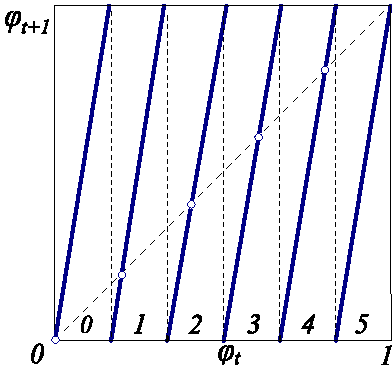
\includegraphics[width=0.40\textwidth]{fig_d_2kitten}
~~~
{(b)}$\!\!\!\!$
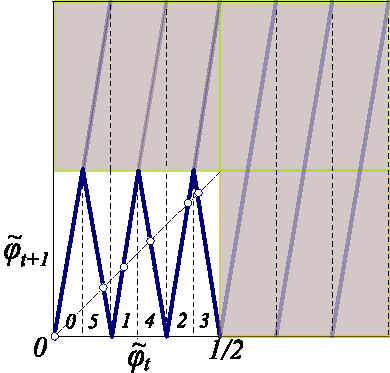
\includegraphics[width=0.40\textwidth]{fig_d_2half}
\\ %~~~
{(c)}$\!\!\!\!$
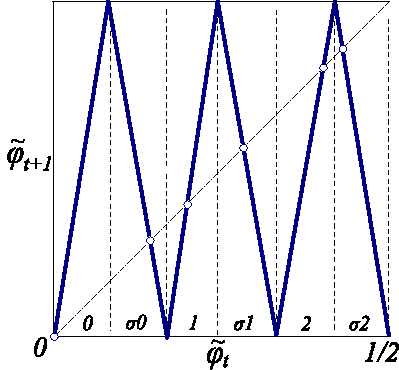
\includegraphics[width=0.40\textwidth]{fig_d_2fund}

  \caption{\label{fig:fig_d_2half}
(a)
The Bernoulli map $f$ with the  stretching parameter ${s}=6$
partitions the unit interval into $6$ subintervals $\{\pS_{\Ssym{}}\}$,
labeled by the ${6}$-letter alphabet \refeq{base-sAlphBlog}. As the map is a
circle map, $\ssp_{5}=1=0=\ssp_{0} \quad(\mbox{mod}\;1)$.
(b)
The Bernoulli map is quotiented by the
\emph{dynamical} $\Group=\Dn{1}=\{e,\Refl\}$
symmetry to
(c)
the fundamental domain ${\sspRed}_\zeit\in[0,1/2]$ map
$\hat{f}=f/\Group$ partitions the half interval into the three $1/12$
subintervals $\{\pS_{0},\pS_{1},\pS_{2}\}$, and their reflections, the
three $3$ subintervals $\{\pS_{\Refl0},\pS_{\Refl1},\pS_{\Refl2}\}$,
labeled by a ${6}$-letter reduced system's alphabet. Reduced space
fixed points $\{\cycle{\Refl_0},\cycle{\Refl_1},\cycle{\Refl_2}\}$
correspond to self-dual 2-cycles
$\{\cycle{05},\cycle{14},\cycle{23}\}$
in the full space. Fixed point $\cycle{0}$ is in the border,
and thus over-counted;
$\cycle{1}$ corresponds to $\{\cycle{1},\cycle{4}\}$, and
$\cycle{2}$ corresponds to $\{\cycle{2},\cycle{3}\}$.
          }
\end{figure}
%%%%%%%%%%%%%%%%%%%%%%%%%%%%%%%%%%%%%%%%%%%%%%%%%%%%%%%%%%%%%%
%

In the matrix form \refeq{1stepDiffEqBlog}, the {\jacobianOrb}
\beq
\jMorb\,\Xx = - \Mm
\,,\qquad
\jMorb = \unit-{s}{\shift}^{-1}
% former \ee{tempBernFix}
\,,
\ee{HLtempBern}
is independent of $\Mm$. Not so for the symmetry reduced  {\jacobianOrb}
${\MvarRed}_{\hat{\Mm}}$ in \refeq{circ/D1}: it depends on
$\hat{\Mm}$, as its diagonal takes values $\pm{s}$. We need to prove
that the \HillDet\ $\Det{\MvarRed}$ does not.

I had not noticed before that this parametrization converts
Bernoulli into tent map, with full \statesp\ 2-cycles turned
into negative slope fixed points.

By the
inclusion-exclusion principle \refeq{KlaRot97(2.1)}
\beq
N_\cl{}=
  \hat{N}_\cl{}+\Refl\hat{N}_\cl{}-\hat{N}_\cl{}\cap(\Refl\hat{N}_\cl{})
      =
  2\hat{N}_\cl{}-\hat{N}_\cl{}\cap(\Refl\hat{N}_\cl{})
\,.
\ee{Bern:inclExcl}
Let's call the number of points in the shared boundary $I$.
% Looks like we have to distinguish odd and even $\cl{}$.
The $\ssp=0$ is in $I$
for any $\cl{}$, if I am allowed to identify $\ssp=1\to0$,
and that is the only point in the boundary.
Presumably this leads to the denominator $(1-z)$ in
\refeq{appe:BernZeta}. I guess that the symmetric irrep of
$\Dn{1}=\{e,\Refl\}$ leads to $N_{+}=s^\cl{}$ and the numerator
$(1-{s}z)$, while the antisymmetric irrep leads to $N_{-}=0$, and a
trivial factor 1 contribution to the numerator \refeq{appe:BernZeta}.
\bea
\zetatop(z)
 &=&
\frac{1 -  {s}z}{1 - z}
\,.
\label{appe:BernZeta}
\eea

\tempLatt\ should be more interesting. Also any nonlinear $s$-branch map
`Bernoulli-like' lattice with a \emph{dynamical} $\Dn{1}$ symmetry; then
the weights $t_p$ do not necessarily cancel for the antisymmetric irrep.

\item[2018-12-27 Linas Vepstas]
{\em On the Beta Transformation} \arXiv{1812.10593}:
The beta transformation is the iterated map \refeq{betaTransf}. The
$\beta=2$ is known as the Bernoulli map, and is exactly solvable. The Bernoulli
map provides a model for pure, unrestrained chaotic (ergodic) behavior:
it is the full invariant shift on the Cantor space. The beta
transformation defines a subshift: iterated on the unit interval, it
singles out a subspace of the Cantor space, in such a way that it is
invariant under the action of the left-shift operator. That is, lopping
off one bit at a time gives back the same subspace. The beta transform
seems to capture something basic about the multiplication of two real
numbers: $\beta$ and $x$. It offers a window into understanding the nature of
multiplication. Iterating on multiplication, one would get
exponentiation; although the mod 1 of the beta transform contorts this in
interesting ways. The work presented here is a research diary: a pastiche
of observations and some shallow insights.
 The eigenvalues of the
transfer operator seem to lie on a circle of radius $1/\beta$ in the complex
plane. Given that the transfer operator is purely real, the appearance of
such a quasi-unitary spectrum seems surprising. The spectrum appears to
be the limit of a dense set of quasi-cyclotomic polynomials, the positive
real roots of which include the Golden and silver ratios, the Pisot
numbers, the n-bonnaci (tribonacci, tetranacci, etc.) numbers.

Beta transformation
\beq
T_{\beta }(x)=\beta x\;{\mod {1}}
\,,\qquad 1<\beta\leq2
\ee{betaTransf}
was introduced by Alfr{\'e}d R{\'e}nyi\rf{Renyi57} in 1957, and an invariant measure for
it was given by Alexander Gelfond in 1959 and independently by Bill
Parry\rf{Parry60} in 1960.

\HREF{https://arxiv.org/pdf/1812.10593.pdf\#subsection.1.9}
{Beta transformation literature review and references}.

\HREF{https://mathoverflow.net/questions/265916/concise-introduction-to-beta-transformations}
{{\em A concise intro to beta-transformations?}} has references.

% A. O. Gel’fand, “A common property of number systems”,
%           Izv Akad Nauk SSSR Ser Mat, 23, 1959, pp. 809–814.

% P. Gaspard, "r-adic one-dimensional maps and the Euler summation
%           formula", Journal of Physics A, 25 (letter) L483-L485 (1992).


\item[2020-09-08 Predrag]
\HREF{https://sites.google.com/site/homepagebingli}{Bing Li}
{\em Some fractal problems in beta-expansions}
\HREF{https://www.irif.fr/~numeration/OWNS}{(video)}
\HREF{https://www.irif.fr/~numeration/uploads/Main/li_20200908.pdf}{(slides)}

For greedy beta-expansions, we study some fractal sets of real numbers
whose orbits under beta-transformation share some common properties. For
example, the partial sum of the greedy beta-expansion converges with the
same order, the orbit is not dense, the orbit is always far from that of
another point etc. The usual tool is to approximate the
beta-transformation dynamical system by Markov subsystems. We also
discuss the similar problems for intermediate beta-expansions.

\item[2021-01-05 Predrag]
Hofbauer and Keller\rf{HofKel84} {\em Zeta-functions and
transfer-operators for piecewise linear transformations} (1984) has no
Bernoulli zeta. Not useful to us at this time.

\item[2021-01-05 Predrag]
Takahashi\rf{Takahashi81} {\em Fredholm determinant of unimodal linear
maps} has lots of detail and examples. I might have missed something, but
Bernoulli zeta is not there, or anything we care about.

\item[2021-01-04 Predrag]
Flatto, Lagarias and Poonen\rf{FlLaPo94}
{\em The zeta function of the beta transformation} (1994)

which should have the $\beta=2$ Bernoulli zeta function
as the trivial case.

\item[2021-01-05 Han] Notes from Flatto, Lagarias and Poonen\rf{FlLaPo94} paper:

$\beta$-transformation map is:
\[
f_\beta(x) = \beta x \;\; (\mbox{mod}\;1) \, ,
\]
where $\beta>1$, $x \in [0,1]$. The symbolic dynamics of $f_\beta$ is based on the fact that the graph of
$f_\beta$ consists of $\lfloor \beta \rfloor + 1$ monotone pieces which they call laps, which are
assigned by the symbols $0, 1, \dots, \lfloor \beta \rfloor$. When $\beta \in \mathbb{Z}^+$,
the piece $\lfloor \beta \rfloor$ consists of a single point, and the symbol $\lfloor \beta \rfloor$
only appears in the itinerary of 1. To each $x \in [1,0]$ its itinerary is $I_\beta(x)=A_0A_1A_2\dots$,
where the symbol
\[
A_n := A_n(x) = \lfloor \beta f_\beta^n(x) \rfloor \, .
\]
In particular the itinerary of 1, $I_\beta(1)=A^*_0A^*_1A^*_2\dots$ encodes complete information about
the behavior of $f_\beta$.

They introduced a power series with integer coefficients:
\[
\phi_\beta(z) = A_0^* z + A_1^* z^2 + A_2^* z^3+ \dots = \sum_{n=0}^{\infty} A_n^* z^{n+1} \, .
\]
This function is related to the iterates of 1 by:
\[
\phi_\beta(z) = 1 + (\beta z - 1)\left(
\sum_{n=0}^\infty f_\beta^n(1)z^n
\right)
\, .
\]
Then the zeta function is:
\[
\zeta_\beta(z) = \frac{1}{1-\phi_\beta(z)} \, ,
\]
if $\beta$ is not a simple $\beta$-number, and
\[
\zeta_\beta(z) = \frac{1-z^N}{1-\phi_\beta(z)} \, ,
\]
if $\beta$ is a simple $\beta$-number, and $N$ is minimal with $f_\beta^N(1)=0$.
Simple $\beta$-numbers are the $\beta$-numbers such that for some $n$, $f_\beta^n(1)=0$.
This formula gives the correct topological zeta function of temporal Bernoulli.

Associated with the $\beta$-transformation is the set $X_\beta$ of all $I_\beta(x)$ for $0 \leq x <1$.
The $\beta$-shift $S_\beta$ is a symbolic dynamical system obtained as the smallest closed (two-sided)
subshift of $\{1,2,\dots \lfloor \beta \rfloor\}^{\mathbb{Z}}$ generated by all finite substrings of $X_\beta$.
For simple $\beta$-numbers $S_\beta$ is a subshift of finite type.

There is a zeta function associated to the $\beta$-shift $S_\beta$, which is studied by
Takahashi\rf{Takahashi83}, who showed that
\[
\hat{\zeta}_\beta(z) = \frac{1}{1-\phi_\beta(z)} \, .
\]
This formula is closely related to $\zeta_\beta(z)$ but differs from it for simple $\beta$-numbers,
in which case the closure operation defining $S_\beta$ adds some extra periodic points.

\item[2021-01-11 Predrag] Seth Lloyd \etal. %\rf{LDGKLMTP20}
{\em Quantum algorithm for nonlinear differential equations}
\arXiv{2011.06571}:

[1] showed how to map the problem of solving a general linear differential
equation to that of matrix inversion, which can then be performed using
the quantum linear systems algorithm [12-13].   Consider a linear differential
equation of the form,
$$ {dx\over dt} + A x = b(t), \eqno(6)$$
where as above $x,b \in {\cal C}^d$ and $A$ is a $[d\times d]$ matrix.

                                                            \toCB
Discretize the equation in time at intervals $\Delta t$, and take $k$ to
be the index for the discretized time, so that $x_k$ and $b_k$ are
the values of $x$ and $b$ at time label $k$.

We wish to integrate equation
(6) numerically starting from the initial state $x_0 \equiv b_0$.   We obtain
a series of equations of the form:
$$
 x_0 = b_0 \quad
x_1 = x_0 - \Delta t A x_0 + \Delta t b_1 \quad
\ldots \quad
x_{k+1} = x_k - \Delta t A x_k + \Delta t  b_k \quad
\ldots
\eqno(7)$$
Here, we have used the Euler forward method for numerical integration, but it
is straightforward to implement implicit methods such as
Euler backward, Crank-Nicholson, Runge-Kutta, etc.~[3].
Written in matrix form, these equations become
$$-\left(\begin{array}{cccccc}
- I & 0 & 0 & \ldots & 0 & 0 \cr
I-\Delta t A & - I & 0 & \ldots & 0 & 0 \cr
0 & I-\Delta t A& -I &  \ldots & 0 & 0\cr
&&\ldots &&&\cr
0& 0 & 0 & \ldots & - I & 0\cr
0& 0 & 0 & \ldots & I - \Delta t A & - I\cr
          \end{array} \right)
\left(\begin{array}{c}
x_0 \cr x_1 \cr x_2 \cr \ldots \cr x_{T-1} \cr x_{T}
          \end{array} \right)
=
\left(\begin{array}{c}
b_0 \cr \Delta t b_1 \cr \Delta t b_2 \cr \ldots \cr \Delta t
b_{T-1} \cr \Delta t b_{T}
          \end{array} \right)
%\eqno(8)
\,,
$$







\end{description}

%%%%%%%%%%%%%%%%%%%%%%%%%%%%%%%%%%%%%%%%%%%%%%%%%%%%%%%%%%%%%%%%%%%%%%%%%%%%%
\Remarks
%%%%%%%%%%%%%%%%%%%%%%%%%%%%%%%%%%%%%%%%%%%%%%%%
% PC 2021-01-04 eventually merge into
% \Chapter{appendStatM}{22jun2016}{Statistical mechanics applications}
\remark{Bernoulli map.}{\label{rem:Bernoulli}
The Bernoulli shift map \refeq{BerShift} and the doubling map
\refeq{DoublingMap} are also known as the dyadic transformation, dyadic
map, bit shift map, angle doubling map or sawtooth map \refeq{KD-map}.
There are many fine books that discuss it in depth, for example Driebe\rf{Driebe99}.
See also \refrem{rem-GroRue}.
\index{Bernoulli!shift}\index{shift!Bernoulli}
\index{doubling map}\index{circle map}
\index{dyadic transformation}\index{dyadic map}
\index{bit shift map}\index{angle doubling map}
\index{sawtooth map}
    } %end \remark{rem:Bernoulli}
%%%%%%%%%%%%%%%%%%%%%%%%%%%%%%%%%%%%%%%%%%%%%%%%

%%%%%%%%%%%%%%%%%%%%%%%%%%%%%%%%%%%%%%%%%%%%%%%%
% PC 2021-01-04 eventually merge into
% \Chapter{converg}{9nov2008}{Why does it work?}
\remark{Bernoulli shift.}{ \label{rem-GroRue}
For a more in-depth discussion, consult chapter~3 of \refref{Driebe99}.
The extension of Fredholm theory to the case of Bernoulli shift on
$\complex^{k+\alpha}$ (in which the \FPoper\ is {\em not} compact  --
technically it is only {\em quasi-compact}. That is, the essential
spectral radius is strictly smaller than the spectral radius) has been
given by Ruelle\rf{Ruelle90}: a concise and readable statement of the
results is contained in \refref{Baladi95}. We see from \refeq{mixing-BS}
that for the Bernoulli shift the exponential decay rate of correlations
coincides with the Lyapunov exponent: while such an identity holds for a
number of systems, it is by no means a general result, and there exist
explicit counterexamples.
See also \refrem{rem:Bernoulli}.
\index{Bernoulli!shift}\index{shift!Bernoulli}
} %end \remark{Bernoulli shift on $C^{k+\alpha}$}{
%%%%%%%%%%%%%%%%%%%%%%%%%%%%%%%%%%%%%%%%%%%%%%%%

\RemarksEnd

%%%%%%%%%%%%%%%%%%%%%%%%%%%%%%%%%%%%%%%%%%%%%%%%%%%%%%%%%%%%%
\fastTrackExam{exam:BernShad}     % \toExam
%%%%%%%%%%%%%%%%%%%%%%%%%%%%%%%%%%%%%%%%%%%%%%%%%%%%%%%%%%%%%


%%%%%%%%%%%%%%%%%%%%%%%%%%%%%%%%%%%%%%%%%%%%%%%%%%%%%%%%%%%%%%%
%\section{Any piecewise linear map has ``linear code''}
%\label{exam:tentMapSymbDyn}
% siminos/spatiotemp/chapter/tentMapCode.tex
% $Author: predrag $ $Date: 2020-05-07 17:34:06 -0400 (Thu, 07 May 2020) $


%%% input by % siminos/spatiotemp/chapter/catMap.tex %%%%%
\section{Any piecewise linear map has ``linear code''}
\label{exam:tentMapSymbDyn}

                                                            \toCB
For reasons unbeknownst to me, it is below the dignity of any cat to work out
any problem in Chaos\-Book, or in the online course, no matter how often I
point out that it is easier to understand what we do for cat maps if you
first work it out for 1\dmn\ maps.

So I have to do these exercises myself - I'm forced to it, so Li Han can be
motivated to re-derive his polynomials (as described in Bird and
Vivaldi\rf{BirViv}, see my notes of {\bf 2016-05-21, -12-12} below), rather
than to fit them to Mathematica grammar rule counts for integer $s$.

Basically, I am baffled by why should ``linear code'' be such a big deal that
it has to go into the title of our paper\rf{GHJSC16}. {\em Every} example of
symbolic dynamics worked out in Chaos\-Book is a ``linear code.'' The strategy
is always the same - find a topological conjugacy from your map to a
piecewise linear map, and then use the fact that any piecewise linear map has
``linear code.'' The pruning theory is always the same - kneading orbit
separates {\admissible} from the {\inadmissible}, also in the infinite 1\dmn\
discrete lattice case worked out in the {\em Diffusion} chapter in the
Chaos\-Book, and the appendix (\refchap{c-appendStatM} reproduced here) that no
one wants to read either.

A tent map is a 1\dmn\ example (a simpler one would be Bernoulli, and its
sawtooth generalizations). The 2\dmn\ examples are the Belykh map,
\refexam{exam:BelykhLCod}, and the Lozi map, \refexam{exam:LoziLCod}. Belykh map
is of particular interest to us, as it is in form very close to the cat
map. Both maps have the pruning front conjecture is proven for them, for
a some sets of parameters.

%%%%%%%%%%%%%%%%%%%%%%%%%%%%%%%%%%%%%%%%%%%%%%%%%%%%%%%
\hfill    \fastTrackExam{exam:TentLCod}
          \fastTrackExam{exam:TentCycl}

\hfill    \fastTrackExam{exam:BelykhLCod}
          \fastTrackExam{exam:LoziLCod}


\section{Cat map blog}
\label{sect:CatMapBlog}

\begin{description}

    \PCpost{2016-05-18}{                                        \toCB
I start with our 2011 \emph{Notes for cat map}\\
(former \emph{appendStatMnotes.doc} in \emph{dasbuch/book/notes}),\\
to be eventually merged with \emph{chapter/appendStatM.tex}.
    }

\item[2011-05-14 Jean-Luc Thiffeault]
I figured
out that the grouping of \po s is crucial, and moreover that there is
something delicate with the fixed point of the cat map, which lies on the
boundary of Markov boxes.

\item[2011-05-14 Predrag]
For Anosov (linear Anosov?) - Arnol'd cat map - it should work like ton of
rocks, but you have to note that because of the periodicity there is one
fixed point, not two. If you screw up an early term in the series, then
it converges very slowly. I think the Stephen Creagh\rf{Creagh94} tested
it on weakly nonlinearly perturbed cat map (weakly, so golden-mean
grammar is working) and it converged super-exponentially (you know the
grammar, flow has bounded hyperbolicity, so weight-truncated cycle
expansions are not needed - they perform less well).

\item[2011-05-14 Jean-Luc Thiffeault]
I know how to do it with the Markov partition now, and it works much better.
Keep in mind this is a warmup problem: what I really have in mind (with
my collaborator Erwan Lanneau\rf{LanThi11}) is to compute {\po s} for
Teichmuller flow, where the {\po s} themselves are actually now
pseudo-Anosovs!

\item[2011-05-16 Hans-Henrik Rugh]
% Hans-Henrik.Rugh@math.u-cergy.fr
The situation as I recall it is roughly as follows:

When you construct the symbolic dynamics you may start by picking one
\po, typically the fixed point  $p=f(p)$  (but the following
depends on the choice).  You then cut the torus into pieces following
$s/u$-manifolds until you get a small collection of $N$ rectangles.
\[
R_1,\cdots,R_N
\]
Associated to this collection you have a transition matrix (for SINGLE
rectangles).  Now, you also need to construct a transition matrix for
PAIRS of rectangles, e.g.  $(R_1,R_2)  \to  (R_2,R_1)$ and then TRIPLES of
rectangles ... $(R_1,R_2,R_3) \to (R_2,R_1,R_3)$, etc....
These k'th - order transitions comes from the fact that there is a fixed
point/periodic cycle on the boundary of the Markov partition elements.

You get determinants   $d_k(z)$ for each of these k'th–order transition matrices.
 NB :
$(R_1,R_2) \to (R_2,R_1)$  is a \po\ of prime length 2 even if
it represents a fixed point of f. I think (but is not sure?) that the
weights in the determinant are calculated in the same way...

The final determinant is
\(
d(z)=d_1(z)d_3(z)... / (d_2(z) d_4(z)...)
\)
if I am not mistaken. This is related to the so-called Manning trick\rf{manning} for
counting real orbits related to
\[
\det (1 - s) = 1 - \tr s + \tr s \wedge s
- \cdots
\]
where $s$ is a permutation.
What is not obvious is that $d(z)$  is entire, but it is!

%\item[2011-05-18 Hans-Henrik Rugh]
It's a kind of model problem anyway. In more realistic systems I suppose
that one may run into the problem of having several orbits on boundaries.

One of the tricky points is to see how such an orbit in the `higher'
order zeta-functions/Fredholm-det.

As mentioned in e.g. $d_1(z)$ a 'physical' fixed point may appear
zero times, or twice, or,...? In $d_2(z)$ a fixed point may actually appear
as a period two orbit, so should be treated as such when looking for
cancelling terms.

Great, if you have managed to make it work in practice.
I don't think that one can call it a standard trick but one may perhaps
get it implicitly from the paper of Ruelle\rf{Ruelle90}. But it is
difficult to digest and even more difficult to convert into computable
formulae.

    \PCpost{2018-02-10}{
Manning\rf{manning} writes: ``
According to Bowen\rf{Bowen70}, a Markov partition is a finite cover of \statesp\
by closed subsets called \emph{rectangles}. The rectangles are pairwise disjoint
except possibly for the intersection of their boundaries.
[...]
At the boundaries of the rectangles, that is where they intersect,
several periodic points individual rectangles may be mapped to the same periodic
point in the full \statesp.
''

``
Counting the periodic points involves also certain auxiliary subshifts of finite
type to remedy overcounting of points in the boundaries of the rectangles.
''
    }

\item[2011-05-18 Jean-Luc Thiffeault] emailed to Predrag
pdf file {\em Notes on \po\ expansions for Teichm\"uller flow}
(saved as \emph{POexp.pdf} in \emph{dasbuch/book/notes/}).
which maybe figures out cat map symbolic dynamics. He writes:

``
Updated notes: on page 4-5 I used the Markov boxes to compute the PO
expansion.  I used a trick to deal with the orbit on the boundary:
include several copies of the orbit, but divide by the correct factor.
It makes the series very nicely convergent.  I don't know if this is a
standard trick but it seems to work well.
''

    \PCpost{2011-05-17}{
It is standard, it is in ChaosBook.org Chapter {\em Counting}, Sect {\em
Counting cycles}. I introduced it in Roberto Artuso, Erik Aurell and
Predrag Cvitanovi\'c\rf{AACII}, {\em Recycling of strange sets: II.
applications}, see eq.~(4) and Fig.~6, but Manning\rf{manning} did it it
in 1971 (if that's what he did), and Ruelle\rf{Ruelle90} at the same
time, according to Hans Henrik.
Chaos\-Book says: ``Smale\rf{smale_61} conjectured rationality of the zeta
functions for Axiom A diffeomorphisms, later proved by
Guckenheimer\rf{Guckenh77} and Manning\rf{manning}," and Chaos\-Book cannot
be wrong.

The rule of thumb is that all credit should go to old white male
mathematicians whose names one knows how to spell.

The argument is something like this: the correct object, the Fredholm
determinant, can be written as ratios of products of skew products (AKA
determinants of different dimensions), each one being the not correct
object, but historically the first thing written down (dynamical or
Ruelle zeta function).

The ones on partition boundaries (what I currently call `ridges') are of
lower dimensions, either downstairs or upstairs in these rations. They
account for overcounting of the boundary fixed and periodic points.

Chaos\-Book does something of that when explaining the relation between
Fredholm determinants and dynamical zeta functions, but is so far silent
on explicit examples of the Manning multiples. That is why I would really
like us to write up the cat map symbolic dynamics simply and elegantly.
Jean-Luc is not the only person who has gotten lost here, anybody
mathematician who thinks that Arnol'd is the simplest exercise to try
sinks precisely at this spot (physicists train on unimodal maps and the
3-disk system, remaining blissfully ignorant of the Manning multiples)

Hans Henrik might have more elegant way of saying this. Vivianne still more elegant.
    }

    \PCpost{2012-03-01}{
I've been dreaming about this forever, see for example my post
of {\bf [2012-03-01]}, \texttt{pipes} repository,
{\em A letter to our experimental friends}:

``
For large aspect systems I imagine we fit local \template s whose 2\dmn\
or 3\dmn\ volume is concentrated on a region big enough to capture
interaction of close-by structures, but small enough not to track weakly
interacting ones.

In other words, cover 3\dmn\ volume with a finite-size \template\ that
tracks a neighborhood for a finite time. It's OK to make it spatially
periodic, as long as distance is measured in finite size spatiotemporal
windows. That is what we already do when we use unstable \po s - we use
 temporally-infinite periodic solution (that cannot be seen in
experiment) to identify a finite-time neighboring segment of a chaotic
trajectory.

It has not been tried, so I might be wrong (again).
''
    }

    \PCpost{2016-05-04}{
I am not suggesting that we should study this, but it's something to
maybe keep in mind:
Slipantschuk, Bandtlow and Just\rf{SlBaJu16}, {\em Complete spectral data for
analytic {Anosov} maps of the torus}, construct a family of analytic
hyperbolic diffeomorphisms of the torus (of which Arnol'd cat map is a special
case) for which the spectral properties of the associated transfer operator
acting on a suitable Hilbert space can be computed explicitly. They introduce
an example of an analytic hyperbolic diffeomorphism on the complex unit
torus, of which the cat map is a special, linear case. the real
representation of the map, Eq.~(2) is area-preserving and thus provides an
example of a chaotic Hamiltonian system. Unlike  the  situation  for
one-dimensional  non-invertible  maps, here  is  no distinction  between
{\FPoper}s  and  Koopman  operators  as   diffeomorphism is
area-preserving.


Note that the eigenvalues of the evolution (transfer) operators come in
doublets or quadruplets, presumably because of the discrete symmetries of the
unit square.

Just looking at their Figs.~1 is inspirational.

The cat map can always be written as a composition of area preserving
orientation reversing linear automorphisms.
They define a two-parameter area-preserving family, Eq.~(85), and show that
measures for such maps, where the determinant of the Jacobian varies, may have
fractal properties, see Fig.~2.
    }

\item[2016-05-16 PC]
Weirdly, Wolfram's Weisstein\rf{WolframArnCatMap} is wrong: what he calls
\HREF{http://mathworld.wolfram.com/LyapunovCharacteristicExponent.html}
{``Lyapunov characteristic exponents''} for Arnol'd cat map are
certainly not ``exponents'' but multipliers. Maybe you guys could alert
him, ask him to fix it.

The eigenvectors are correct. They are the same for all periodic points and thus
parallel: cat map is uniformly hyperbolic (the same stability exponents for all
orbits), a nice example of the Anosov Axim A system, with the stable and
unstable manifolds transverse everywhere, at the same intersection angle.

\item[2016-05-16 PC]
The boyscout version of Chaos\-Book
Appendix~N \emph{Statistical mechanics applications},
Artuso's
Sect.~N.1 \emph{Diffusion in sawtooth and cat maps}
sure merits a read. The pruning rules are given there.
Exercise {e-Per-P-Cats} gives the exact number of $T$--periodic
points of the cat map.

    \PCpost{2016-05-17}{
I have added for the time being \refchap{c-appendStatM} {\em Statistical
mechanics applications} from Chaos\-Book to this blog.
%Sorry about
%\begin{quote}
%... $\{4\}$ Rana's blog$\}\{23\}\{$chapter.$4\}$
%\end{quote}
%error. I'm too lazy to fix it - just press return.
Note that there are yet
more references to read in the Commentary to the
\refchap{c-appendStatM}.
    }

    \PCpost{2016-05-21}{
I had included Percival and Vivaldi\rf{PerViv,PerViv87b,BirViv} among the
papers to read (search for {\bf 2016-05-16 PC}; see
\refrem{rem:AnosovMaps}). Percival and Vivaldi\rf{PerViv87b} {\em
Arithmetical properties of strongly chaotic motions} is about cat maps.
Chaos\-Book material included in \refsect{s-toral-aut} might be based on
that, but I do not remember now, I had last worked on that section in
1996 :)

Maybe working out \refexer{e-Rec-rels} to \refexer{e-Per-P-Cats} is the
fastest way to make sure one understands this symbolic
dynamics...
    }

    \LHpost{2016-05-17}{
Uploaded to \texttt{siminos/mathematica} two Mathematica notebooks. {\em
CatMap - single cat map symbolic dynamics and statistics} counts the
single cat map symbols and determines their statistics. It is interactive
and one can modify the parameters and play with it. {\em CatMap - single
cat map {\po s} and \tzeta s} verifies the number of
{\po s} and the \tzeta s for a single cat map.
    }

    \PCpost{2016-05-21}{
Adrien and Rana wondered why are \refeq{ASCatMap} and \refeq{ASCatMap2}
the same equation. Have a look at the two forms of the
\HREF{http://www.streamsound.dk/book1/chaos/chaos.html\#85/z} {H\'enon
equation} in the Chaos\-Book Example 3.6. Or see \refeq{PerViv2.2a} (eq.~(2.2)
in Percival and Vivaldi\rf{PerViv}). Does that help in understanding the
relation? Once you do, write it up in your reports.
    }

    \PCpost{2016-06-01}{
As no one has written anything down, I am not sure what happened in the
rest of the WebEx session, but my impression is that perhaps we
should step a step back back and first work through some
more introductory material for cat-map dynamics to start making sense.
Do not be discouraged - it is all very different in flavor from what
one learns in most traditional physics courses (though once you learn
the stuff, deep connections to statistical mechanics emerge).
My recommendation is that Rana and Adrien work through
\HREF{http://chaosbook.org/course1/Course2w9.html} {week 9},
\HREF{http://chaosbook.org/course1/Course2w10.html} {week 10},
and at least parts of
\HREF{http://chaosbook.org/course1/Course2w12.html} {week 12}
(skip Chap.~23. Cycle expansions).

Could one of you focus on understanding the cat-map `the linear code'
part of Percival and Vivaldi\rf{PerViv} - perhaps just complete
\refsect{sect:PerViv} started by me.

The other one could describe the `standard' generating partition code
allegedly given in Arnol'd and Avez\rf{ArnAve} and in most of the
references in \refrem{rem:AnosovMaps}, so we all understand what Boris
means when he says that code is not good for a study of spatiotemporal
chaos.
     }

\LHpost{2016-07-01}{:

code:    \emph{mathematica/Catmap - single cat map symbol diagram and symbol frequencies.nb}

Single cat map symbol diagram and symbol frequencies. Analytical results
of 2-symbol frequencies, up to a gap of 5. Great thanks to the new
geometry package in Mathematica 10.
    }

\LHpost{2016-07-06}{:

code:    \emph{mathematica/Catmap - single cat map symbol diagram and symbol frequencies v2.nb}
\\
Modified the form of matrix $A$ so that area calculation is easier;
\\
Added
sections for 3-7 symbol frequencies (joint probability).

Total pruning rules for consecutive n symbols of single Arnol'd cat map,
$s=\tr[A]=3$, see \reftab{tab:LHarnoldPruned}. Compare with Rana's
\reftab{RJpruning}: the number of {\inadmissible} sequences that she found
for $\cl{a}=7$ differs.

It would take ~12 core*hours to run all (up to 6 symbols: ~1 core*hour)
    }
\RJpost{2016-07-10}{
I agree with Li Han \reftab{tab:LHarnoldPruned} on the numbers of pruned {\brick s}.
}

\LHpost{2016-07-20}{:

code:    \emph{mathematica/Catmap - single cat map symbol diagram and symbol frequencies v3.nb}

Total pruning rules for consecutive n symbols of single Arnol'd cat map,
$s=\tr[A]=3$ up to length 12, see \reftab{tab:LHarnoldPruned}. Compare with Rana's
\reftab{RJpruning}: the number of {\inadmissible} sequences that she found
for $\cl{a}=7$ differs.

For $s=3$ up to ...:\\
length 7: $\approx 1$ Core*hour\\
length 10: $\approx 3$ Core*days\\
length 12: $\approx 15 -- 20$ Core*days\\
    }

\PCpost{2016-08-01}{:
According to \reftab{tab:LHarnoldPruned}, there is a single new pruning rule
for each prime-number period. Li Han lists it as 2, but
by the reflection symmetry there is only one. One should really
quotient the symmetry, and it is not just by removing overall factor 2 in the table:
there are pruning {\brick s} that map into each other by the reflection
symmetry, and there are pruning {\brick s} that are self-dual under reflection,
giving one pruning rule rather than two in the not-desymmetrized listing
of this table.
\begin{itemize}
  \item Is this surmise something proved by Dyson\rf{DysFal92}? Or does
  Behrends\rf{Behrends98,BehFie98} explain it?
  \item Does this new rule have a simple geometric interpretation, in terms
  of the inequalities? What is the code of the pruned {\brick}?
\end{itemize}
None of
\\\\
0, 2, 22, 132, 684, 3164, 13894, 58912, 244678, 1002558, 4073528, 16460290
\\
= 2\,(1, 11, 66, 342, 1582, 6947, 29456, 122339, 501279, 2036764, 8230145)
\\\\
0, 2, 8, 2, 30, 2, 70, 16, 198, 2, 528, 2, $\cdots$
\\
= 2\,(1, 4, 1, 15, 1, 35, 8, 99, 1, 264, 1, $\cdots$)
\\\\
sequences is in the \HREF{https://oeis.org/} {On-Line Encyclopedia} of
Integer Sequences, which is bad news. It means that not only this is a
number-theoretic problem that has to do with prime factorization (bad
news) but in addition it is not one of the standard number-theoretic
problems. Means this is an undoable problem, unlikely to have any simple
explanation. Do not waste any more time on it.
    }

\LHpost{2018-07-26}{ \emph{lhan629@gmail.com}

Added to the repo my notes \HREF{../han/catMapItiners.pdf}
{han/catMapItiners.pdf} on the cat map symbolic sequence, mostly about
the empirical (polynomial) fit of the total and new pruning rules
$\tilde{N}_{n}$, table~II, which displays the ``anomalous" behavior with
periodicity of 6, i.e. at
\[
n = 2+6m =  2,8,14,20,\cdots \qquad m=0,1,2,3,\cdots
\,.
\]
At even lengths $n = 2\ell$ there are always 2 new pruning rules
\\
$\{-1,0,0,··· ,0,-1\}$ and (reflection symmetry related sequence)
\\
$\{s - 1,s - 2,s - 2,··· ,s - 2,s - 1\}$.
\\
At $n = 2$ the anomalous new pruning rules are vanishing.

Still a mystery: why anomalies at 2, 8, 14, ...? and
what will be further occurrences? Explicit formula?

Learning some new math theory in progress, mirror symmetry (here of
elliptic curve?), topological recursion from random matrix theory, which
might give clue to these numbers.
}


\PCpost{2018-07-29}{
My interpretation of \reftab{tab:LHarnoldPruned} is that the ``anomalous"
behavior happens when $n-1$ is prime, is now confirmed by
$n-1=3,5,7,11,\cdots$ Li Han's \emph{catMapItiners.pdf} table~II, also for
$n-1=13,17,19$. Perhaps even higher, as the table is cut off at the right
edge. I do not see what Li Han's $n = 2+6m$ anomalies are...
}

\PCpost{2016-08-15}{:
I need this stupid
Arnol'd cat map in \wwwcb{}, because an example of a tractable Hamiltonian
system is useful, and because so many people refer to it.

I say ``stupid'' because it is very seductive (as much of number theory is),
and totally useless as physics. The moment one goes away from the piece-wise
linear (and integer!) cat map to any physical nonlinear flow, all this symbol
counting falls apart, and one needs cycle expansions (\wwwcb{/course1}, the
2nd course) to describe the physics. I had
\HREF{http://chaosbook.org/~predrag/papers/preprints.html\#CMrenorm} {wasted
too much time} on number theory in my life to be ever dragged into that
again. You have to be very smart, as sooner or later you discover you are
assuming the Riemann Hypothesis holds true :)
    }

\PCpost{2016-10-15}{
Boris is thinking about temporal and spatial correlations
in \catlatt s. Here is some literature on the topic, just for
cat maps:

Brini \etal\rf{BSTV97}
{\em Decay of correlations for the automorphism of the torus {$T^2$}}

Garc{\'\i}a-Mata and Saraceno\rf{GarSar04}
{\em Spectral properties and classical decays in quantum open systems}
(who study the  Arnol'd cat  map with a small sinusoidal perturbation
write that
Blank, Keller and Liverani\rf{BKL02} and Nonnenmacher\rf{Nonnen03} provide a
rigorous theoretical underpinning to their calculations for quantum and
classical maps on the torus.

Blank, Keller and Liverani\rf{BKL02} {\em Ruelle-Perron-Frobenius spectrum
for Anosov maps}
extend a number of results from one-dimensional dynamics based on spectral
properties of the Ruelle–Perron–Frobenius transfer operator to Anosov
diffeomorphisms on compact manifolds.

Nonnenmacher\rf{Nonnen03} studies classical and quantum maps on the torus
phase space, in the presence of noise. We focus on the spectral properties of
the noisy evolution operator, and prove that for any amount of noise, the
quantum spectrum converges to the classical one in the semiclassical limit.
    }

    \PCpost{2016-11-11}{
For fun and games with the cat map, check out Hunt, and B. D.
Todd\rf{HunTod03,Todd05} {\em On the {Arnol'd} cat map and periodic boundary
conditions for planar elongational flow}
        }


\item[2016-08-11 Predrag]
Read Gozzi\rf{Gozzi94}
{\em Counting periodic trajectories via topological classical mechanics}
\CBlibrary{Gozzi94}: ``
We prove that the number of periodic trajectories of arbitrary period T
on the flow tangent to periodic trajectories in phase space of the same
period T, is equal to the Euler number of the undelying phase-space. This
result holds for systems with compact phase-space and isolated periodic
orbits.
''

Giulietti, Liverani and Pollicott\rf{GiLiPo13}
{\em Anosov flows and dynamical zeta functions}
\CBlibrary{GiLiPo13}: ``
We study the Ruelle and Selberg zeta functions for an Anosov flow on a
compact smooth manifold. We prove several results, the most remarkable
being (a) for $C^\infty$ flows the zeta function is meromorphic on the
entire complex plane; (b) for contact flows satisfying a bunching
condition, the zeta function has a pole at the topological entropy and is
analytic in a strip to its left; (c) under the same hypotheses as in (b)
we obtain sharp results on the number of periodic orbits.
''
A good paper, deserving a deeper study.

A discussion of determinants of graphs -
says that Levins\rf{PuLev86} illuminated a connection between
the characteristic polynomial and the feedback loops of a sparse matrix:
 D. Cates Wylie\rf{Wylie07}
        {\em Linked by loops: Network structure and switch integration
                in complex dynamical systems},
        \arXiv{0704.3640} (2007).

 Wylie\rf{Wylie07}: for the stability of control systems \refref{Sontag98}
 \CBlibrary{Sontag98}.



    \PCpost{2016-12-12}{ Percival and Vivaldi\rf{PerViv} write:
``The linear code described here may be considered as a development of the
code used by Bullett\rf{Bullett86} for the piecewise linear tent map.''
But Bullett mentions no tent map, I see nothing there... :)
His piecewise linear standard map is the simplest possible area preserving
piecewise linear twist homeomorphism of zero flux.

Beardon, Bullett and Rippon\rf{BeBuRi95}
{\em Periodic orbits of difference equations} might be of interest
(but I have not found it online).
    }

\begin{table}
\begin{tabular}{r|r|r|l|}
  % after \\: \hline or \cline{col1-col2} \cline{col3-col4} ...
  $n$ & $N_n$ & $\tilde{N}_{n-1}$ \\
  \hline
  2 & 2 & 0 \\
  3 & 22 & 2 \\
  4 & 132 & 8 = $2 \cdot 2 \cdot 2$\\
  5 & 684 & 2 \\
  6 & 3164 & 30 = $2 \cdot 3 \cdot 5$\\
  7 & 13894 & 2 \\
  8 & 58912 & 70  = $2 \cdot 5 \cdot 7$\\
  9 & 244678 & 16  = $2 \cdot 2 \cdot 2 \cdot 2$\\
  10 & 1002558 & 198 = $2 \cdot 3 \cdot 3 \cdot 11$ \\
  11 & 4073528 & 2 \\
  12 & 16460290 & 528 = $2 \cdot 2 \cdot 2 \cdot 2 \cdot 3 \cdot 11$\\
  13 & ?? & 2 \\
  14 & ?? & 1326 \\
  15 & ?? & 124 \\
  16 & ?? & 3410 \\
  17 & ?? & 2 \\
  18 & ?? & 9264 \\
  19 & ?? & 2 \\
\end{tabular}
\caption{\label{tab:LHarnoldPruned}
$N_n$ is the total number of pruned {\brick s} of length  $n=\cl{a}$ for the
$s=3$ Arnol'd cat map. $\tilde{N}_n$ is the number of \emph{new} pruned
{\brick s} of length  $\cl{a}$, with all length  $\cl{a}$ {\brick s} that contain
shorter pruned {\brick s} already eliminated. Note that (empirically) there is
a single new pruning rule for each prime-number period (it is listed as 2
rules, but by the reflection symmetry there is only one). $n=14$ to
$n=19$ added 2018-07-28.
}
\end{table}

    \PCpost{2016-12-12}{
Pondering Li Han's undisputable polynomial fits in $s$ to the (new) pruned
{\brick s} $\tilde{N}_n$. Li Han now has a set of polynomials that counts the
number of pruning rules $\tilde{N}_n(s)$ for small finite $n$, but any $s$.
(\reftab{tab:LHarnoldPruned} lists them only for $s=3$, but Li Han has new
tables, not included in the blog as yet).

What's so unique about primes? I think that if cycle period $n-1=p$ is a
prime, there is always one ``most monotone $(p+1)$-cycle'' such that cycle
points order themselves monotonically along the spatial coordinate $q$,
\[
q_{1/(p+1)} < q_{2/(p+1)} < \cdots  < q_{p/(p+1)}
\,,
\]
and one would have to show that this forces $1 < q_{p/(p+1)}$, so that one
$(p+1)$-cycle is pruned, but all the rest are somehow protected and fall
within the unit interval. Keating\rf{Keating91a} is all about {\orbit}s,
so maybe this is explained there - of if not there, maybe in
\PV\rf{PerViv87b}? Percival and Vivaldi\rf{PerViv} and Boris' Green's
functions are polynomial functions of $s$, so maybe the answer is there
already.

What about non-prime periods $n=p_1 p_2 \cdots p_m$? Perhaps on has to
replace the cat map $f$ by the commuting set of maps $f_{p_\ell} =
f^{p_\ell}$, one for each prime, and argue about pruning rules for
$f^n=f_{p_1}\circ f_{p_2}\circ\cdots\circ f_{p_m}$. Will be messy.
But while cat map $f$ is linear in $s$, $f_{p}$ are polynomial in $s$,
and that might lead to Li Han's polynomials for $\tilde{N}_{n}(s)$.
    }

    \PCpost{2016-05-21, -12-12}{
I had included Bird and Vivaldi\rf{BirViv}
{\em Periodic orbits of the sawtooth maps} among the
papers to read, but the paper remained woefully unread. Now Li Han
has no choice but to read it :)

They assert that for the Arnol'd cat map there are 11\,440\,548 orbits of
period 20.

                                                                \toCB
Percival and Vivaldi\rf{PerViv} refer to the discrete Laplacian as the
``central difference operator.''

The special case $s = 2$ corresponds to an unperturbed twist map, for which
orbits represent uniform motions of a free rotor.

The one-parameter $s$ family of sawtooth maps (of the 2-torus), within which
reside infinitely many Anosov diffeomorphisms. Sawtooth maps are piecewise
linear, and for this reason we are able to construct the parameter dependence
of the sawtooth orbits explicitly in terms of rational functions with integer
coefficients.

(i) for integral $s$ the sawtooth map reduces to a toral automorphism, and
the structure of {\po s} of such maps is known\rf{PerViv87b}. They
are found to coincide with points having rational coordinates, and can be
dealt with using arithmetical techniques,  one can locate and
count all {\po s}.

(ii) if an orbit is known for one value of $s$, it can be computed for any
other value.

We represent orbits as doubly infinite sequences of integers (words), where
the integers are drawn from a finite set (alphabet). An orbit is written in
terms of the configuration coordinate $\ssp_t$ alone and is denoted by  $(\ssp_t)$.
The word we denote by $(\Ssym{t})$. For $s > 2$ the code is an isomorphism.
For a given $s$, the possible values of the $\Ssym{t}$ are bounded in magnitude by
\(
|\Ssym{t}| \leq Int (1 + s/2)
\,. %(2.4)
\)
The itinerary of a given orbit is independent of the parameter.
The orbit is recovered by Green's function \refeq{GreenFun00a}:
\beq
q_{t} =  \frac{1}{{\surd{D}}}  % 2018-02-15 Predrag error? PV notation: {\surd{D}}
\sum_{s \in \naturals} \frac{1}{\ExpaEig^{|t-s|}}\,b_{s} \quad,
\label{BirVivx=b}
\eeq
The leading eigenvalue of the cat map {\jacobianM} $M$ is
given by \refeq{catEigs}.
% $\ExpaEig= (s+\surd{D})/2$, where $D={s^2 -4}$.
For an $n$-cycle $\ssp_{t}$ are rational functions of $\ExpaEig$, given by
the quotient of two reflexive polynomials
(for example, $P_t(\ExpaEig)= \ExpaEig^n P_t(1/\ExpaEig)$),
\bea
\ssp_{t} &=&  \ExpaEig \,{P_t(\ExpaEig)}/{Q(\ExpaEig)}
        \continue
P_t(\ExpaEig) &=&  \sum_{\tau=1}^{n-1}
                   \ExpaEig^{n-\tau}(\ExpaEig\,\Ssym{t+\tau-1} + \Ssym{t-\tau})
        \continue
Q(\ExpaEig) &=&  (\ExpaEig^2 - 1)\,(\ExpaEig^n - 1)
\label{BirViv(3.5)}
\eea
Bird and Vivaldi\rf{BirViv} then discuss pruning, give formulas for the
numbers of {\orbit}s for integer $s$, \etc. Most likely Li Han's
polynomials are implicit in these formulas.

    }

    \PCpost{2016-12-15}{ to Roberto,
{\bf Going catty}:
What is the main question? \textbf{My Question of the Day} is:

In Chaos\-Book Diffusion chapter we show that whenever the critical point of
the 1D sawtooth map (the rightmost highest point) is pre-periodic, we have
finite grammar and an analytic cycle expansion formula (essentially the
\tzeta, with the uniform expansion rate stuck into $z^n$)
for the diffusion constant.

As far as I can tell, both you and Boris ignore the issues of the grammar,
get some long-time limit estimate of the diffusion constant.

Usually in 2D there is a fractal set of critical points (AKA pruning front) -
we had worked it out for the Lozi map and the {\HenonMap}. If the strange set
is a strange repeller, there we have infinitely many examples of finite
grammars. But it never happens for non-repelling sets, like the cat map for
integer trace $s$. There there is a new (only one!) pruning rule for each
prime period set of cycles (ie, are we on the way to prove Riemann
conjecture?) and a messy set of rules for non-prime periods (which can be
described by a polynomial in $s$.

\noindent
\textbf{The Question}:
      Is the cat map pruning front a fractal set? Is there a systematic set
      of formulas for the diffusion constant, one for each set of grammar
      rules? Is this implicit in papers of Vivaldi and/or Keating?

I'm a attaching the list of \reftab{tab:LHarnoldPruned}, generated by Li Han.
He (and not only he) operates on a different astral plane, so getting him to
commit his results to our blog or draft of the paper is harder than pulling
teeth . He has the grammar rules count to length 17 and the polynomials in
$s$, but that I have only seen on his laptop screen.

PS - I am throwing in for a good measure a tent map,
\refsect{exam:tentMapSymbDyn}, to illustrate what these polynomials in the
stretching rate ($s$ for cat, $\Lambda$ for tent) are.

Now, what was YOUR main question that is still blowing in the wind?
    }

\item[2016-12-12 Roberto Artuso]
The main question, as I thought of it in my work of many years
ago\rf{ArtStr97} (see ChaosBook.org Appendix {\em Statistical mechanics
applications}, included in this blog as \refchap{c-appendStatM}), was to
understand the behavior of $D$ as $K \to 0$, since it seems to get an extra
factor $D\sim K^{2.5}$, while $D\sim K^2$ is the usual quasilinear result.
The \PV\ linear code seemed to me appealing since it selects
allowed itineraries within a sort of rhombus in many dimensions, and the
symbols are directly linked to transport, while usual Markov partitions for
integer $K$ are not. My thought was that non-integer $K$ behavior could be
linked to the number of lattice points within the ``rhombus", and that the
$K$ correction (as well as oscillations with respect to quasilinear
estimate), could be related to estimates of errors in volumes \emph{vs.}
number of lattice points (something like
Dyson-Bleher\rf{BleDys94,BleDys94a,BleDys94b,Bleher99} work for ellipses).


\PCpost{2017-09-29}{
Vaienti\rf{Vaienti92}
{\em Ergodic properties of the discontinuous sawtooth map}
might be worthy of a read.
    }


\PCpost{2017-09-27}{
Vallejos and Saraceno\rf{ValSar99}
{\em The construction of a quantum {Markov} partition} (1999),
present in Figure~6 the 5-rectangles Markov partition of the Arnol'd cat map of
\AW\rf{AdWei70} {\em Similarity of automorphisms of the
torus}. Work it out for our $A'$.

The three regions partition of the cat map is explained at length in
\HREF{https://math.berkeley.edu/~peyam/Shifts.pdf}
{Tabrizian}'s notes.

\HREF{http://people.cas.uab.edu/~mosya/papers/hbook.pdf}
{Chernov} (see his Fig.~1) writes:
``If the matrix $A'$ is not symmetric, the stable and unstable lines for on the
torus may not be orthogonal. Then, the atoms of Markov partitions are,
geometrically, parallelograms rather than rectangles. In early works on Markov
partitions\rf{Sinai68}, the term `parallelogram' was used instead of `rectangle'.

Check also
\HREF{http://ipht.cea.fr/Pisp/stephane.nonnenmacher/notesSD-en.pdf}
{Nonnenmacher} notes,
and the Sect.~5 of
\HREF{https://core.ac.uk/download/pdf/36728011.pdf}
{Huntsman}'s paper.

From
\HREF{https://math.stackexchange.com/questions/1198896/how-can-we-construct-markov-partitions-for-smale-horseshoe-and-solenoid}
{math stockexchange}:
A reference would be the Handbook of dynamical systems by Hasselblatt and
Katok\rf{HasKat02}, Volume 1, starting on page 324. The cat map example is on
pages 327-328. Another good source is the original paper by \AW\rf{AdWei67}
from 1967 and R. Bowen's paper on Axiom A from 1970. Constructing Markov
partitions for higher dimensional tori is much more complicated, as the
borders of their atoms are fractal and not differentiable, hence the nice
rectangles only happen to exist in 2 dimensions.

The two and $M$ regions partition of the cat map are drawn in
\HREF{http://www.math.tamu.edu/~yvorobet/MATH614-2016A/Lect2-05web.pdf}
{Vorobets}' lecture.

Here is a beautifully laid out
\HREF{https://www.math.cornell.edu/~web6170/homeworks/05.html}
{problem set}.

For a cat map, the SRB measure is just the Lebesgue measure,
which also serves as a probability measure.

\HREF{http://www.mat.univie.ac.at/~bruin/ET2.pdf} {Bruin}, in his {Sect.~12}
discussion of {\em Toral automorphisms}, asserts that Arnol'd didn't seem to
like cats.
So, never ever forget to blame the
\HREF{https://www.alleycat.org/our-work/cats-and-wildlife/}
{cat}. Whatever you do, the cat will be
\HREF{https://www.jasondavies.com/catmap/}
{back}.
    }

    \PCpost{2018-02-11}{
Ignore the following cryptic remark about symbolic dynamics intrinsic to being
in the stable / unstable manifolds coordinates:\\
The symbolic dynamics is 2\dmn: a partition can be
$\{\mbox{left,right}\}=\{L,R\}$ with respect to the unstable eigendirection
through the origin, and $\{\mbox{up,down}\}=\{U,D\}$ with respect to the stable
eigendirection, so partitions are labeled by pairs of symbols (the canonical
Arn 3-letter alphabet) \[ \{h_j,v_j\} \in \{RU,LU,RD\} \,, \] with $\{LD\}$
forbidden.
    }

    \PCpost{2012-01-15}{
Read J{\'{e}}z{\'{e}}quel\rf{Jezequel21} {\em Global trace formula for
ultra-differentiable {Anosov} flows}:
``[...]
we prove that a trace formula that holds for Anosov
flows in a certain class of regularity. The main ingredient of the proof is the
construction of a family of anisotropic Hilbert spaces of generalized
distributions on which the generator of the flow has discrete spectrum.
    }

%\PCpost{2018-02-11}{
%I had left it as an exercise to any and every cat who wished to be a coauthor
%of the forthcoming paper\rf{GHJSC16} to construct the \markGraph\ for the
%generating partition of \reffig{fig:PCLect13p16}\,(b), and show that its
%{\tzeta} is indeed the one given by Isola\rf{Isola90} (here equation
%\refeq{Isola90-13b} in \refsect{sect:Isola90}; there is a chapter on {\tzeta s}
%in Chaos\-Book). But not one putative author responded by a single word, so I
%had to do the whole thing - here \refsect{sect:catAdlerWeiss}.~{\AW\
%partition}.
%
%Look ma - no pruning!
%        }

\end{description}

    \Remarks

\remark{Phase space.}{
The cylinder phase is $[-1/2,1/2) \times
\reals$: the map is originally defined  definition in $[-1/2,1/2)^2$,
and is generalized over the cylinder by symmetry requirements.
    \PC{2016-08-03}{missing eq.~refeq{tra-sym} reference.}
}
%%%%%%%%%%%%%%%%%%%%%%%%%%%%%%%%%%%%%%%%%%%%%%%%%%%%%%%%%%%%%%%

%%%%%%%%%%%%%%%%%%%%%%%%%%%%%%%%%%%%%%%%%%%%%%%%
\remark{Pythagorean tiling}{\label{rem:PythagorTiling}
or \emph{two squares tessellation} is a tiling of a
Euclidean plane by squares of two different sizes, in which each square touches
four squares of the other size on its four sides
(see \HREF{https://en.wikipedia.org/wiki/Pythagorean_tiling}
{wikipedia.org/wiki/Pythagorean\_tiling}).
This tiling has four-way rotational symmetry around each of its squares. When
the ratio of the side lengths of the two squares is an irrational number such
as the golden ratio, its cross-sections form aperiodic sequences with a
Fibonacci-type recursive structure.
It has a cyclic set of symmetries around the corresponding points, giving it
\textbf{p4} symmetry: square lattice, point group $C_4$, two rotation centres
of order four (90${}^0$), and one rotation centre of order two (180${}^0$). It has no
reflections or glide reflections.
It is a chiral pattern, meaning that it is impossible
to superpose it on top of its mirror image using only translations and
rotations;
a Pythagorean tiling is not symmetric under mirror reflections.
Although a Pythagorean tiling is itself periodic (it has a square lattice of
translational symmetries) its cross sections can be used to generate
one-dimensional aperiodic sequences.
    \index{Pythagorean tiling}
} %end \remark{Pythagorean tiling}{rem:PythagorTiling}
%%%%%%%%%%%%%%%%%%%%%%%%%%%%%%%%%%%%%%%%%%%%%%%%

%%%%%%%%%%%%%%%%%%%%%%%%%%%%%%%%%%%%%%%%%%%%%%%%
\remark{Symmetries of the \topp.}{\label{rem:symmLines}
For a discussion of symmetry lines
\PublicPrivate{
      }{ % switch \PublicPrivate{
of \refexam{exam:StandMapSymmLin}
      }% end \PublicPrivate
see \refrefs{gree79,Mira87,RSW90,ShenKad82,GrMaViFe81}. It is an open
question (see \refrem{r:symmOther}) as to how time reversal symmetry can
be exploited for reduction of cycle expansions of \refchap{c-recycle}.
For example, the fundamental domain symbolic dynamics for reflection
symmetric systems is discussed in some detail in \refsect{exam:Symm1d},
% {s-C-2-fact},
but how does one recode from time-reversal symmetric symbol sequences to
desymmetrized 1/2 {\statesp} symbols?
%\PublicPrivate{
%      }{ % switch \PublicPrivate{
In discussion of \refexam{exam:RevHenonMap}, we have followed
\refrefs{SteDuMei99,SteDuMei04,Gomez02}.
    \PC{2021-04-03}{Improve references; eventually return to ChaosBook \emph{cycles.tex}.}
%      }% end \PublicPrivate
} %end \remark{Symmetries of the \topp.}{
%%%%%%%%%%%%%%%%%%%%%%%%%%%%%%%%%%%%%%%%%%%%%%%%


%%%%%%%%%%%%%%%%%%%%%%%%%%%%%%%%%%%%%%%%%%%%%%%%
\remark{XXX.}{\label{rem:catMapXXX}

} %end \remark{XXX.}{rem:catMapXXX}
%%%%%%%%%%%%%%%%%%%%%%%%%%%%%%%%%%%%%%%%%%%%%%%%

    \RemarksEnd

%%%%%%%%%%%%%%%%%%%%%%%%%%%%%%%%%%%%%%%%%%%%%%%%
\printbibliography[heading=subbibintoc,title={References}]

\newpage
  % siminos/spatiotemp/Examples/examBernShad.tex
% $Author: predrag $ $Date: 2021-08-25 18:06:06 -0400 (Wed, 25 Aug 2021) $

%%%%%%%%%%%%%%%%%%%%%%%%%%%%%%%%%%%%%%%%%%%%%%%%%%%%%%%
\example{Temporal Bernoulli shadowing.}{\label{exam:BernShad}
% Was \section{s:bernShadow} in CL18 Bernoulli.tex

As the {temporal Bernoulli} condition \refeq{tempBern} is a linear
relation, a given \brick\ $\Mm$, or `code' in terms of alphabet
\refeq{base-sAlph}, corresponds to a unique temporal {\lattstate} $\Xx$
given by the temporal lattice Green's function
\beq
\Xx_\Mm
= \gd\,\Mm
\,,\qquad
\gd = \frac{\shift/{s}}{\id- {\shift}/{s}}
\,.
\ee{examTempBernGreen}
For an infinite lattice $\zeit\in\integers$, this Green's function can be
expanded as a series in $\ExpaEig^{-k}$,
\beq
\gd
    = \frac{\,{\shift}/{\ExpaEig}}{\id-{\shift/}{\ExpaEig}}
    = \sum_{k=1}^\infty \frac{\shift^k}{\ExpaEig^{k}}
\,,
\ee{BernGreenF}
where $\ExpaEig={s}$ is the 1-time step stability multiplier for the
Bernoulli system. From \refeq{examTempBernGreen} it follows that
the influence of a source $\Ssym{\zeit'}$ back in the
past, at site $\zeit'$, falls off exponentially with the temporal lattice
distance $\zeit-\zeit'$,
\beq
  \ssp_{\zeit}=\sum_{\zeit'=-\infty}^{\zeit-1} g_{\zeit\zeit'} \Ssym{\zeit'}
\,, \quad
g_{\zeit\zeit'}
   =
   \frac{1}{\ExpaEig^{\zeit-\zeit'}}
\,,\quad \zeit>\zeit'\,,\quad  0\mbox{ otherwise}
\,.
\ee{BernGreenSites}
That means that an ergodic {\lattstate} segment of length \cl{}\ (or a
periodic {{\lattstate}} of a longer period) is shadowed by the periodic
{{\lattstate}} \refeq{pathBern} with the same \cl{}-sites {symbol
\brick} $\Mm$,
    \PC{2020-02-16}{
Do I need to derive this?
    }
\beq
\ssp_{\zeit}
=  \frac{1}{1-1/\ExpaEig^{\cl{}}}
\left(\frac{\Ssym{1}}{\ExpaEig}+\frac{\Ssym{2}}{\ExpaEig^{2}}
      +\cdots
      +\frac{\Ssym{\cl{}-1}}{\ExpaEig^{\cl{}-1}}+\frac{\Ssym{\cl{}}}{\ExpaEig^{\cl{}}}
\right)
,
\label{Bern_cyc}
\eeq
with exponentially
decreasing shadowing error of order $O(1/\ExpaEig^{\cl{}+1})$. The error
is controlled by the \refeq{detDet} prefactor
\(
1/|\Det\jMorb| = 1/|\det(\id - \jMat_\Mm)|\,,
\)
with the determinant arising from inverting the {\jacobianOrb}
$\jMorb$ to obtain the Green's function \refeq{tempBern}.

This error estimate is deeper than what it might seem at the first
glance. In fluid dynamics, pattern recognition, neuroscience and other
high or $\infty$-dimensional settings distances between `close solutions'
(let's say pixel images of two faces in a face recognition code) are
almost always measured using some arbitrary yardstick, let's say a
Euclidean $L_2$ norm,
even though the state space that has no Euclidean symmetry.
Not so in the \po\ theory: here $1/|\Det\jMorb|$ is the \emph{intrinsic,
coordinatization and norm independent} measure of the distance between
similar \spt\ states.
        \jumpBack{exam:BernShad}
    } %end {exam:BernShad}
%%%%%%%%%%%%%%%%%%%%%%%%%%%%%%%%%%%%%%%%%%%%%%%%%%%%%%%%%%%%%%

  % siminos/spatiotemp/chapter/examCatMap.tex called by catMap.tex
% $Author: predrag $ $Date: 2021-12-24 01:25:20 -0500 (Fri, 24 Dec 2021) $

% Predrag                                               23jan2018

\section{Examples}
\label{exam:catMap}

%%%%%%%%%%%%%%%%%%%%%%%%%%%%%%%%%%%%%%%%%%%%%%%%%%%%%%%%%%%%%%%%%%
\example{Projection operator decomposition of the cat map:}{
            \label{exam:ProjOpCatMap}
\index{projection operator}
Let's illustrate how the decomposition works for the \PV\rf{PerViv}
``two-configuration representation'' of the Arnol'd cat map by the
$[2\!\times\!2]$ matrix
\beq
{\bf A}
=\MatrixII{0}{1}
          {-1}{s}
\,.
\ee{examPVmap}
To interpret $\Ssym{n}$'s, consider the action of
the  % Newtonian cat
this map \refeq{OneCat} on a 2\dmn\ \statesp\ point
$(\ssp_{n-1},\ssp_{n})$,
\beq
 \left(\begin{array}{c}
 \ssp_{n}  \\
 \ssp_{n+1}
 \end{array} \right )=
 {\bf A} \left(\begin{array}{c}
 \ssp_{n-1}  \\
 \ssp_{n}
 \end{array} \right ) %\mbox{ mod } 1
 - \left(\begin{array}{c}
 0  \\
 \Ssym{n}
 \end{array} \right )
 \,.
\ee{eq:StateSpCatMap}
%Every point $(\ssp_{0},\ssp_{1})$  in the 2\dmn\ \statesp\ $\pS$ (drawn
%here as a unit square) defines a unique orbit.
In Percival and Vivaldi\rf{PerViv} this representation of cat map is
referred to as ``the two-configuration representation''.
As illustrated in
\reffig{fig:CatMapStatesp}, in one time step the area preserving
map $A'$ stretches the unit square into a parallelogram, and a
point $(\ssp_{0},\ssp_{1})$ within the initial unit square
in general lands outside it, in another unit square $\Ssym{n}$
steps away. As they shepherd such stray points back into the unit
torus, the integers $\Ssym{n}$ can be interpreted as ``winding
numbers''\rf{Keating91}, or ``stabilising impulses''\rf{PerViv}.
The $\Ssym{n}$ translations reshuffle the \statesp, thus partitioning it into
$|\A|$ regions $\pS_\Ssym{}$, $\Ssym{}\in\A$.

Associated with each root $\ExpaEig^{i}$
in \refeq{exam:catEigs} is the {\em projection operator}
%\refeq{2dEigVec}
% ${\PP}_i$,
\( %beq
{\PP}^{i} = \prod ({\bf A}-\ExpaEig^{j} \matId)
                 /(\ExpaEig^{i} -\ExpaEig^{j})
\, ,
\) %ee{ProjOp2d:3.42}
$j\not= i$,
\index{orthogonality relation}
\index{completeness relation}
\bea
\PP^{+} &=& \frac{1}{\surd{D}} ({\bf A} - \ExpaEig^{-1}\matId)
\,=\,\frac{1}{\surd{D}}\MatrixII{-\ExpaEig^{-1}}{1}
                         {-1}{\ExpaEig}
\label{ProjOp2d:8.2} \\
\PP^{-} &=& - \frac{1}{\surd{D}}({\bf A} -\ExpaEig\,\matId)
\,=\, \frac{1}{\surd{D}}\MatrixII{\ExpaEig}{-1}
                           {1}{-\ExpaEig^{-1}}
\,.
\label{ProjOp2d:8.3}
\eea
Matrices ${\PP}^{\pm}$ are orthonormal
%\( %beq
%{\PP}_i {\PP}_j = \delta_{ij} {\PP}_j \ , % \quad (\hbox{no sum on} \ j) \, ,
%\) %ee{ProjOp2d:3.44}
and complete.
%\( %beq
%\sum %_{i=1}^{r}
%     {\PP}_i = \matId \, .
%\) %ProjOp2d:3.45}
The dimension of the $i$th subspace is given by
\( %beq
d_i = \tr {\PP}_i \,;
\) %ee{ProjOp2d:3.46}
in case at hand both subspaces are 1-dimensional.
%
From the characteristic equation %\refeq{ProjOp2d:3.41}
% and the form of the projection operator \refeq{ProjOp2d:3.42}
it follows that ${\PP}^{\pm}$ satisfy the eigenvalue equation
\( %beq
{\bf A} \, {\PP}^{\pm} = \ExpaEig^{\pm} {\PP}^{\pm}
\,, %\qquad (\hbox{no sum on} \ i) \, .
\) %ee{ProjOp2d:3.47}
with every column a right
eigen\-vector, and every row a left eigen\-vector. Picking --for example-- the
first row/column we get the right and the left eigen\-vectors:
\bea
\{ \jEigvec[+],\jEigvec[-] \} &=& \left\{
    \frac{1}{\surd{D}}\VectorII{-\ExpaEig^{-1}}{-1}
    \,,
     \frac{1}{\surd{D}}\VectorII{\ExpaEig}{1} \right\}
    \continue
\{ \jEigvecT[+],\jEigvecT[-] \} &=& \left\{
   \frac{1}{\surd{D}}[-\ExpaEig^{-1},1]
    \,,
    \frac{1}{\surd{D}}[\ExpaEig,-1] \right\}
\,,
\label{PerViv:eigVecs}
\eea                                                    \toCB
with overall scale arbitrary.
    \PC{2017-10-02}{
    compare with \refeq{Adler98:leftEigVecs}
    }
The matrix is not symmetric, so
$\{\jEigvec[j]\}$ do not form an orthogonal basis. The left-right
eigen\-vector dot products $\jEigvecT[j]\,\cdot\,\jEigvec[k]$, however,
are orthogonal,
\[
  \jEigvecT[i] \cdot \jEigvec[j] = c_j\,\delta_{ij}
\,.
\]
What does this do to the partition \reffig{fig:CatMapStatesp}?
The origin is still the fixed point. A \statesp\ point in the new, dynamically
intrinsic right eigenvector \AW\rf{AdWei70} coordinate basis is
\[
\left(\begin{array}{c}
 \ssp_{n-1}  \\
 \ssp_{n}
 \end{array} \right )
 = (\PP^{+}+\PP^{-})
\left(\begin{array}{c}
 \ssp_{n-1}  \\
 \ssp_{n}
 \end{array} \right )
\]
\[
=
\frac{1}{\surd{D}}\MatrixII{-\ExpaEig^{-1}}{1}
                         {-1}{\ExpaEig}
\left(\begin{array}{c}
 \ssp_{n-1}  \\
 \ssp_{n}
 \end{array} \right )
+
\frac{1}{\surd{D}}\MatrixII{\ExpaEig}{-1}
                           {1}{-\ExpaEig^{-1}}
\left(\begin{array}{c}
 \ssp_{n-1}  \\
 \ssp_{n}
 \end{array} \right )
\]
\[
= \frac{1}{\surd{D}}
\left(\begin{array}{c}
 \ssp_{n}-\ExpaEig^{-1}\ssp_{n-1}  \\
 \ExpaEig\ssp_{n}-\ssp_{n-1}
 \end{array} \right )
+
\frac{1}{\surd{D}}
\left(\begin{array}{c}
 -\ssp_{n}+\ExpaEig\ssp_{n-1}  \\
 -\ExpaEig^{-1}\ssp_{n}+\ssp_{n-1}
 \end{array} \right )
\]
\[
  =
-(\ExpaEig\ssp_{n}-\ssp_{n-1})\frac{1}{\surd{D}}\VectorII{-\ExpaEig^{-1}}{-1}
+
(-\ExpaEig^{-1}\ssp_{n}+\ssp_{n-1})\frac{1}{\surd{D}}\VectorII{\ExpaEig}{1}
\]
\[
=(-\ExpaEig\ssp_{n}+\ssp_{n-1})\,\PP^{+}
+ (-\ExpaEig^{-1}\ssp_{n}+\ssp_{n-1})\,\PP^{-}
\,.
\]
The abscissa ($\ssp_{n-1}$ direction) is not affected, but the ordinate
($\ssp_{n}$ direction) is flipped and stretched/shrunk by factor $-\ExpaEig$,
$-\ExpaEig^{-1}$ respectively, preserving the vertical strip nature of the
partition \reffig{fig:CatMapStatesp}. In the \AW\ right eigenbasis,
${\bf A}$ acts by stretching the $\jEigvec[+]$ direction by $\ExpaEig$, and
shrinking the $\jEigvec[-]$ direction by  $\ExpaEig^{-1}$, without any rotation
of either direction.

%(Continued in \refexam{exmp:invman??}.)
    } %end \example{Projection operator decomposition in 2\dmn\
%%%%%%%%%%%%%%%%%%%%%%%%%%%%%%%%%%%%%%%%%%%%%%%%%%%%%%%%%%%%%%

%%%%%%%%%%%%%%%%%%%%%%%%%%%%%%%%%%%%%%%%%%%%%%%%%%%%%%%%%%%%%%%%%%%%%
\example{A linear cat map code.}{\label{exam:catLinSymDyn}
% from siminos/cats/catMap.tex called by GHJSC16
Eqs.~(\ref{exmPerViv2.1b},\ref{exmPerViv2.1a}) are the discrete-time Hamilton's
equations, which induce temporal evolution on the 2-torus
$(\ssp_{n},p_{n})$ {\em phase space}. For the problem at hand, it pays to
go from the Hamiltonian $(\ssp_{n},p_{n})$ phase space formulation to the
Newtonian (or Lagrangian) $(\ssp_{n-1},\ssp_{n})$ {\em state space}
formulation\rf{PerViv}, with $p_n$ replaced by
\(
p_n = (\ssp_{n} - \ssp_{n-1})/\Delta t \,.
\)
Eq.~(\ref{exmPerViv2.1a}) then takes the 3-term recurrence form (the discrete
time Laplacian $\Box$ formula for the second order time derivative
${d^2}/{dt^2}$, with the time step set to $\Delta t=1$),
\beq
\Box \, \ssp_n \equiv \ssp_{n+1} - 2\ssp_{n} + \ssp_{n-1} = P(\ssp_{n})  \qquad  \mod 1
\,,
\ee{PerViv2.2e}
\ie, Newton's Second Law: ``acceleration equals force.''
For a cat map, with force $P(x)$ linear in the displacement $x$, the
Newton's equation of motion \refeq{PerViv2.2e} takes form
\beq
(\Box  +2 - s)\,\ssp_{n} =-\Ssym{n}
%    \,,  \qquad
% \Box\,\ssp_{n}:= \ssp_{n-1}-2\ssp_{n} +\ssp_{n+1}
\,,
\ee{OneCat}
with $\mod 1$ enforced by $\Ssym{n}$'s, integers from  the alphabet
\beq
\A=\{\underline{1},0,\dots s\!-\!1\}
\,,
\ee{catAlphabet1}
necessary  to keep $\ssp_{n}$ for all times $t$ within the unit interval
$[0,1)$. The genesis of this alphabet is illustrated by
\reffig{fig:CatMapStatesp}.
We have introduced here the  symbol   $ \underline{|m_n|} $  to denote $m_n$
with the negative sign, \ie, `$\underline{1}$' stands for symbol `$-1$'.

%       \jumpBack{exam:catLinSymDyn}
    } % end \example{Linear code.}{exam:catLinSymDyn}
%%%%%%%%%%%%%%%%%%%%%%%%%%%%%%%%%%%%%%%%%%%%%%%%%%%%%%%%%%%%%%%%%%%%%

%%%%%%%%%%%%%%%%%%%%%%%%%%%%%%%%%%%%%%%%%%%%%%%%%%%%%%%%%%%%%%%%%
%  PC {2018-02-11}
\example{\FPoper\ for the Arnol'd cat map.}{\label{exam:FP_eigs_CatMap}
For a piecewise linear maps acting on a finite generating partition
the \FPoper\ takes the finite, transfer matrix form (see \refref{CBmeasure}).
\beq
{\bf L}_{ij}\,=\,\frac{|{\pS}_{i} \cap
f^{-1}({\pS}_{j})|}{|{\pS}_{i}|} \,, \quad \msr' = \msr {\bf L}
\ee{overl-int} % PC kept ChaosBook label here

The two rectangles and five sub-rectangle areas $|\pS_{j}|$
are given by inspection of \reffig{fig:PVAdlerWeissS}\,(a):
    \PC{2018-02-16}{to Han: PLEASE RECHECK}
\bea
|\pS_{A}| &=&  % {(\ExpaEig-1)}/{D} =
                 \ExpaEig/(\ExpaEig+1)              \,,\quad
|\pS_{B}|  =   % {(\ExpaEig-2)}/{D}  =
              1/(\ExpaEig+1)\,,\quad
    \continue
|\pS_{1}| &=&  {|\pS_{A}|}/{\ExpaEig}        \,,\qquad
|\pS_{2}|  =   {(\ExpaEig-1)}{|\pS_{B}|}/{\ExpaEig}  \,,\quad
|\pS_{3}|  =   {|\pS_{A}|}/{\ExpaEig}  \,,
    \continue
|\pS_{4}| &=&  {|\pS_{B}|}/{\ExpaEig}        \,,\qquad
|\pS_{5}|  =   {(\ExpaEig-2)}{|\pS_{A}|}/{\ExpaEig}
\,,
\label{CatMapAreas}
\eea
where $\ExpaEig$ and $D$ are given in \refeq{exam:catEigs}, and we are
considering the $s=3$ Arnol'd cat map case (the generalization to $s>3$.
is immediate) The areas are symplectic invariants, and thus the same in
any choice of cat-map coordinates.
    % \(
    % |\pS_{A}|+|\pS_{B}|=1  \,,\\
    % |\pS_{A{}^0\!A}| = |\pS_{A{}^1\!A}|
    %                  = |\pS_{A}|/\ExpaEig \,,\\
    % |\pS_{B{}^0\!B}| = |\pS_{B}|/\ExpaEig \,,\\
    % |\pS_{A{}^{\underline{1}}\!B}| =
    % |\pS_{B{}^1\!A}| = |\pS_{B}|(1-1/\ExpaEig) \,,\\
    % |\pS_{A{}^{\underline{1}}\!B}| = |\pS_{A}| - |\pS_{A{}^0\!A}| - |\pS_{A{}^1\!A}|
    %                                =(1-2/\ExpaEig)|\pS_{A}| \,,\\
    % |\pS_{A{}^{\underline{1}}\!B}| = |\pS_{B}| - |\pS_{B{}^0\!B}|
    %                                =(1-1/\ExpaEig)|\pS_{B}| \,,\\
    % \Rightarrow
    % |\pS_{B}|=\frac{\ExpaEig-2}{\ExpaEig-1}|\pS_{A}|
    %          % = (1- \frac{1}{\ExpaEig-1})|\pS_{A}|
    % \Rightarrow
    % (1+ \frac{\ExpaEig-2}{\ExpaEig-1})|\pS_{A}| = 1 \\
    % \Rightarrow\quad \hskip 5ex |\pS_{A}| = \frac{\ExpaEig-1}{2\ExpaEig-3} \,,\;\;
    % |\pS_{B}| = -\frac{\ExpaEig-2}{2\ExpaEig-3} \,.\\
    % \)
As in the Chaos\-Book example
{\em exam:FP\_eigs\_Ulam} (currently 19.1),  %%% FIX!
the \AW\ partitioned \PV\ cat map is an expanding
piecewise-linear map, so we can construct the associated transfer matrix %\FPoper\
explicitly,
by weighing the links of {\markGraph} \reffig{fig:PVAdlerWeissS}\,(a) by the
ratios of out-, in-\-rectangle areas $T_{kj}=
|\pS_{\Ssym{k}}|/|\pS_{\Ssym{j}}|$:
        \index{Perron-Frobenius!matrix}\index{Markov!matrix}
        \index{probability!matrix}\index{stochastic!matrix}
    \PC{2018-02-11}{the matrix is NOT CORRECT yet, FIX!}
\beq
\left[
\begin{array}{c}
 \phi_1' \\ \phi_2' \\ \phi_3' \\ \phi_4' \\ \phi_5' \\
\end{array}
\right]
=
{\bf T}\phi=
\frac{1}{\ExpaEig}
\left[
\begin{array}{ccccc}
 {1} & {\ExpaEig-2}{} & {1} & 0            &  0             \\
 0   & 0              & 0   & {\ExpaEig-1} &  1 \\
 {1} & {\ExpaEig-2}{} & {1} & 0            &  0             \\
 0   & 0              & 0   & {1} & {\ExpaEig-1}{}  \\
{1}  &{\ExpaEig-1}{} &\frac{\ExpaEig-2}{\ExpaEig-1} & {0} &  0 \\
\end{array}
\right]
\left[\begin{array}{c}
 \phi_1 \\ \phi_2 \\ \phi_3 \\ \phi_4 \\ \phi_5 \\
\end{array}\right]
\ee{catMapPFmat}
The probability for starting in initial
state $j$ is conserved,
\(
\sum_{{k}}L_{{k}{j}}=1
\,,
\)
as it should be.
Such non-negative matrix whose columns conserve
probability  is called {\em Markov}, {\em
probability} or {\em stochastic} matrix.
Thanks to the same expansion everywhere, and a finite \markGraph, the
Fredholm determinant is the characteristic polynomial of the transfer
matrix (currently Chaos\-Book Eq.~(18.13)) defined by the \markGraph\ of
\reffig{fig:Lect13p8}\,(c), expanded in non-intersecting loops
\(
t_A = T_{A{}^0\!A},
t_A' = T_{A{}^1\!A},
t_B = T_{B{}^0\!B},
t_{AB} = T_{A{}^{\underline{1}}\!B} T_{B{}^{1}\!A}
\,:
\)
\beq
\det (1-z{\bf T})
     =  1-z(t_A+t_A'+t_{B}) - z^2 t_{AB} + z^2 (t_A+t_A')t_{B}
     =  1-3\frac{z}{\ExpaEig} - (\ExpaEig -3)\frac{z^2}{\ExpaEig}
\,,
\label{CattyZeta}
\eeq
\beq
\det (1-z{\bf T})
     =  1-3\frac{z}{\ExpaEig} - (\ExpaEig -3)\frac{z^2}{\ExpaEig}
\,,
\label{CattyZeta1}
\eeq
in agreement with \refeq{CatMapDetTransMat}.
This counts the fixed point at the origin thrice (it lives
in the invariant subspace spanned by stable and unstable manifolds, the
border) so that has to be divided out.

Due to probability (unit area) conservation, ${\bf T}$ has a unit eigenvalue
$z=1=e^{\eigenvL_0}$,
with constant density eigen\-vector $\msr_0 =\msr_1$.


In the orbit-counting case one retrieves Isola's {$\zeta$}-function\rf{Isola90}
\refeq{Isola90-13}.

This simple explicit matrix representation of the  {\FPoper} is
a consequence of the piecewise linearity of the time-forward map,
and the restriction of the densities
$\msr$ to the space of  piecewise constant functions.
%~~(continued in \refexam{exam:Trans-matrices})
%                                           \jumpBack{exam:FP_eigs_Ulam}
} %end \example{Eigenvalues of the skew {\fullTent} \FPoper.}{
%%%%%%%%%%%%%%%%%%%%%%%%%%%%%%%%%%%%%%%%%%%%%%%%%%%%%%%%%%%%%%%%%


%%%%%%%%%%%%%%%%%%%%%%%%%%%%%%%%%%%%%%%%%%%%%%%%%%%%%%%%%%%%%%%%%%%%%
\example{Counting \templatt\ {\lattstate}s.}{\label{exam:tempCatCount}
% from \subsection{Counting \templatt\ {\lattstate}s (experimental)}
%      \label{s:tempCatCountTEMP}
% 2020-06-10 Predrag

The \templatt\ equation \refeq{catMapNewt} is
a linear {$2$nd-order inhomogeneous difference} equation
($3$-term recurrence relation) with constant coefficients
%\beq
%\ssp_{\zeit+1}  -  s \, \ssp_{\zeit} + \ssp_{\zeit-1}
%    =
%-\Ssym{\zeit}
%%\,.
%\ee{eq:CatMapNewton2}
that can be solved by standard methods\rf{Elaydi05} that
parallel the theory of linear differential equations.
    \PC{2020-06-10}{
    Comparing with \refeq{genFuncts:CatRec-s} we see that we need to
    solve a second-order inhomogeneous difference equation with a
    constant forcing term $2\,(s-2)$.
    }
Inserting a solution of form $\ssp_{\zeit}=\ExpaEig^\zeit$ into the
associated (\Ssym{\zeit}=0) homogenous {$2$nd-order difference equation}
\beq
\ssp_{\zeit+1} - {s}\,\ssp_{\zeit} + \ssp_{\zeit-1}= 0
\ee{diffEqs:CatCharEq}
yields the {characteristic equation}
\beq
\ExpaEig^{2} - {s}\ExpaEig + 1 = 0
\,,
\ee{diffEqs:StabMtlpr}
which, for $|s|>2$, has two real roots
% stability multipliers
$\{\ExpaEig\,,\;\ExpaEig^{-1}\}$,
\beq
\ExpaEig
=\frac{1}{2}(s+\sqrt{(s-2)(s+2)})
\,,
\ee{PCStabMtlpr}
and the so-called \emph{complementary} solution of form
\beq
\ssp_{c,\zeit}  = a_1\ExpaEig^\zeit+a_{-1}\ExpaEig^{-\zeit}
\,.
\label{PC(2.3.4)}
\eeq
% where constants $a_i$ can be determined by specifying
% $\{\ssp_{0},\ssp_{1}\}$.

A difference of any pair of solutions to the \templatt\
inhomogenous equation \refeq{catMapNewt}
%\beq
%\ssp_{\zeit+1} - {s}\,\ssp_{\zeit} + \ssp_{\zeit-1}= -\Ssym{\zeit}
%%\,,
%\ee{PC(2.4.4)}
is a solution of the homogenous difference equation
\refeq{diffEqs:CatCharEq}, so the general solution is a sum of the
{complementary} solution \refeq{PC(2.3.4)} and a \emph{particular}
solution $\ssp_{p}$,
\beq
\ssp_{\zeit} = \ssp_{c,\zeit} + \ssp_{p,\zeit}
\,.
\ee{PC(2.4.3)}
Eq.~\refeq{diffEqs:CatCharEq} is time-reversal invariant,
$\ssp_{\zeit} = \ssp_{-\zeit}$, so $a_1=a_{-1}=a$.
To determine the particular solution, assume that both the source
 $\Ssym{\zeit}=\Ssym{}$
and $\ssp_{p,\zeit}=\ssp_{p}$
 in \refeq{catMapNewt} are site-independent,
\beq
\ssp_{p}  -  s \,\ssp_{p} + \ssp_{p}
    = -\Ssym{}
\,,
\ee{eq:CatMapNewton5}
so
\(
%  2\,\ssp_{p}-s\,\ssp_{p}={M}
%  \quad \to \quad
  \ssp_{p} = \Ssym{}/(s-2)
\,.
\)
Hence the solution is
\beq
\ssp_{\zeit} = \ssp_{c,\zeit} + \ssp_{p,\zeit}
= a\left(\ExpaEig^{\zeit} + \ExpaEig^{-\zeit}\right) + {\Ssym{}}/(s-2)
\,,
\ee{Chen11:1stepDiffSolu}
with $a_i$ determined by fields at two lattice sites,
\[
\ssp_{0}= 2a + {\Ssym{}}/(s-2)
\,,\quad
\ssp_{1}= a\left(\ExpaEig + \ExpaEig^{-1}\right) + {\Ssym{}}/(s-2)
\,,\quad
\,.
\]
\tempLatt\ starts with $N_{0}=0$, and according to \refeq{catFundPar1},
$N_{1}=s-2$, so $a=1$, $\Ssym{}=-2(s-2)$, and the number
of temporal {\lattstate}s of period $\cl{}$ is
\beq
N_{\cl{}} =
    \ExpaEig^{\cl{}} + \ExpaEig^{-\cl{}} - 2
\,.
\ee{PC:1stepDiffSolu}
%       \jumpBack{exam:XXX}
    } % end \exampleXXX.}{exam:XXX}
%%%%%%%%%%%%%%%%%%%%%%%%%%%%%%%%%%%%%%%%%%%%%%%%%%%%%%%%%%%%%%%%%%%%%

  % siminos/spatiotemp/Examples/examCatShad.tex
% $Author: predrag $ $Date: 2021-08-25 18:06:06 -0400 (Wed, 25 Aug 2021) $

%%%%%%%%%%%%%%%%%%%%%%%%%%%%%%%%%%%%%%%%%%%%%%%%%%%%%%%
\example{\tempLatt\ shadowing.}{\label{exam:CatShad}
% was \section{s:tempCatShadow} in CL18 cat.tex

As the
relation between the symbol {\brick}s $\Mm$  and the corresponding
{\lattstate}s $\Xx_\Mm$ is linear, for $\Mm$ an {\admissible} symbol
\brick, the corresponding {\lattstate} $\Xx_\Mm$ is given by
the Green's function
\beq
\Xx_\Mm
= \gd\,\Mm
\,,\qquad
\gd = \frac{1}{-\shift + s\id - \shift^{-1}}
\,,
\ee{tempCatGreen}
as in the Bernoulli case \refeq{tempBernGreen}.

As in \refsect{s:bernShadow}, the Green's function \refeq{tempCatGreen}
decays exponentially  with the distance from the origin, a fact that is
essential in establishing the `shadowing' between {\lattstate}s sharing
a common sub-\brick\ \Mm. For an infinite temporal lattice
$\zeit\in\integers$, the lattice field at site $\zeit$ is determined by
the sources $\Ssym{\zeit'}$ at all sites ${\zeit'}$, by the  Green's function
$g_{\zeit\zeit'}$ for one\dmn\ discretized heat
equation\rf{PerViv,varcyc},
\beq
  \ssp_{\zeit}=\sum_{\zeit'=-\infty}^\infty g_{\zeit\zeit'} \Ssym{\zeit'}
\,, \qquad
%  g_{\zeit\zeit'} =
%       \left(\frac{1}{-\Box -2 +s}\right)_{\zeit\zeit'}
g_{\zeit\zeit'}=\frac{1}{\ExpaEig-\ExpaEig^{-1}}\,
                \frac{1}{\ExpaEig^{|\zeit-\zeit'|}}
% \,,\qquad
% s=\ExpaEig+\ExpaEig^{-1}
\,,
\ee{1dLatGreenFct}  %{Coord}
with $\ExpaEig$ is the expanding stability
multiplier defined in \refeq{StabMtlpr}.

Suppose there is a non-vanishing point source $\Ssym{0}\neq0$ only at the
present, $\zeit'=0$ temporal lattice site. Its contribution to
$\ssp_{\zeit}$ $\sim \ExpaEig^{-|\zeit|}$ decays exponentially  with the
distance from the origin. More generally, as in the Bernoulli case
\refeq{Bern_cyc}, if two {\lattstate}s $\Xx$, $\Xx'$ share a common
sub-\brick\ \Mm\ of length \cl{}, they shadow each other with accuracy of
order of $O(1/\ExpaEig^{\cl{}})$.
        \jumpBack{exam:CatShad}
    } %end {exam:CatShad}
%%%%%%%%%%%%%%%%%%%%%%%%%%%%%%%%%%%%%%%%%%%%%%%%%%%%%%%%%%%%%%

  % examDet.tex called by {det}{9mar2015}{Spectral determinants}
% $Author: predrag $ $Date: 2021-08-10 11:56:19 -0400 (Tue, 10 Aug 2021) $

% Predrag if edited, return to ChaosBook    2018-12-13
% Predrag  added Examples                    9mar2015
% Raenell                                   19Apr2005


%\section{Examples}
%\label{exam:det}

%%%%%%%%%%%%%%%%%%%%%%%%%%%%%%%%%%%%%%%%%%%%%%%%%%%%%%%%%%%%%%%%%
\example{Two-\dofs\ Hamiltonian flows:}{\label{exam:2DHamiltFlow}
    \PC{2018-12-13}{if edited, return to ChaosBook}
For a 2-{\dofs} Hamiltonian flow the energy conservation eliminates one
phase-space variable, and restriction to a \PoincSec\ eliminates the
marginal longitudinal eigenvalue $\ExpaEig=1$, so a periodic orbit of
2-{\dofs} hyperbolic Hamiltonian flow (or of a 1-{\dof} hyperbolic
Hamiltonian map) has one expanding transverse eigenvalue $\ExpaEig$,
$|\ExpaEig|>1$, and one contracting transverse eigenvalue $1/\ExpaEig$.
The weight in \refeq{prod-Lamb} is expanded as follows:
\beq
{1 \over \oneMinJ{r} }
 =  {1 \over |\ExpaEig|^r (1-1/\ExpaEig_p^{r})^2 }
 =   {1 \over |\ExpaEig|^r} \sum_{k=0}^\infty {k+1 \over \ExpaEig_p^{kr}}
\,\, .
\ee{Jac-exp}
The \Fd\ exponent can be resummed,
\[
   - \sum_{r=1}^\infty \frac{1}{r}
    {       e^{(\beta \Obser_p-\eigenvL \period{p}) r}
         \over \oneMinJ{r} }
 =  %\sum_p
     \sum_{k=0}^\infty (k+1)
         \log \left( 1 -  { e^{\beta \Obser_p -\eigenvL \period{p} } %z^{\cl{p}}
                \over
                           |\ExpaEig_p| \ExpaEig_p^{k} } \right)
\,\, ,
%\label{expa}
\]
and the \Fd\ for a  2-dimen\-si\-on\-al hyperbolic Hamiltonian flow rewritten
as an infinite product over {\orbit}s
% Selberg-type product %\rf{pexp}
\index{Hamiltonian!flow!spectral determinant}
\index{Hamiltonian!map!spectral determinant}
\index{spectral!determinant!$2$\DOF\ hyperbolic Hamiltonian flow}
\index{spectral!determinant!$1$\DOF\ hyperbolic Hamiltonian map}
\beq
\det(\eigenvL - \Aop) =  \prod_p  \prod_{k=0}^\infty
                        \left( 1 -   t_p /\ExpaEig_p^k \right)^{k+1}
% \, , \quad\quad
% t_p =  z^{\cl{p}}  e^{\beta \Obser_p-\eigenvL \period{p}} / |\ExpaEig_p|
% t_p = {e^{-\eigenvL \period{p}} g_p \over |\ExpaEig_p| } z^{\cl{p}}
\,\,.
\label{2d-Fred} %cl_weig1}
\eeq
    \PC{2015-03-09}{state here also the $d$-dimensional result ala Gaspard}
                                            \exerbox{e_2-d_prod}
                                            \jumpBack{exam:2DHamiltFlow}
    } %end \example{Two-degree of freedom Hamiltonian flows:}{
%%%%%%%%%%%%%%%%%%%%%%%%%%%%%%%%%%%%%%%%%%%%%%%%%%%%%%%%%%%%%%%%%

%%%%%%%%%%%%%%%%%%%%%%%%%%%%%%%%%%%%%%%%%%%%%%%%%%%%%%%%%%%%%%%%%
\example{\Dzeta\ in terms of determinants,  $2$\dmn\ Hamiltonian maps:}{
                    \label{exam:Dzeta2dHamMaps}
    \PC{2018-12-13}{if edited, return to ChaosBook}
    For 2-dimen\-si\-on\-al Hamiltonian flows the above identity yields
\PC{2015-03-09}{define $\det(1-z\Lop_{(2)})$}
\[
{1\over |\ExpaEig|} =
{1 \over {|\ExpaEig|(1-1/\ExpaEig)^2}}(1 - 2/\ExpaEig+1/\ExpaEig^2)
\,,
\]
so
\beq
1/\zeta = {\det(1-z\Lop) \, \det(1-z\Lop_{(2)}) \over \det(1-z\Lop_{(1)})^2 }
\,.
\ee{Hami-rat}
\PC{2015-03-09}{compare with $1/\zeta= {F^2 \over F_{1} F_{-1} }$
    of the preceeding section}
This establishes that for nice $2$\dmn\ hyperbolic flows the
\dzeta\ is meromorphic.
\PC{2015-03-09}{write out Ruelle's alternating product for any dimensions}
\index{hyperbolic!systems}
\index{dynamical system!hyperbolic}
                                            \jumpBack{exam:Dzeta2dHamMaps}
    } %end \example{\Dzeta\ $2$\dmn\ Hamiltonian maps:}{
%%%%%%%%%%%%%%%%%%%%%%%%%%%%%%%%%%%%%%%%%%%%%%%%%%%%%%%%%%%%%%%%%

%%%%%%%%%%%%%%%%%%%%%%%%%%%%%%%%%%%%%%%%%%%%%%%%%%%%%%%%%%%%%%%%%
\example{\Dzeta s for $2$\dmn\ Hamiltonian flows:}{ \label{exam:DzetaHam}
    \PC{2018-12-13}{if edited, return to ChaosBook}
The relation \refeq{Hami-rat} is not particularly useful for our purposes.
Instead we insert the identity
\[
1= {1 \over {(1-1/\ExpaEig)^2}}
   -{2\over \ExpaEig} {1 \over {(1-1/\ExpaEig)^2}}
   + {1 \over {\ExpaEig^2}} {1 \over {(1-1/\ExpaEig)^2}}
\]
\PC{2015-03-09}{seems the same as \refeq{Hami-rat}?}
into the exponential representation \refeq{dynzeta} of $1/\zeta_k$,
and obtain
\PC{2015-03-09}{recheck, looks wrong}
\beq
1/\zeta_k = {   { \det(1-z\Lop_{(k)}) \det(1-z\Lop_{(k+2)}) }
        \over
        \det(1-z\Lop_{(k+1)})^2
        }
% 1/\zeta_k = { {F_k F_{k+2}} \over {F_{k+1}^2}}
\,\, .
\ee{doub_pole}
Even though we have no guarantee that $\det(1-z\Lop_{(k)})$ are entire, we
do know
      \PublicPrivate{
      }{% switch \PublicPrivate{
(by arguments explained in sect.~?!)
\PC{2015-03-09}{find the sect. referred to}
      }% end \PublicPrivate{
that the
upper bound on the leading zeros of $\det(1-z\Lop_{(k+1)})$ lies strictly
below the leading zeros of $\det(1-z\Lop_{(k)})$, and therefore we expect
that for 2-dimensional Hamiltonian flows the
\dzeta\  $1/\zeta_k$ generically has a {\em double} leading pole
coinciding with the leading zero of the $\det(1-z\Lop_{(k+1)})$
\Fd.  This might fail if the poles and leading eigenvalues come in
wrong order, but we have not encountered such situations in our numerical
investigations.
This result can also be stated as follows: the theorem establishes that
the \Fd\  \refeq{2d-Fred}
is entire, and also implies that the
poles in $1/\zeta_k$ must have the right multiplicities to cancel in the
$ \det(1-z\Lop) = \prod 1/\zeta_k^{k+1}$ product.
                                            \jumpBack{exam:DzetaHam}
    }   %end \example{\Dzeta s for $2$\dmn\ Hamiltonian flows}{
%%%%%%%%%%%%%%%%%%%%%%%%%%%%%%%%%%%%%%%%%%%%%%%%%%%%%%%%%%%%%%%%%

  % siminos/spatiotemp/chapter/examSawtoothLin.tex
% $Author: predrag $ $Date: 2019-12-18 14:16:20 -0500 (Wed, 18 Dec 2019) $


%%% input by % siminos/spatiotemp/chapter/catMap.tex %%%%%
%\section{Any piecewise linear map has ``linear code''}
%\label{exam:tentMapSymbDyn}

%%%%%%%%%%%%%%%%%%%%%%%%%%%%%%%%%%%%%%%%%%%%%%%%%%%%%%%%%%%%%%%%%%
%\FIG{
\begin{figure}
  \centering
{(a)}
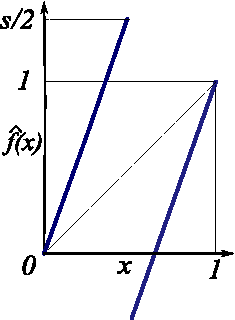
\includegraphics[width=0.36\textwidth]{fig_d_1CL18}
~~~
{(b)}
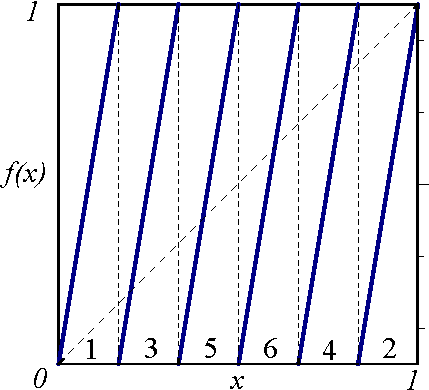
\includegraphics[width=0.32\textwidth]{fig_d_2}
  \caption{\label{fig-d-1}
(a) $\hflow{}{\hx}$, the full space sawtooth map \refeq{KD-map}, $\ExpaEig >
2$.
(b) $\flow{}{x}$, the sawtooth map restricted to the unit circle
\refeq{circ-m}, $\ExpaEig=6$.
            }
\end{figure}
%%%%%%%%%%%%%%%%%%%%%%%%%%%%%%%%%%%%%%%%%%%%%%%%%%%%%%%%%%%%%%%%%%
%
%%%%%%%%%%%%%%%%%%%%%%%%%%%%%%%%%%%%%%%%%%%%%%%%%%%%%%%
\example{Linear code for a piecewise linear map.}{\label{exam:SawtoothLin}
the piecewise linear map of \reffig{fig-d-1}
        \jumpBack{exam:SawtoothLin}
    } % end \example{exam:SawtoothLin}
%%%%%%%%%%%%%%%%%%%%%%%%%%%%%%%%%%%%%%%%%%%%%%%%%%%%%%%

  % siminos/spatiotemp/chapter/examTentLCod.tex
% $Author: predrag $ $Date: 2018-05-04 12:19:38 -0400 (Fri, 04 May 2018) $
% called by siminos/spatiotemp/chapter/tentMapCode.tex
%\section{Any piecewise linear map has ``linear code''}
%\label{exam:tentMapSymbDyn}

%%%%%%%%%%%%%%%%%%%%%%%%%%%%%%%%%%%%%%%%%%%%%%%%%%%%%%%
\example{Tent map linear code.}{\label{exam:TentLCod}
The simplest example of a piece-wise linear unimodal map with a binary (in
general, pruned) symbolic dynamics is the {\em tent map,}
%\reffig{f-log-repeller}\,(a),
\beq
\flow{}{x} =  \left\{ \begin{array}{ll}
f_0(x) = \ExpaEig x       & \mbox{ if } x  < 1/2 \\
f_1(x) =  \ExpaEig (1-x)  & \mbox{ if } x  > 1/2
         \end{array}\right.
\,,
\ee{anyTentSplit}
with $1<\ExpaEig<\infty$ and $x\in\pS=[0,1]$. (Everything would go through for
a skew tent map with $\ExpaEig_0\neq-\ExpaEig_1$, but there is no need here
for that complication.)
For this family of unimodal maps the coarse (covering) partition of the unit
interval $\pS=\pS_0\cap{C}\cap\pS_1$ is given by intervals $\pS_0=[0,1/2)$,
 $\pS_1=(1/2,1]$, and the critical point $C=1/2$.
Let's rewrite this as a linear first-order difference equation, in the manner
of cat lovers enamoured of matters feline:
\beq
\frac{1}{\ExpaEig}  \, x_{t+1}  +(2\Ssym{t}-1)x_{t} = \Ssym{t}
\,,\qquad
\left\{ \begin{array}{ll}
\Ssym{t}=0 & \mbox{ if }  x_{t}  < 1/2 \\
\Ssym{t}=1 & \mbox{ if }  x_{t}  > 1/2
         \end{array}\right.
\,.
\ee{TentLinCode}
That every such code is a `linear code' is best understood by
computing a periodic orbit for a specified itinerary.

The fixed point condition $\flow{n}{x}=x$ for $n$-cycle
\cycle{\Ssym{1}\Ssym{2}\Ssym{3}\cdots \Ssym{n-1}\Ssym{n}}
is a linear relation between the finite alphabet $\Ssym{t}\in\{0,1\}$ code, and
the $x_{t}\in\reals$ orbit
\beq
  \Delta(\Ssym{})q(\Ssym{}) = m(\Ssym{})
\ee{tentMapDiffEq}
with orbit-dependent inverse propagator $\Delta(\Ssym{})= $
\[
{\small
\left(\begin{array}{cccccc}
      {2\Ssym{n}-1}     & 0     &     0  & \dots  & 0 & \ExpaEig^{-1}\\
      \ExpaEig^{-1}     & {2\Ssym{n-1}-1} &     0     &\dots  &  0 & 0\\
       0 & \ExpaEig^{-1} &    {2\Ssym{n-2}-1} &\dots  &  0 & 0\\
      \vdots&\vdots &   \vdots & \ddots &\vdots  &\vdots \\
       0 &  0 &    0  & \dots  & {2\Ssym{2}-1}& 0\\
      0     &  0 &    0  & \dots  &\ExpaEig^{-1}  & {2\Ssym{1}-1}\\
     \end{array} \right)
\,,
} % end \small
\]
\[
q(\Ssym{})= \left(\begin{array}{c}
      x_{{n}}\\
      x_{{n-1}}\\
      x_{{n-2}}\\
      \vdots\\
      x_{{2}}\\
      x_{{1}}\\
     \end{array} \right)
\,,\qquad
m(\Ssym{})= \left(\begin{array}{c}
      {\Ssym{n}}\\
      {\Ssym{n-1}}\\
      {\Ssym{n-2}}\\
      \vdots\\
      {\Ssym{2}}\\
      {\Ssym{1}}\\
     \end{array} \right)
\,,
\]
and $m(\Ssym{})$ is needed to fold the stretched orbit back into the unit
interval.
While the off-diagonal ``1''s do generate cyclic shifts, the diagonal $\pm
\ExpaEig$ terms are not shift invariant, so I do not believe this can be
diagonalized by a discrete Fourier transform. I had worked it out for
$\ExpaEig=2$ in Chaos\-Book, but not sure if there are elegant tricks for
arbitrary $\ExpaEig\neq2$. For an orbit
\beq
  q(\Ssym{}) = \Delta(\Ssym{})^{-1}m(\Ssym{})
\ee{tentMapOrbit}
to be admissible, no point should be to the right of
the kneading value $x_\kappa = f(C)$. It follows from
the kneading theory for unimodal maps (dike map with slope
$\ExpaEig=2$ being the canonical example) that if a \po \ exists for
a given $\ExpaEig$, it exists for all larger $\ExpaEig$,
and that all orbits exist for $\ExpaEig \geq 2$.

In other words, $\ExpaEig$ is the ``stretching parameter'' for this
problem, and the rational polynomial expressions in $\ExpaEig$
for $x_{t}$ correspond to Li Han's polynomials for cat maps.
        \jumpBack{exam:TentLCod}
    } %end \example{Tent map linear code.}{exam:TentLCod}
%%%%%%%%%%%%%%%%%%%%%%%%%%%%%%%%%%%%%%%%%%%%%%%%%%%%%%%%%%%%%%

%%%%%%%%%%%%%%%%%%%%%%%%%%%%%%%%%%%%%%%%%%%%%%%%%%%%%%%%%%%%%%
\example{Periodic points of a tent map.}{\label{exam:TentCycl}

\paragraph{Exercise}
Check \refeq{tentMapOrbit} for fixed point(s).


\paragraph{Exercise}
Check \refeq{tentMapOrbit} for the 2-cycle \cycle{01}.
\[
\Delta(\Ssym{})=
\left(\begin{array}{cc}
      -\ExpaEig& 1\\
      1     & \ExpaEig
     \end{array} \right)
\,,\qquad
m(\Ssym{})= \ExpaEig \left(\begin{array}{c}
      0\\
      1
     \end{array} \right)
\,.
\]
\[
\Delta^{-1} =
\frac{1}{\ExpaEig^2+1}
\left(\begin{array}{cc}
      -\ExpaEig& 1\\
      1     & \ExpaEig
     \end{array} \right)
\,,\qquad
  \det\Delta(\Ssym{})= -(\ExpaEig^2+1)
\]
\[
\left(\begin{array}{c}
      x_{01}\\
      x_{10}
     \end{array} \right)
=
\frac{\ExpaEig}{\ExpaEig^2+1}
\left(\begin{array}{cc}
      -\ExpaEig& 1\\
      1     & \ExpaEig
     \end{array} \right)
\,\left(\begin{array}{c}
      0\\
      1
     \end{array} \right)
=
\frac{\ExpaEig}{\ExpaEig^2+1}
\,\left(\begin{array}{c}
      1\\
      \ExpaEig
     \end{array} \right)
\,.
\]
For the Ulam tent map this
yields the correct periodic points
\(
\{x_{01},x_{10}\}
=\{2/5,4/5\}
\,.
\)
In the $\ExpaEig\to1$ limit, this 2-cycle collapses into the
critical point $C=1/2$.


\paragraph{Exercise}
Check \refeq{tentMapOrbit} for the two 3-cycles.
For the Ulam tent map case, the periodic points are
\bea
\{\gamma_{001},\gamma_{010},\gamma_{100}\}
&=& \{2/9,4/9,8/9\}
\continue
\{\gamma_{011},\gamma_{110},\gamma_{101}\}
&=& \{2/7,4/7,6/7\}
\,.
\nnu
\eea


\paragraph{Exercise}
Check \refeq{tentMapOrbit} for $\ExpaEig =$ golden mean. The $\cycle{001} \to
\cycle{0C1}$ as $\ExpaEig \to $ golden mean from above. Do you get all
admissible cycles? That is worked out in Chaos\-Book, but not in this
formulation.

\paragraph{Exercise}
Is there a systematic solution to \refeq{tentMapOrbit} for arbitrary
$n$-cycle? The $\ExpaEig=2$ case has the elegant solution described in
Chaos\-Book; whatever polynomials you find, they should agree with that
particular factorization. In other words, think of the sums
\refeq{tentEvenCyclePts} and \refeq{tentOddCyclePts} as the expansion of a
real number in terms of the digits $w_t$ in the nonintegral base $\ExpaEig$.
As the symbolic dynamics of a cycle is independent of  $\ExpaEig$, the Ulam
tent map calculation, in the familiar base 2 clinches the arbitrary tent map
case.

\bigskip

    {\color{red}
    The rest of the section might even be right - has to factorize in
    agreement with my Ulam tent map computations. Please fix at your leisure,
    if I am wrong.
    }

\bigskip

If the repeating string                                         \toCB
$\Ssym{1}\Ssym{2}\ldots \Ssym{n}$ contains an even number of
`1's, the repating string of well ordered symbols $w_1w_2\ldots
w_{n}$ is of the same length. The cycle-point $x$ is a geometrical sum which we
can rewrite as the odd-denominator fraction
\bea
   x(\cycle{\Ssym{1}\Ssym{2}\ldots \Ssym{n}})
   &=& \sum_{t=1}^{n} \frac{w_t}{\ExpaEig^{t}}
      +  \frac{1}{\ExpaEig^{-n}} \sum_{t=1}^{n} \frac{w_t}{\ExpaEig^{t}}
      + \cdots
   \continue
   &=& \frac{1}{\ExpaEig^{n}-1}
        \sum_{t=1}^{n} {w_t}{\ExpaEig^{n-t}}
\label{tentEvenCyclePts}
\eea
If the repeating string
$\Ssym{1}\Ssym{2}\ldots \Ssym{n}$ contains an odd number of
`1's, the string of well ordered symbols $w_1w_2\ldots
w_{2n}$ has to be of the double length before it repeats
itself. The cycle-point $x$ is a geometrical sum which we
can rewrite as the odd-denominator fraction
\bea
   x(\cycle{\Ssym{1}\Ssym{2}\ldots \Ssym{n}})
   &=& \sum_{t=1}^{2n} \frac{w_t}{\ExpaEig^{t}}
      +  \frac{1}{\ExpaEig^{-2n}} \sum_{t=1}^{2n} \frac{w_t}{\ExpaEig^{t}}
      + \cdots
   \continue
   &=& \frac{1}{(\ExpaEig^{n}-1)(\ExpaEig^{n}+1)}
        \sum_{t=1}^{2n}{w_t}{\ExpaEig^{2n-t}}
\label{tentOddCyclePts}
\eea
        \jumpBack{exam:TentCycl}
    } %end \example{Tent map linear code.}{exam:TentCycl}
%%%%%%%%%%%%%%%%%%%%%%%%%%%%%%%%%%%%%%%%%%%%%%%%%%%%%%%%%%%%%%

  % siminos/spatiotemp/chapter/examBelykhLCod.tex
% $Author: predrag $ $Date: 2021-12-24 01:25:20 -0500 (Fri, 24 Dec 2021) $

% siminos/spatiotemp/chapter/examTentLCod.tex
% $Author: predrag $ $Date: 2021-12-24 01:25:20 -0500 (Fri, 24 Dec 2021) $
% called by siminos/spatiotemp/chapter/tentMapCode.tex
%\section{Any piecewise linear map has ``linear code''}
%\label{exam:tentMapSymbDyn}

%%%%%%%%%%%%%%%%%%%%%%%%%%%%%%%%%%%%%%%%%%%%%%%%%%%%%%%
\example{Belykh map linear code.}{\label{exam:BelykhLCod}
Li and Xie\rf{LiXie16}
{\em Symbolic dynamics of {Belykh}-type maps}:
``
The symbolic dynamics of a Belykh-type map (a two-dimensional
discontinuous piecewise linear map) is investigated. The pruning front
conjecture (the admissibility condition for symbol sequences)  is proved
under a hyperbolicity condition. Using this result, a symbolic dynamics
model of the map is constructed according to its pruning front and
primary pruned region.
''

The Belykh map is a piecewise linear map given by
\[  \left( \begin{array}{c}
        x_{n+1} \\
        y_{n+1} \\
        \end{array}\right)
        = \left(\begin{array}{c}
                    \sign{n} -a x_n + b y_n     \\
                    x_n                         \\
                \end{array} \right)
        =  \left( \begin{array}{c}
            \sign{n} \\
            0        \\
        \end{array}\right)
        +
\left(\begin{array}{cc}
            -a  & b      \\
             1  & 0      \\
                \end{array} \right)
\left( \begin{array}{c}
        x_{n} \\
        y_{n} \\
        \end{array}\right)
\,.\]
where
\[
\sign{n} = \left\{\begin{array}{rcc}
                                1 & \mbox { if } &  x_n \geq 0\\
                                -1 & \mbox { if } &  x_n < 0\\
                                                \end{array} \right.
\,.
\]
The two branches of the map are
\[
f_{\pm} = \left\{\begin{array}{l}
                                \pm 1 -a x + b y\\
                                 x \\
                                                \end{array} \right.
\,.\]
In the 3-term recurrence formulation (the linear code), the map is
an asymmetric tridiagonal Toeplitz matrix
\[
 x_{n+1} +a x_n - b x_{n-1} = \sign{n}
 \,,
\]
or
\beq
\Box x_n +(2+a) x_n - (1+b) x_{n-1} = \sign{n}
 \,.
\ee{s:BelykhMapDiff}
For $b=-1$ (the Hamiltonian, time-reversible case) this is almost the cat
map, with $a=-s$, except that the single sawtooth discontinuity is across
$x=0$, there is no $\mod\ 1$ condition.

Li and Xie consider the
\(
a,\, b\, > 0
\)
case. The strange attractor (for example, for $a = 1.5$ and $b = 0.3$)
looks like a fractal set of parallel lines.
They define the pruning front, the primary pruned region, plot them in
the symbol plane, and prove the pruning front conjecture  for this map.
In the symbol plane there is a symmetry under rotation by $\pi$, but they
do not seem to exploit that.

They call the past and the future itineraries of the tail and the head,
and start the head with $s_0$.

T{\'{e}}l\rf{Tel83} {\em Fractal dimension of the strange attractor in a
piecewise linear two-dim\-en\-si\-on\-al map} computes the box-counting dimension
of this map (which he does not call Belykh map).
    } % end \example{Belykh map linear code.}{{exam:BelykhLCod}

  % siminos/spatiotemp/chapter/examLoziLCod.tex
% $Author: predrag $ $Date: 2021-12-24 01:25:20 -0500 (Fri, 24 Dec 2021) $


%%% input by % siminos/spatiotemp/chapter/catMap.tex %%%%%
%\section{Any piecewise linear map has ``linear code''}
%\label{exam:tentMapSymbDyn}

%%%%%%%%%%%%%%%%%%%%%%%%%%%%%%%%%%%%%%%%%%%%%%%%%%%%%%%
\example{Lozi map linear code.}{\label{exam:LoziLCod}
The Lozi map
\[
    x_{n+1}=1- \sign{n} ax_{n} +bx_{n-1} \, .
\]
written as a 3-term recurrence relation
\beq
    x_{n+1}-2x_{n}+x_{n-1}+(2+\sign{n} a)x_{n} -(b+1)x_{n-1}=1
\, .
\ee{Lozi2-step}
That has the same nonlinear term $\sign{n} x_{n}$ as \refeq{TentLinCode},
so maybe we can figure out the pruning front as well, in this
formulation.
        \jumpBack{exam:LoziLCod}
    } % end \example{Lozi map linear code.}{exam:TentCycl}
%%%%%%%%%%%%%%%%%%%%%%%%%%%%%%%%%%%%%%%%%%%%%%%%%%%%%%%

%\newpage
  \Problems{exerCatMap}{7mar2018}
% siminos/spatiotemp/Problems/exerCatMap.tex called by catMap.tex
% $Author: predrag $ $Date: 2021-06-12 01:01:43 -0400 (Sat, 12 Jun 2021) $

% Predrag                                               23jan2018

%%%%%%%%%%%%%%%%%%%%%%%%%%%%%%%%%%%%%%%%%%%%%%%%%%%%%%%%%%%%%%%%%%%
\exercise{Cat map Green's function, infinite lattice.}{\label{exer:catMapGreenInf}

(a) Show that the eigenvalues of the cat map $M$ are
given by
\beq
\ExpaEig^{\pm}=\frac{1}{2}(s\pm \surd{D})
\,,\qquad
\ExpaEig=e^{\Lyap}
\,,
\ee{catEigsEx}
where $\ExpaEig\equiv\ExpaEig^+$, $s=\ExpaEig+\ExpaEig^{-1}$,
$\surd{D}=\ExpaEig-\ExpaEig^{-1}$, and the discriminant is $D={s^{2}-4}$.

(b) Verify by substitution that the Green's function is given by
\beq
\gd_{nn'}= \frac{1}{{\surd{D}}}\,\frac{1}{\ExpaEig^{|n'-n|}}
\,.
\ee{GreenFun00b}

(c) Show that the orbit is then recovered by
\beq
\ssp_{n} =  \frac{1}{{\surd{D}}}
\sum_{n' \in \integers} \ExpaEig^{- |n-n'|} \Ssym{n'}
\,.
\label{BirVivx=s}
\eeq
    } % end \exercise{exer:catMapGreenInf}
%%%%%%%%%%%%%%%%%%%%%%%%%%%%%%%%%%%%%%%%%%%%%%%%%%%%%%%%%%%%%%%%%%%%%%%%

%%%%%%%%%%%%%%%%%%%%%%%%%%%%%%%%%%%%%%%%%%%%%%%%%%%%%%%%%%%%%%%%%%%
\exercise{Cat map Green's function for a \po.}{\label{exer:catMapGreenPBC}
Show that the Green's function for a \po\ of period $\cl{p}$ is
obtained by summing \refeq{GreenFun00b} over period \cl{p}:
\beq
g^p_{nn'}=\sum_{j=-\infty}^{\infty}{g}_{n-n',j\cl{p}}
  =\frac{1}{{\surd{D}}}\,\frac{\ExpaEig^{-|n-n'|}+\ExpaEig^{-\cl{p}+|n-n'|}}
        {1-\ExpaEig^{-\cl{p}}}
\,.
\ee{GreenFun2}
Verify this formula by explicit matrix inversion for a few periodic points
of cycles $p$ of
periods $\cl{p}=1,2,3,4,\cdots$.
    } % end \exercise{exer:catMapGreenPBC}
%%%%%%%%%%%%%%%%%%%%%%%%%%%%%%%%%%%%%%%%%%%%%%%%%%%%%%%%%%%%%%%%%%%%%%%%

%%%%%%%%%%%%%%%%%%%%%%%%%%%%%%%%%%%%%%%%%%%%%%%%%%%%%%%%%%%%%%%%%%%
\exercise{$d=2$ cat map guess Green's function, infinite lattice.}{\label{exer:catMapGreend=2wrong}
% Predrag 2018-03-11 wrong guess, debunked by Han
Show by substitution that a $d=2$ ``Green's function'' guess given by
\beq
\gd_{z z'}= \PCedit{\frac{1}{2}}\frac{1}
            {{\surd{D}}}\,\frac{1}{\ExpaEig^{|\ell'-\ell|+|t'-t|}}
\,,
\ee{GreenFund=2wrong}
(and similarly, in arbitrary dimension $d>1$) \emph{does not} satisfy the
Green's function conditions
\beq
(\D \gd)_{zz'}=\delta_{zz'}=\delta_{ll'}\delta_{tt'}
\,,
\ee{HLGreenFund=2C}
Here the eigenvalues of the cat map $M$ are
\beq
\ExpaEig^{\pm}=\frac{1}{2}(s/2 \pm \surd{D})
\,,\qquad
\ExpaEig=e^{\Lyap}
\,,
\ee{catEigsEx2D}
where $\ExpaEig\equiv\ExpaEig^+$, $s/2=\ExpaEig+\ExpaEig^{-1}$,
$\surd{D}=\ExpaEig-\ExpaEig^{-1}$, and the discriminant is $D={(s/2)^{2}-4}$.

Hint: the check works just like for \refexer{exer:catMapGreenInf}.
    } % end \exercise{exer:catMapGreend=2wrong}
%%%%%%%%%%%%%%%%%%%%%%%%%%%%%%%%%%%%%%%%%%%%%%%%%%%%%%%%%%%%%%%%%%%%%%%%

%%%%%%%%%%%%%%%%%%%%%%%%%%%%%%%%%%%%%%%%%%%%%%%%%%%%%%%%%%%%%%%%%%%
\exercise{\Po s of Arnol'd cat map.}{\label{exer:AKScatMapPOs}
% moved to here from {blogAKS}{2016-06-09}
\begin{enumerate}
  \item %[[X]]
Describe precisely how you actually pick ``random $q_1$ and $q_2$''
  \item %[[X]]
Explain what happens if $q_1$ and $q_2$ are rational
  \item %[[X]]
Can you get a \po\ if $q_1$ and $q_2$ are irrational?
  \item %[[X]]
What do you mean by period $0$?
  \item %[[X]]
Does the Arnol'd cat map have \po s of any period?
  \item %[[X]]
Derive analytically that $m_j \in \{-1, 0,  1,2\}$ (you can continue the
exposition that I started in \refsect{sect:PerViv}, if that helps). Does you
result agree with Percival and Vivaldi\rf{PerViv}?
\end{enumerate}
%                                       \PCpost{2016-06-02}{:
}
%%%%%%%%%%%%%%%%%%%%%%%%%%%%%%%%%%%%%%%%%%%%%%%%%%%%%%%%%%%%%%%%%%%%

%%%%%%%%%%%%%%%%%%%%%%%%%%%%%%%%%%%%%%%%%%%%%%%%%%%%%%%%%%%%%%%%%%%
\exercise{The second iterate generating partition.}{\label{exer:n=2GenPart}
%    \PCpost{2019-08-10}{
\refFig{fig:PVAdlerWeissS} is very helpful in giving us a visual
understanding of what a Hamiltonian cat map does, and how the generating
partition comes about. Draw the corresponding \AW\ generating partition
for $s=3$, the second, $n=2$ iterate, to verify that the $n=1$ determines
a generating partition for all subsequent times.
    } % end \exercise{exer:n=2GenPart}
%%%%%%%%%%%%%%%%%%%%%%%%%%%%%%%%%%%%%%%%%%%%%%%%%%%%%%%%%%%%%%%%%%%%%%%%

%%%%%%%%%%%%%%%%%%%%%%%%%%%%%%%%%%%%%%%%%%%%%%%%%%%%%%%%%%%%%%%%%%%
%\exercise{XXX.}{\label{exer:XXX}
%XXX
%    } % end \exercise{exer:XXX}
%%%%%%%%%%%%%%%%%%%%%%%%%%%%%%%%%%%%%%%%%%%%%%%%%%%%%%%%%%%%%%%%%%%%%%%%

%%%%%%%%%%%%%%%%%%%%%%%%%%%%%%%%%%%%%%%%%%%%%%%%%%%%%%%%%%%%%%%%%%%
%\exercise{XXX.}{\label{exer:XXX}
%XXX
%    } % end \exercise{exer:XXX}
%%%%%%%%%%%%%%%%%%%%%%%%%%%%%%%%%%%%%%%%%%%%%%%%%%%%%%%%%%%%%%%%%%%%%%%%

    \ProblemsEnd

  \Solution{catMap}{soluCatMap}{23jan2018}{Cat map}
% siminos/spatiotemp/Solutions/soluCatMap.tex called by catMap.tex
% $Author: predrag $ $Date: 2021-08-10 11:56:19 -0400 (Tue, 10 Aug 2021) $

% Predrag                                               23jan2018

%%%%%%%%%%%%%%%%%%%%%%%%%%%%%%%%%%%%%%%%%%%%%%%%%%%%%%%%%%%%%%%%%%%
\solution{exer:catMapGreenInf}{Cat map Green's function, infinite lattice.}{

(a) It's just the roots of a quadratic equation, with
\(
s=\ExpaEig+\ExpaEig^{-1}
\,,
\)
and \(
\surd{D}=\ExpaEig-\ExpaEig^{-1}
\,.
\)


(b) The Green's function \refeq{GreenFun00b}
\beq
\gd_{tt'}=  \frac{1}{{\surd{D}}}\,\frac{1}{\ExpaEig^{|t'-t|}}
\ee{GreenFun00d}
for the discrete damped Poison
equation \refeq{eq:CatMapStep} was first computed explicitly by Percival and
Vivaldi\rf{PerViv}, using the methods introduced in Mestel and
Percival\rf{varcyc}. It should satisfy
\beq
(\D \gd)_{ij} = \sum_{k} \D_{ik} \gd_{kj} =\delta_{ij}
\,.
\ee{HLGFuncInf1}
Since we are considering infinite $1D$ lattice, we do not need to
specify the boundary conditions. $\D$ is a Toeplitz matrix
\beq
\D_{ik}=s \delta_{ik} - \delta_{i-1,k} - \delta_{i+1,k}
\ee{HLGFuncInf2}
Substituting \refeq{HLGFuncInf2} into \refeq{HLGFuncInf1}
\beq
\sum_{k} \D_{ik} \gd_{kj} = s \gd_{ij} -\gd_{i-1,j}-\gd_{i+1,j} =\delta_{ij}
\,,
\ee{HLGFuncInf3}
and substituting \refeq{GreenFun00b}
\beq
\gd_{ij}= \frac{1}{\surd{D}}\,
          \frac{1}{\ExpaEig^{|j-i|}}
=  \left\{ \begin{array}{ll}
\frac{1}{\surd{D}}\,\frac{1}{\ExpaEig^{i-j}}  & \mbox{ if } j < i  \\
\frac{1}{\surd{D}} & \mbox{ if } j = i  \\
\frac{1}{\surd{D}}\,\frac{1}{\ExpaEig^{j-i}}  & \mbox{ if } j > i
         \end{array}\right.
\,.
\ee{GreenFun00c}
into \refeq{HLGFuncInf3},
one verifies that \refeq{GreenFun00b} is indeed the Green's function
for the infinite lattice. By translational invariance, for $i=j$ consider
\beq
s \gd_{00} -\gd_{-1,0}-\gd_{10}
  = \frac{1}{\surd{D}}\,\left(
  {s} - \frac{2}{\ExpaEig}
     \right)
  = \frac{1}{\surd{D}}\,\left(\ExpaEig-\frac{1}{\ExpaEig}\right)
  = 1
\,.
\label{HLGFuncInf5}
\eeq
For $i>j$ consider
\beq
s \gd_{10} -\gd_{00}-\gd_{20}
  = \frac{1}{\surd{D}}\,\left(
  \frac{s}{\ExpaEig}
  - 1
  - \frac{1}{\ExpaEig^{2}}
     \right)
  = \frac{1}{\surd{D}}\,\frac{1}{\ExpaEig}
      \,\left( s - \ExpaEig-\frac{1}{\ExpaEig}\right)
  = 0
\,.
\label{HLGFuncInf4}
\eeq

(c) The orbit is recovered by:
\beq
\ssp_n=\sum_{n' \in \integers} \gd_{nn'} \Ssym{n'}
= \frac{1}{{\surd{D}}} \sum_{n' \in \integers} \ExpaEig^{- |n-n'|} \Ssym{n'}
\,.
\ee{HLGFuncInf6}
\hfill (Han Liang) %{2018-03-08}{
    } % end \solution{exer:catMapGreenInf}
%%%%%%%%%%%%%%%%%%%%%%%%%%%%%%%%%%%%%%%%%%%%%%%%%%%%%%%%%%%%%%%%%%%%%%%%

%%%%%%%%%%%%%%%%%%%%%%%%%%%%%%%%%%%%%%%%%%%%%%%%%%%%%%%%%%%%%%%%%%%
\solution{exer:catMapGreenPBC}{Cat map Green's function for a \po.}{
%    \PC{2017-08-28} {
%``Average coordinate'' depends on b.c.'s. Average coordinate
%\refeq{catMapAverCoord} is computed for
%the the very unphysical Dirichlet boundary condition $\ssp_z=0$ for $z\in \R$
%which breaks translation invariance.
%If one takes the much gentler, translationally invariant doubly periodic b.c.,
%the ``average coordinate'' $\bar{x}_z$ is the \twot\ periodic point, a
%more natural choice.
%    }
Express the periodic orbit Green's function in terms of the infinite
lattice by using a periodic source $\Ssym{n'}=\Ssym{n'}+\cl{p}$,
\bea
\sum_{n'=-\infty}^{\infty}\gd_{nn'}\Ssym{n'}
 &=& \sum_{r=-\infty}^{\infty} \sum_{n'=r\cl{p}}^{r\cl{p}+\cl{p}-1}\gd_{nn'}\,\Ssym{n'}
= \sum_{r=-\infty}^{\infty} \sum_{n'=0}^{\cl{p}-1}\gd_{n,n'+r\cl{p}}\,\Ssym{n'+r\cl{p}}
\continue
 &=& \sum_{r=-\infty}^{\infty} \sum_{n'=0}^{\cl{p}-1}\gd_{n-n',r\cl{p}}\,\Ssym{n'}
\label{HLGFuncPO1}
\eea
Comparing with the expression for the Green's function of a periodic orbit:
\beq
\sum_{n'=0}^{\cl{p}-1}\gd_{nn'}^\cl{p} \Ssym{n'}
\label{HLGFuncPO2}
\eeq
we see that
\beq
\gd_{nn'}^\cl{p}=\sum_{r=-\infty}^{\infty} \gd_{n-n',r\cl{p}}
\ee{HLGFuncPO3}
Substituting \refeq{GreenFun00b} into \refeq{HLGFuncPO3} we have:
%\beq
%	\gd_{n,n'}^P
%	&=& \frac{1}{\surd{D}}\sum_{r=-\infty}^{\infty} \frac{1}{\ExpaEig^{|n-n'-rP|}}
%\ee{HLGFuncPO4}
% HL could not print this. PC should have used \bea ... \label{HLGFuncPO4}\eea
\bea
   \gd_{nn'}^\cl{p}
   &=& \frac{1}{\surd{D}}\sum_{r=-\infty}^{\infty} \frac{1}{\ExpaEig^{|n-n'-r\cl{p}|}}
   \continue
   &=& \frac{1}{\surd{D}} \left( \frac{1}{\ExpaEig^{|n-n'|}}
   +\sum_{r=1}^{\infty} \frac{1}{\ExpaEig^{r\cl{p}-(n-n')}}
   + \sum_{r=-1}^{-\infty} \frac{1}{\ExpaEig^{(n-n')-r\cl{p}}}
   \right)
   \continue
   &=& \frac{1}{\surd{D}} \left(  \frac{1}{\ExpaEig^{|n-n'|}}
   +\frac{1}{\ExpaEig^{-|n-n'|}}\frac{1}{\ExpaEig^\cl{p}-1}
   +\frac{1}{\ExpaEig^{|n-n'|}}\frac{1}{\ExpaEig^\cl{p}-1}
   \right)
   \continue
   &=& \frac{1}{\surd{D}}\,
       \frac{1}{1-\ExpaEig^{-\cl{p}}}
       (\ExpaEig^{-|n-n'|} + \ExpaEig^{-\cl{p}+|n-n'|})
   \label{HLGFuncPO4}
\eea
This verifies \refeq{GreenFun2}.

Bird and Vivaldi\rf{BirViv} show that for an $n$-cycle $\ssp_{n'}$ are
rational functions of $\ExpaEig$, given by the quotient of two reflexive
polynomials
(for example, $P_t(\ExpaEig)= \ExpaEig^n P_t(1/\ExpaEig)$),
\bea
\ssp_{t} &=&  \ExpaEig \,{P_t(\ExpaEig)}/{Q(\ExpaEig)}
        \continue
P_t(\ExpaEig) &=&  \sum_{\tau=1}^{n-1}
                   \ExpaEig^{n-\tau}(\ExpaEig\,\Ssym{t+\tau-1} + \Ssym{t-\tau})
        \continue
Q(\ExpaEig) &=&  (\ExpaEig^2 - 1)\,(\ExpaEig^n - 1)
\label{BirViv(3.5)a}
\eea
Bird and Vivaldi\rf{BirViv} then discuss pruning, give formulas for the
numbers of {\orbit}s for integer $s$, \etc.

\hfill (Han Liang) %{2018-03-08}
    } % end \solution{exer:catMapGreenPBC}
%%%%%%%%%%%%%%%%%%%%%%%%%%%%%%%%%%%%%%%%%%%%%%%%%%%%%%%%%%%%%%%%%%%%%%%%

%%%%%%%%%%%%%%%%%%%%%%%%%%%%%%%%%%%%%%%%%%%%%%%%%%%%%%%%%%%%%%%%%%%
\solution{exer:catMapGreend=2wrong}{$d=2$ cat map guess Green's function, infinite lattice.}{
% \HLpost{2018-03-12}{ The Green's function \refeq{GreenFund=2wrong} is not correct.
The Green's function $\gd$ for the Toeplitz matrix (tensor) in 2 dimensions
\bea
\D_{lt,l't'} &=& \left[-\Box + 2\left({s}/{2} - 2\right)\right]_{lt,l't'}
\continue
&=& \left(\frac{s}{2}\delta_{ll'}-\delta_{l-1,l'}-\delta_{l+1,l'}\right)\delta_{tt'}
\ceq
   +\delta_{ll'}\left(\frac{s}{2}\,\delta_{tt'}-\delta_{t-1,t'}-\delta_{t+1,t'}\right)
\,.
\label{HLGreenFund=2B}
\eea
should satisfy \refeq{HLGreenFund=2C},
or, substituting \refeq{HLGreenFund=2B} into \refeq{HLGreenFund=2C},
\bea
\PCedit{2\,}
\delta_{ll'}\delta_{tt'}
   &=& \frac{s}{2}\gd_{ll',tt'}-\gd_{l-1,l',tt'}-\gd_{l+1,l',tt'}
\ceq
     + \frac{s}{2}\gd_{ll',tt'}-\gd_{ll',t-1,t'}-\gd_{ll',t+1,t'}
\,.
\label{HLGreenFund=2D}
\eea
Let's check this.
By translational invariance, need to look only at different values of
$l-l'$ and $t-t'=0$. For $l=l'$ and $t=t'$ it suffices that we consider
the $l=l'=t=t'=0$ case. Using \refeq{catEigsEx2D} we have
\bea
&&\frac{s}{2} \gd_{00,00} -\gd_{-1,0,00}-\gd_{10,00}
\ceq
+ \frac{s}{2} \gd_{00,00} -\gd_{00,-1,0}-\gd_{00,10}
\ceq
  = \frac{2}{\surd{D}}\,\left(
    \frac{s}{2} - \frac{2}{\ExpaEig}
     \right)
  = \frac{2}{\surd{D}}\,\left(\ExpaEig-\frac{1}{\ExpaEig}\right)
  = 2
\,,
\label{HLGFuncInf5a}
\eea
verifies \refeq{HLGreenFund=2B}.

For $l>l'$ and $t=t'$ it suffices
to consider $l=1,l'=0$, $t=t'=0$  case.
\bea
&&\frac{s}{2} \gd_{10,00} -\gd_{00,00}-\gd_{20,00}
    \ceq
 + \frac{s}{2} \gd_{10,00} -\gd_{10,-1,0}-\gd_{10,10}
\ceq
  = \frac{1}{2\surd{D}}\,\left(
  \frac{s/2}{\ExpaEig}
  - 1
  - \frac{1}{\ExpaEig^{2}}
     \right)
  + \frac{1}{2\surd{D}}\,\left(
  \frac{s/2}{\ExpaEig}
   - \frac{2}{\ExpaEig^{2}}
     \right)
\ceq
  = \frac{1}{2\ExpaEig\surd{D}}\,\left(
        \frac{s}{2} - \frac{2}{\ExpaEig^{}}
     \right)
  = \frac{1}{2\ExpaEig\surd{D}}
      \,\left(\ExpaEig-\frac{1}{\ExpaEig}\right)
  = \frac{1}{2\ExpaEig}
\,.
\label{HLGFuncInf4b}
\eea
%\PCedit{2017-03-15 Han is right,
So, the guess \refeq{GreenFund=2wrong} already does not work.

Substitute \refeq{GreenFund=2wrong} into \refeq{HLGreenFund=2D} we get:
\bea
\sum_{z''}\D_{zz''}\gd_{z''z'}
=  \left\{ \begin{array}{ll}
\frac{1}{\surd{D}}\,\frac{1}{\ExpaEig^{|\ell'-\ell|+|t'-t|}} (s-2\ExpaEig-2\ExpaEig^{-1})
           & \mbox{ if } l\neq l'\,and\,t\neq t'   \\
\frac{1}{\surd{D}} (s-4\ExpaEig^{-1})
           & \mbox{ if } l=l'\, and\, t=t'
         \end{array}\right.
\,.
\label{HLGreenFund=2E}
\eea

To satisfy \refeq{HLGreenFund=2C}, $s$, $\surd{D}$ and $\ExpaEig$ must satisfy:
\bea
\left\{ \begin{array}{ll}
s=2\ExpaEig+2\ExpaEig^{-1} \\
\surd{D} = 2\ExpaEig-2\ExpaEig^{-1}
         \end{array}\right.
\,.
\label{HLGreenFund=2F}
\eea
So we will have:
\bea
\left\{ \begin{array}{ll}
\ExpaEig = \frac{1}{4}(s+\sqrt{s^2-16})\\
\ExpaEig^{-1} = \frac{1}{4}(s-\sqrt{s^2-16})
         \end{array}\right.
\,.
\label{HLGreenFund=2G}
\eea
Now the problem is, if $l \neq l'$ but $t = t'$, \refeq{HLGreenFund=2E} become:
\beq
\sum_{z''}\D_{zz''}\gd_{z''z'}
  = \frac{1}{\surd{D}}\,\frac{1}{\ExpaEig^{|\ell'-\ell|+|t'-t|}} (s-\ExpaEig-3\ExpaEig^{-1})
\ee{HLGreenFund=2H}
and this is not satisfied by \refeq{HLGreenFund=2G}. So
\refeq{GreenFund=2wrong} does not work for the 2-dimensional case. I
haven't figured out the correct Green's function for the 2 dimensions.

\hfill (Han Liang) %{2018-03-12}
    } % end \solution{exer:catMapGreend=2wrong}
%%%%%%%%%%%%%%%%%%%%%%%%%%%%%%%%%%%%%%%%%%%%%%%%%%%%%%%%%%%%%%%%%%%%%%%%

%%%%%%%%%%%%%%%%%%%%%%%%%%%%%%%%%%%%%%%%%%%%%%%%%%%%%%%%%%%%%%%%%%%
\solution{exer:catMapGreend=2wrong}{$d=2$ cat map guess Green's function, infinite lattice.}{
%\HLpost{2018-03-15}{
The guess Green's function \refeq{GreenFund=2wrong} doesn't work.
For $l=2$, $l'=0$ and $t=t'=0$, the correct form of \refeq{HLGFuncInf4b} is:
\bea
&&\frac{s}{2} \gd_{10,00} -\gd_{00,00}-\gd_{20,00}
\ceq
+ \frac{s}{2} \gd_{10,00} -\gd_{10,10}-\gd_{10,-10}
\\
  &=& \frac{1}{2\surd{D}}\,\left(
  \frac{s}{2\ExpaEig}
  - 1
  - \frac{1}{\ExpaEig^{2}}
     \right)+
     \frac{1}{2\surd{D}}\,\left(
  \frac{s}{2\ExpaEig}
  - \frac{1}{\ExpaEig^{2}}
  - \frac{1}{\ExpaEig^{2}}
     \right)
   \\
  &=& \frac{1}{2\surd{D}}\,\frac{1}{\ExpaEig}
      \,\left( \frac{s}{2} - \ExpaEig-\frac{1}{\ExpaEig}\right)
      +\frac{1}{2\surd{D}}\,\frac{1}{\ExpaEig}\,\left(
  \frac{s}{2}
  - \frac{1}{\ExpaEig}
  - \frac{1}{\ExpaEig}
     \right)\\
  &=& 0 + \frac{1}{2\ExpaEig}
\,.
\label{HLGFuncInf4I}
\eea
%\PCedit{2017-03-15
As in \refeq{HLGFuncInf4b}, this does not work .

\hfill (Han Liang) %{2018-03-12}
    } % end \solution{exer:catMapGreend=2wrong}
%%%%%%%%%%%%%%%%%%%%%%%%%%%%%%%%%%%%%%%%%%%%%%%%%%%%%%%%%%%%%%%%%%%%%%%%


%%%%%%%%%%%%%%%%%%%%%%%%%%%%%%%%%%%%%%%%%%%%%%%%%%%%%%%%%%%%%%%%%%%
\solution{exer:AKScatMapPOs}{\Po s of Arnol'd cat map.}{
No solution available.
} % end \solution{e-trajectNotIntersect}
%%%%%%%%%%%%%%%%%%%%%%%%%%%%%%%%%%%%%%%%%%%%%%%%%%%%%%%%%%%%%%%%%%%

%%%%%%%%%%%%%%%%%%%%%%%%%%%%%%%%%%%%%%%%%%%%%%%%%%%%%%%%%%%%%%%%%%%
\solution{exer:n=2GenPart}{The second iterate generating partition.}{
%	\HLpost{2019-08-10}{
\refFig{fig:PVAdlerWeiss2Steps} is the generating partition with $s=3$
evolved after 2 steps. In the Markov diagram
\reffig{fig:PVAdlerWeiss2Steps}\,(d) there are 7 self cycles, two of which
are the over-counted fixed points at the origin. So there are actually 5
periodic points with period 2, including 1 fixed point and 2 length-2
{\orbit}s, as given by \refeq{noPrimeCycs=3}.

%%%%%%%%%%%%%%%%%%%%%%%%%%%%%%%%%%%%%%%%%%%%%%%%%%%%%%%%%%%%
	\begin{figure}\begin{center}
            \begin{minipage}[c]{0.36\textwidth}\begin{center}
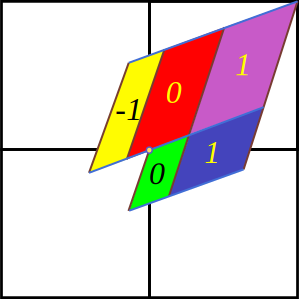
\includegraphics[width=1.0\textwidth]{PVAdlerWeissB-c}\\(a) %{PVAdlerWeiss2Steps-a}\\(a)
\\
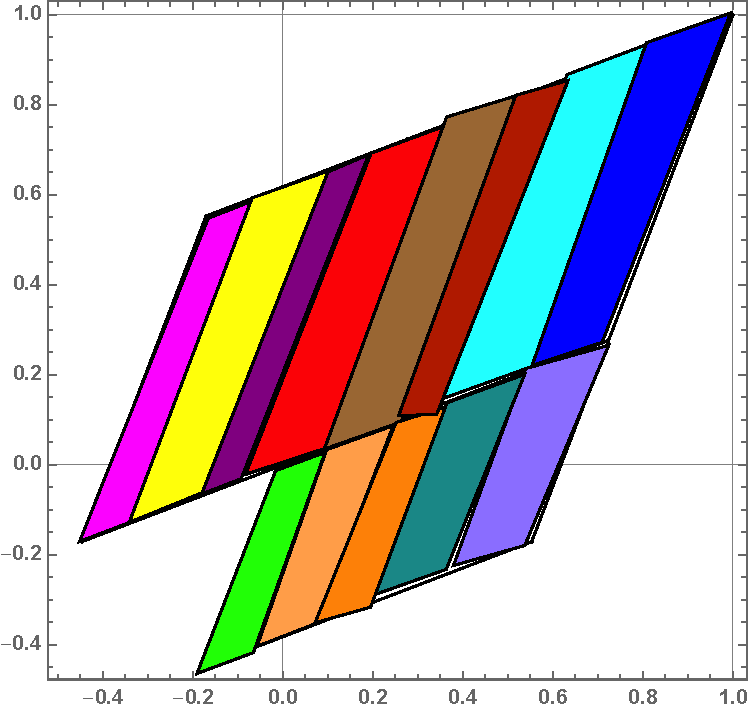
\includegraphics[width=1.0\textwidth]{PVAdlerWeiss2Steps-c}\\(c)
            \end{center}\end{minipage}
            \begin{minipage}[c]{0.3\textwidth}\begin{center}
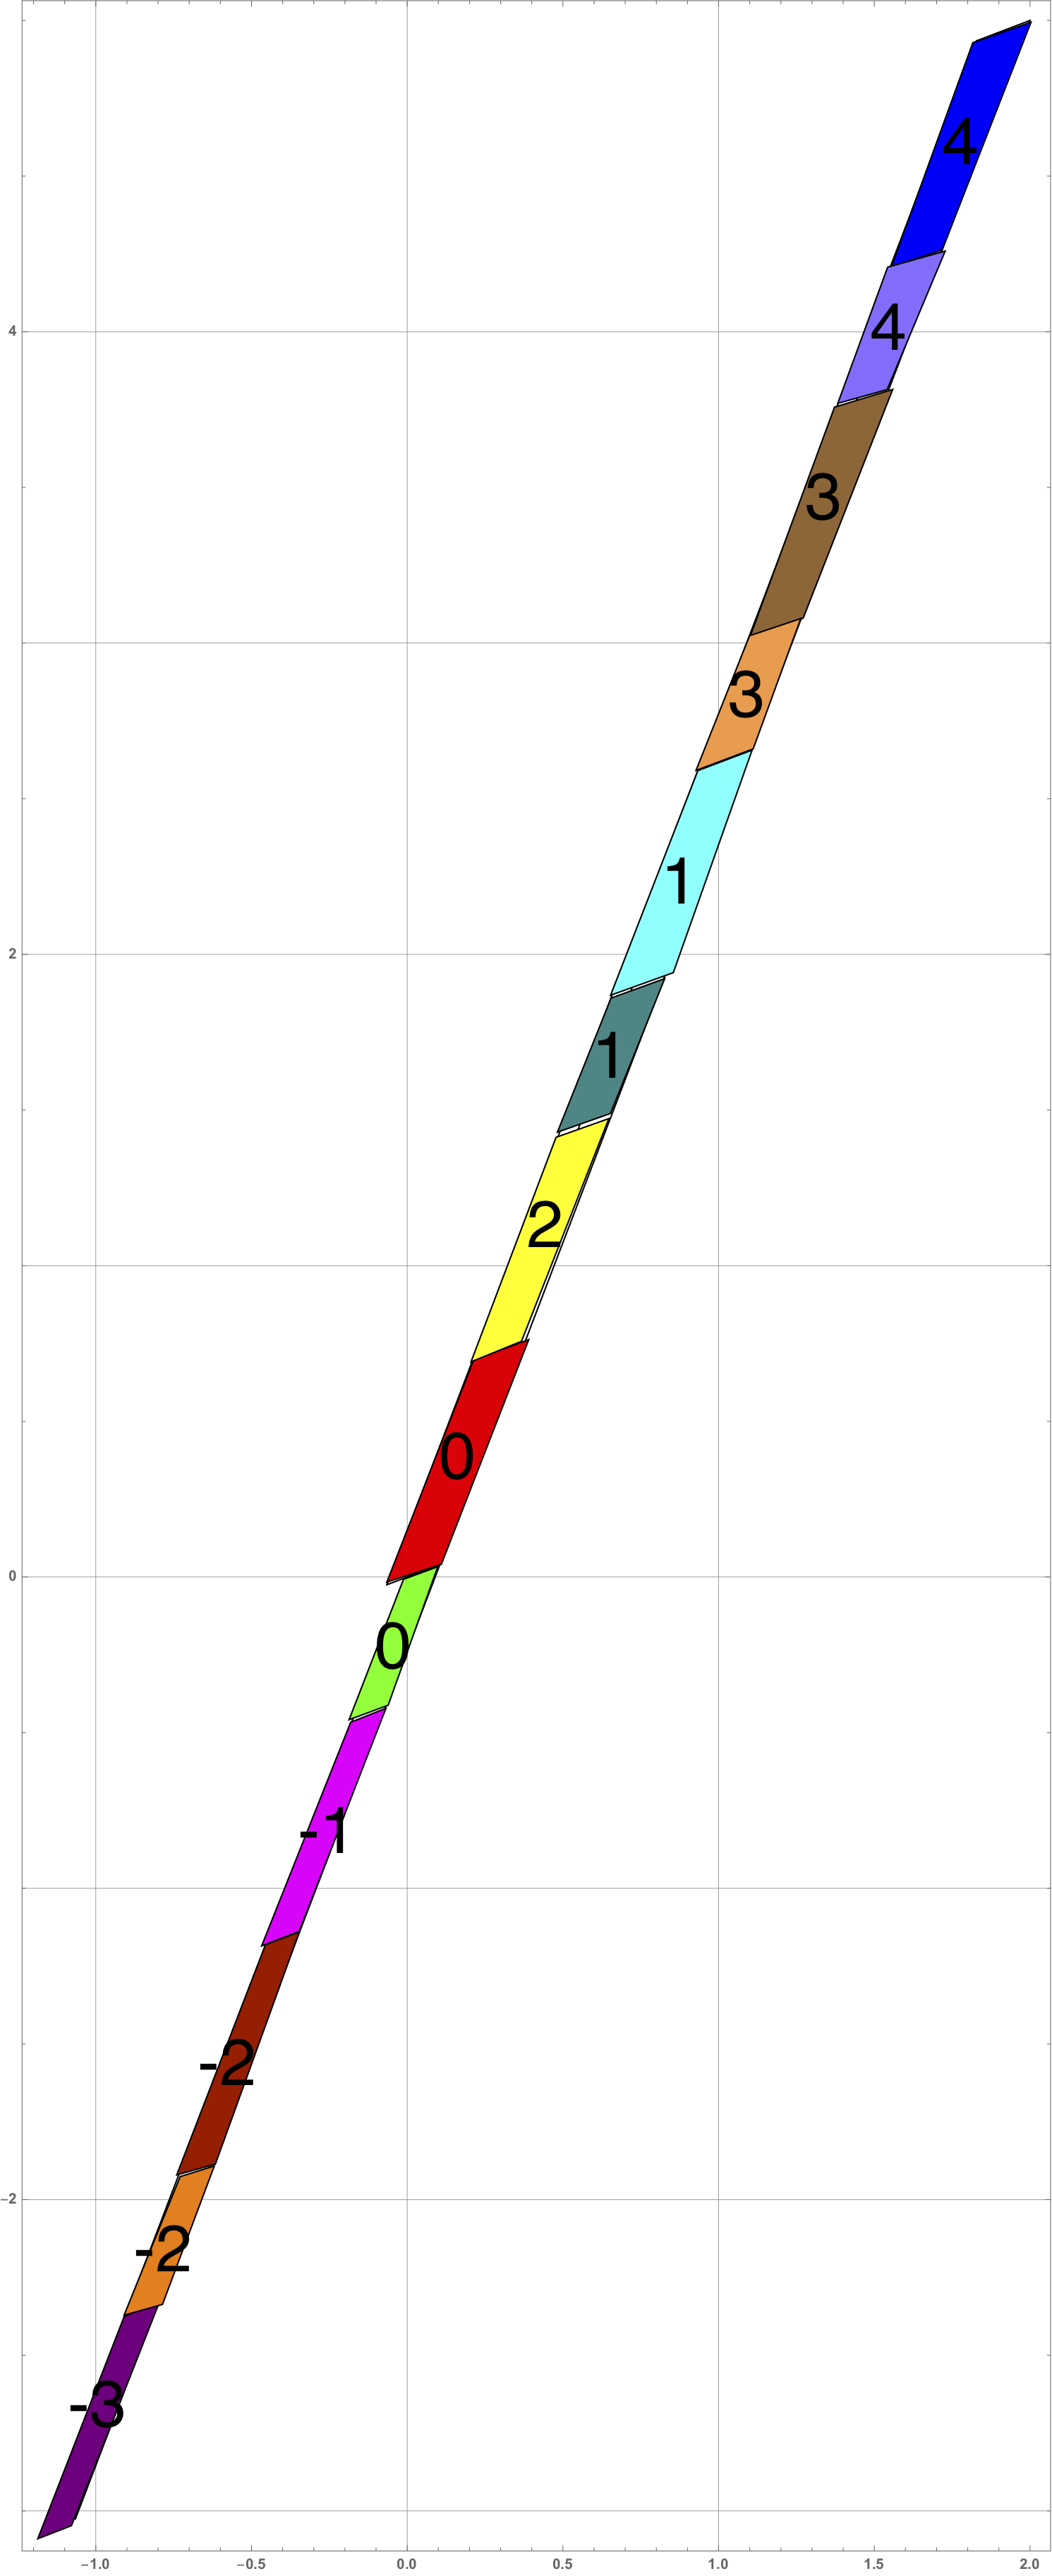
\includegraphics[width=1.0\textwidth]{PVAdlerWeiss2Steps-b}\\(b)
            \end{center}\end{minipage}
            ~~~
            \begin{minipage}[c]{0.25\textwidth}\begin{center}
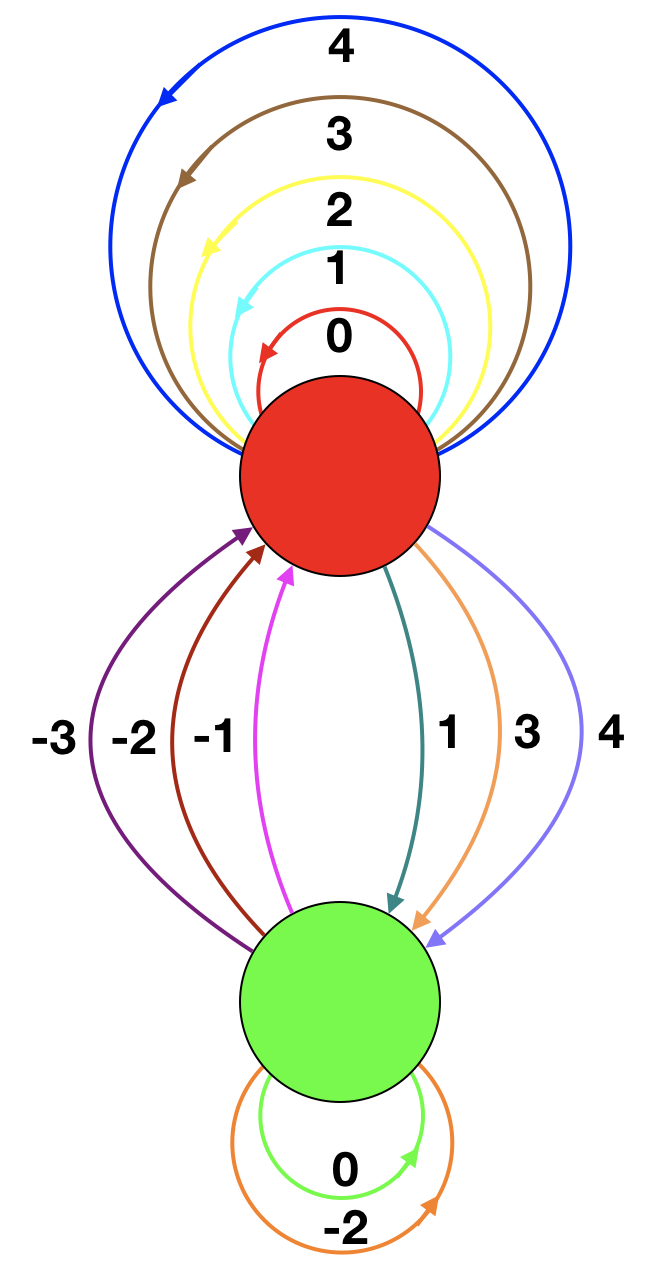
\includegraphics[width=1.0\textwidth]{PVAWMarkov2Steps}\\(d)
            \end{center}\end{minipage}
\end{center}
  \caption{\label{fig:PVAdlerWeiss2Steps}
(a)
An \AW\ one step forward in time partition of the unit torus for the
$s=3$ \PV\ cat map \reffig{fig:PVAdlerWeissB}\,(c).
(b)
Mapped two steps forward in time, the rectangles are stretched along the
unstable direction and shrunk along the stable direction. Sub-rectangles
$\pS_j$ that have to be translated back into the partition are indicated by
color and labeled by their lattice translation
$\Ssym{j}$.
(c)
The sub-rectangles $\pS_j$ translated back into the unit square yield a
two steps forward in time
generating partition (a subpartition of rectangles in (a)), with
(d)
the finite grammar given by the {\markGraph} for this partition. The nodes
refer to the rectangles $A$ and $B$, and the 13 links correspond to the 13
sub-rectangles induced by two step forward-in-time dynamics.
}
\end{figure}
%%%%%%%%%%%%%%%%%%%%%%%%%%%%%%%%%%%%%%%%%%%%%%%%%%%%%%%%%%%%

%%%%%%%%%%%%%%%%%%%%%%%%%%%%%%%%%%%%%%%%%%%%%%%%%%%%%%%%%%%%%
\begin{figure}
  \centering
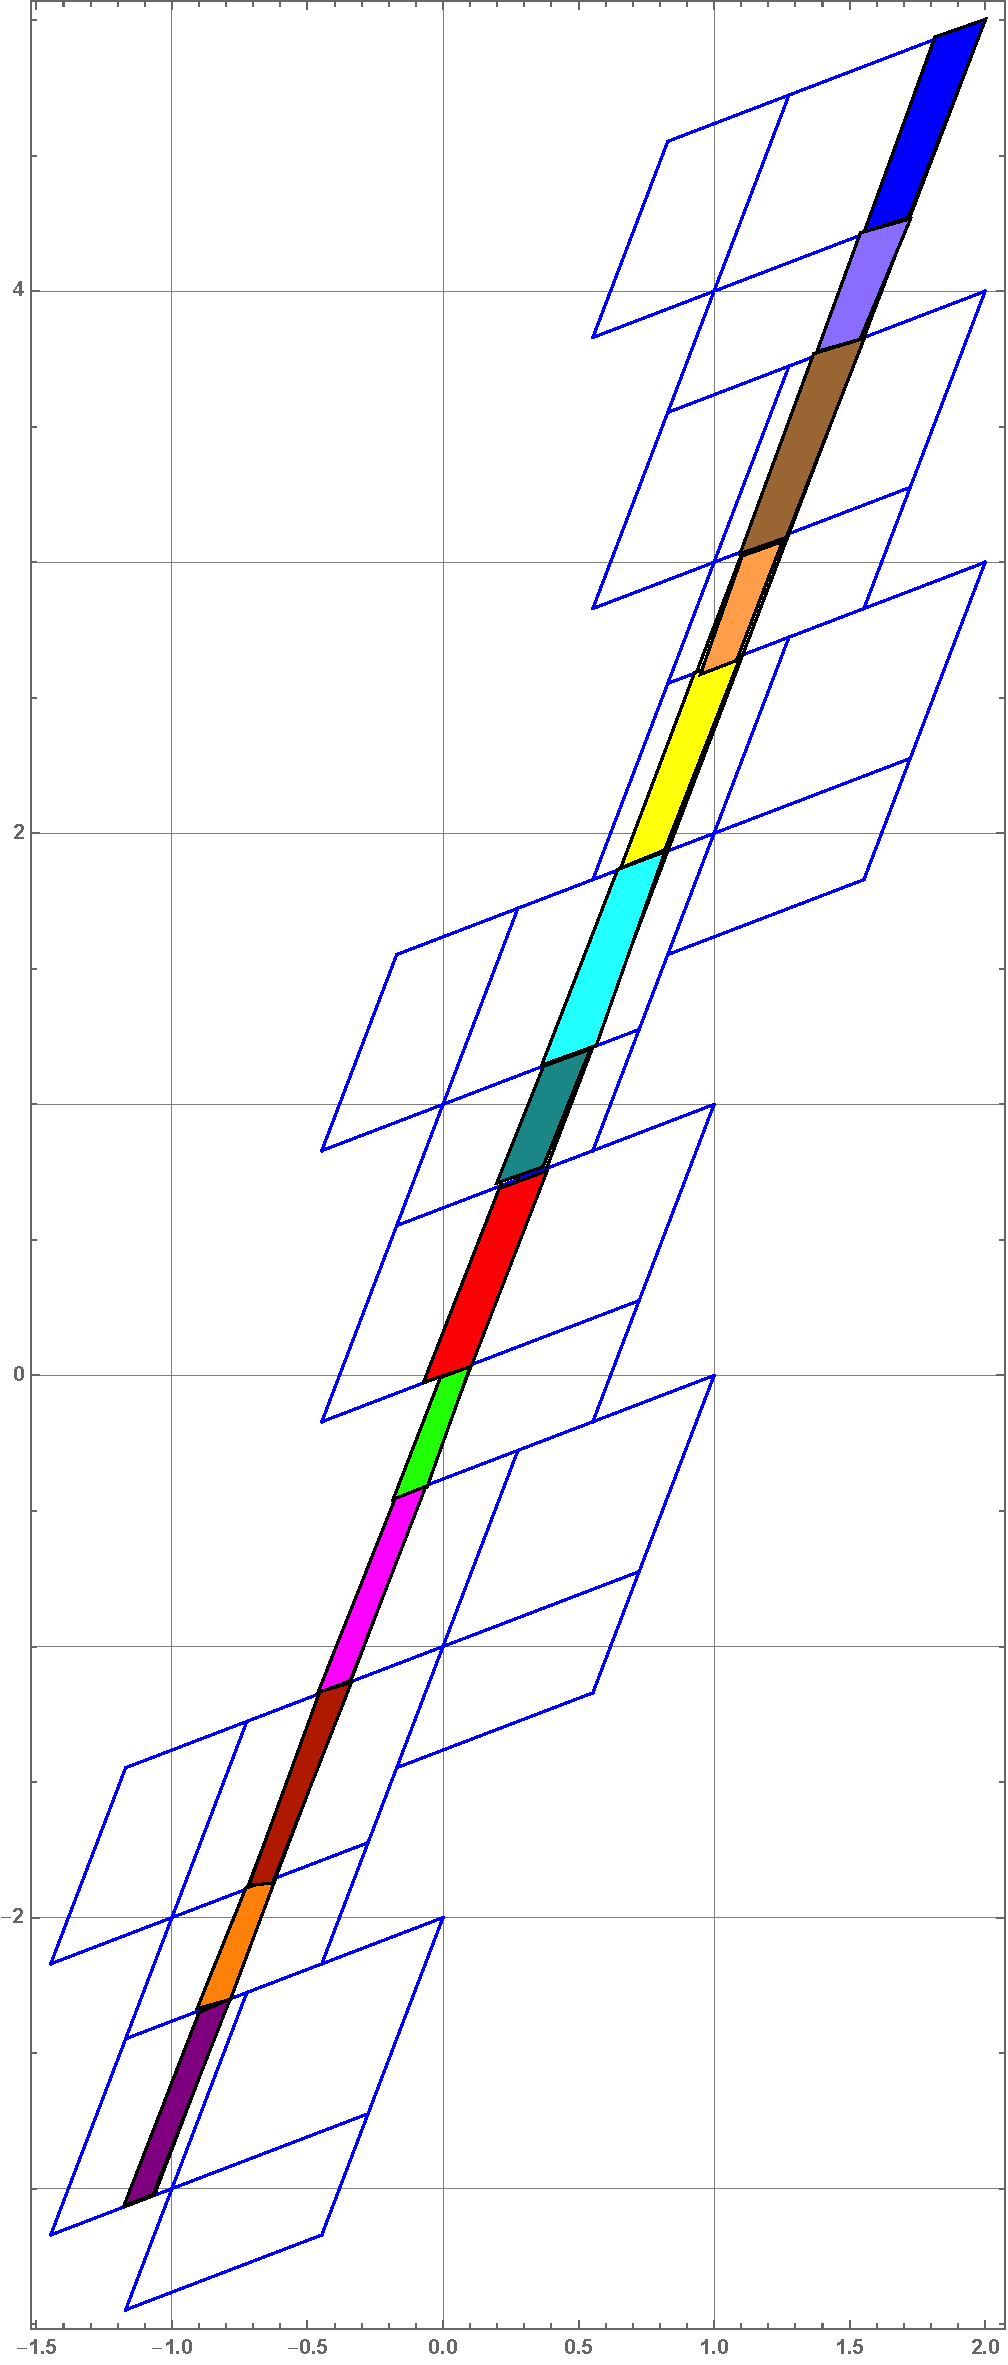
\includegraphics[width=0.40\textwidth]{PVAdlerWeiss2Steps-d}
  \caption{\label{fig:PVAdlerWeiss2StepsD}
This figure is used to track where each sub-rectangles in
\reffig{fig:PVAdlerWeiss2Steps} goes. Note that two step forward-in-time
requires both vertical and horizontal shifts, unlike the one step
forward-in-time \PV\ cat map \refeq{eq:StateSpCatMap}.
}
\end{figure}
%%%%%%%%%%%%%%%%%%%%%%%%%%%%%%%%%%%%%%%%%%%%%%%%%%%%%%%%%%%%%%%

\refFig{fig:PVAdlerWeiss2Steps} is a very nice illustration
of a generating partition subrectangles being further subdivided.
} % end \solution{exer:n=2GenPart}
%%%%%%%%%%%%%%%%%%%%%%%%%%%%%%%%%%%%%%%%%%%%%%%%%%%%%%%%%%%%%%%%%%%



\ChapterEnd % formatted for ChaosBook.org
